%\documentclass[showinstructions,faculty=fbiw,department=bsy,doctoralschool=ads]{adsphd}
\documentclass[tothejury,faculty=fbiw,department=bsy,doctoralschool=ads]{adsphd}

%\documentclass[showinstructions,showlabels,coverfontpercent=100,faculty=firw,department=cws,phddegree=cws]{adsphd}
%\documentclass[croppedpdf,showinstructions,faculty=firw,department=cws,phddegree=cws]{adsphd}
%\documentclass[online,faculty=firw,department=cws,phddegree=cws]{adsphd}
%\documentclass[print,bleed,cropmarks,faculty=firw,department=cws,phddegree=cws]{adsphd} % include bleed for the print service
%\documentclass[print,faculty=firw,department=cws,phddegree=cws]{adsphd}
%\documentclass[final,faculty=firw,department=cws,phddegree=cws]{adsphd}
%\documentclass[showinstructions,faculty=firw,department=cws,phddegree=cws,epub]{adsphd}

% !!!!!!!!!!!!!!!!!!!!!!!!!!!!!!!!!!!!!!!!!!!!!!!!!!!!!!!!!!!!!!!!!!!
% !!                                                               !!
% !!  WARNING: do not remove the following lines between           !!
% !!  "%%% COVER: Settings %%%" and "%%% COVER: End settings %%%"  !!
% !!                                                               !!
% !!!!!!!!!!!!!!!!!!!!!!!!!!!!!!!!!!!!!!!!!!!!!!!!!!!!!!!!!!!!!!!!!!!

%%% COVER: Settings %%%
\title{Optimal Experimental Design for Dynamic Systems}
\subtitle{Towards more efficient experimentation in post-harvest storage of fruit and vegetables}

\author{Arno}{Strouwen}

\supervisor{Prof.~dr.~Peter Goos}{}
\supervisor{Prof.~dr.~ir.~Bart Nicolaï}{}
\president{Prof.~dr.~ir.~René~De~Mot}{}
\jurymember{Prof.~dr.~ir.~Kristel~Bernaerts}{}
\jurymember{Prof.~dr.~ir.~Wouter~Saeys}{}
\externaljurymember{Prof.~dr.~Julio~Banga}{Instituto de Investigacións Mariñas-\\Consejo Superior de Investigaciones Científicas}
\externaljurymember{Dr.~ir.~Philippe~Nimmegeers}{Universiteit Antwerpen}

% Your research group within the department
% e.g. iMinds-DistriNet, Scientific Computing Group, ...
\researchgroup{MeBioS}
\website{} % Leave empty to hide
\email{arno.strouwen@kuleuven.be} % Leave empty to hide

\address{Kasteelpark Arenberg 30}
% \addresscity{B-3001 Leuven} % This is the default value. Note
                              % that 'B-3001 Heverlee' is _incorrect_!!
                              % /[https://www.kuleuven.be/communicatie/marketing/intranet/huisstijl/taalgebruik.html]
\date{August 2021}
\copyyear{2021}
%\udc{XXX.XX}            % UDC, deposit number and ISBN are no longer necessary.
%\depot{XXXX/XXXX/XX}    % Leave out the initial D/ (it is added
                         % automatically)
%\isbn{XXX-XX-XXXX-XXX-X}


% Set spine width:
\setlength{\adsphdspinewidth}{9mm}

%% Set bleeds
%\setlength{\defaultlbleed}{7mm}
%\setlength{\defaultrbleed}{7mm}

% Set custom cover page
% \setcustomcoverpage{mycoverpage.tex} % mycoverpage.tex is the default

%%% COVER: End settings %%%

% BibLaTeX
\usepackage[utf8]{inputenc}
%\usepackage{csquotes}
\usepackage[
  hyperref=auto,
  mincrossrefs=999,
  backend=biber,
  style=authoryear]{biblatex}
\addbibresource{ref/1.bib}
\addbibresource{ref/2.bib}
\addbibresource{ref/3.bib}
\addbibresource{ref/conclusion.bib}

% Fonts
\usepackage{textcomp} % nice greek alphabet
\usepackage{pifont}   % Dingbats
\usepackage{booktabs}
\usepackage{amssymb,amsthm}
\usepackage{amsmath}


%%%%%%%%%%%%%%%%%%%%%%%%%%%%%%%%%%%%%%%%%%%%%%%%%%%%%%%%%%%%%%%%%%%%%%
% MY PACKAGES

\providecommand{\e}[1]{\ensuremath{\times 10^{#1}}} % scientific notation power
\DeclareMathOperator{\dd}{\mathrm{d}}
\DeclareMathOperator{\Tr}{\mathrm{Tr}}
\DeclareMathOperator{\Covar}{\mathrm{Covar}}
\DeclareMathOperator{\Var}{\mathrm{Var}}
\DeclareMathOperator{\E}{\mathrm{E}}
\DeclareMathOperator*{\argmax}{arg\,max}
\DeclareMathOperator*{\argmin}{arg\,min}
\newcommand{\Coxy}{[\text{O}_2]}
\newcommand{\oxy}{\text{O}_2}
\newcommand{\Ccoxy}{[\text{CO}_2]}
\newcommand{\coxy}{\text{CO}_2}

% math 
\usepackage{esdiff}
\usepackage{nicefrac}
\usepackage{bm} % bold math

% figure tables algo ...
\usepackage{enumitem}
\usepackage{numprint}
\usepackage[ruled,lined]{algorithm2e}
\usepackage{subcaption}
\usepackage{float}

\usepackage{tikz}
\usetikzlibrary{shapes,arrows,positioning,external}
\usetikzlibrary{calc,patterns,decorations.pathmorphing,decorations.markings}

% font stuff



\begin{document}
\makefrontcoverXII
\maketitle
\frontmatter % to get \pagenumbering{roman}
\include{chapters/preface}
\chapter*{Abstract}
Living systems are rife with variability. Well-chosen experimental designs are necessary to deal with this variability when modeling such systems. Models for living systems often rely on knowledge of physical, chemical and biological laws, such as mass balances, transport phenomena and reaction kinetics, and are often described by a system of non-linear differential equations. So, the structure of a model can often be determined from first principles. However, the model will generally also rely on parameters whose numerical values cannot be determined from physical laws. These parameters must then be inferred from experimental data before the model can be put to use. A well-chosen experiment can greatly improve the estimation of the model parameters. But there exist several challenges for constructing such informative experiments for dynamic systems. One challenges is the dependence of the optimal experiment on the true model parameters, making it difficult to perform robust experiments that work well regardless of the specific model parameter values. Another challenge is the correlation of the observations due to the presence of process noise. The central research topic of this thesis revolves around solving these challenges by developing robust experimental design methodology for noisy dynamic systems. My novel methodology is developed to improve postharvest applications, and is mainly applied to the estimation of respiration and fermentation parameters of pear fruit. 
\\
\\
After an introduction in the first chapter, the second chapter of this PhD thesis deals with the estimation of respiration parameters of pear fruit inside a jar, modeled by Michaelis-Menten kinetics. Air flowing into the jar has to be controlled so that the parameters of the Michaelis-Menten model can be estimated as precisely as possible. The quality of this parameter estimation, and thus of the experimental design, is quantified using the determinant of the Fisher information matrix, which is inversely related to the area of the confidence ellipse of the two Michaelis-Menten model parameters. The air flowing into the jar must thus be optimized so that the determinant of the Fisher information matrix is as large as possible. One major challenge here is the dependence of this Fisher information matrix on the true, but unknown, parameters of the system. The most commonly used method in the literature to deal with this issue is locally optimal design, where a single initial guess is used for the true parameter. One main conclusion from my work is that this optimal experimental design technique outperforms several commonly used heuristic experimental techniques.
\\
\\
The third chapter builds on the first but also takes fermentation of the pear fruit into account. The locally optimal design method only takes into account a single initial guess, and may not perform well if this guess deviates substantially from the true parameter values. Instead of a single initial guess, an entire distribution could be used to quantify the prior knowledge and uncertainty on the unknown parameters. Because of the use of a prior distribution, this method is called Bayesian experimental design. Most current techniques in the literature only allow for parametric prior distributions, such as normal distributions. The prior information about respiration and fermentation, coming from a previously gathered dataset, could not be summarized by any parametric distribution. For this reason, I developed a novel experimental design technique based on a Markov-chain Monte-Carlo (MCMC) analysis of this previously gathered data. This method is thus able to approximate arbitrary distributions. I found that this flexible experimental design technique is more robust than the commonly used locally optimal design method.
\\
\\
The fourth chapter focuses on robust and adaptive experimental design techniques for dynamic systems with process noise. Current experimental design techniques for dynamic systems generally only incorporate measurement noise, but biological systems also often involve process noise. Calculating the Fisher information matrix for such systems requires estimating the uncertain dynamic states, using Bayesian filtering techniques. For linear dynamical systems, the optimal filter is the Kalman filter. But deriving the Fisher information matrix for dynamic systems under process noise and then applying the methodology from the previous chapters is not sufficient to construct informative experiments. This is due to the difficulty in precisely predicting such systems far into the future, which causes those future measurements to contribute little to the Fisher information matrix. Adaptive experimental designs are able to deal with this issue. Adaptive designs use the already gathered data to re-optimize and thus adapt the remainder of the experiment. The already gathered measurements can help by reducing the uncertainty on the model parameters, which the optimal design depends upon. Adaptivity is thus always a good design strategy, even when no process noise is present. But for systems with process noise, adaptivity is even more important, since the already gathered measurements help increase the prediction accuracy of future measurements, thus increasing the informativity of these measurements. I found that taking into account process noise in the experimental design greatly improves the quality of the experiment.
\chapter*{Beknopte Samenvatting}
Levende systemen worden gekenmerkt door een grote maat aan variabiliteit. Goed gekozen experimentele ontwerpen zijn noodzakelijk om goed om te gaan met deze variabiliteit. Modellen van levende systemen steunen vaak op kennis van fysieke, chemische of biologische wetten, zoals massabalansen, transportverschijnselen en reactiekinetiek, en worden vaak beschreven door een systeem van niet-lineaire differentiaalvergelijkingen. Dus, de structuur van het model kan vaak bepaald worden door eerste principes. Echter, het model zal in het algemeen ook afhangen van parameters waarvan de numerieke waarden niet kunnen vastgesteld worden door fysieke wetten. Deze parameters moeten dan afgeleid worden uit experimentele data voordat het model toegepast kan worden. Een goed gekozen experiment kan de schatting van deze parameters sterk verbeteren. Er bestaan echter verschillende uitdagingen bij het opstellen van zo een informatief experiment voor dynamische systemen. Een eerste uitdaging is de afhankelijkheid van het optimale experiment van de waarden van de modelparameters, wat het moeilijk maakt om robuuste experimenten op te zetten die goed werken voor om het even welke modelparameterwaarden. Een andere uitdaging is de correlatie tussen de observaties door de aanwezigheid van procesruis. Het centrale onderzoeksthema van deze thesis draait rond het aanpakken van deze uitdagingen door het ontwerpen van een robuuste methodologie voor experimenteel ontwerp voor dynamische systemen met ruis. Mijn nieuwe methodologie is ontworpen om naoogsttoepassingen {\color{red}en andere toepassingen in het domein van de bio-ingenieurswetenschappen} te verbeteren, en is voornamelijk gericht op de schatting van respiratie- en fermentatieparameters van peren. {\color{red}Experimenten die toelaten om de modelparameters van massa-veer-demper systemen en compartiment systemen precies te schatten worden evenwel ook opgesteld}.
\\
\\
{\color{red}Na een korte inleiding over experimenteel ontwerp voor dynamische systemen en de toepassingsgebieden ervan}, behandelt deze doctoraatsthesis het schatten van respiratieparameters van peer in een pot, gemodelleerd met behulp van Michaelis-Menten kinetiek. Lucht die de pot instroomt kan aangestuurd worden zodat de parameters van het Michaelis-Menten model zo precies mogelijk kunnen geschat worden. De kwaliteit van deze parameterschatting, en dus ook het experimenteel ontwerp, wordt gekwantificeerd door middel van de determinant van de Fisher informatiematrix, die omgekeerd gerelateerd is aan de betrouwbaarheidsellips van de twee Michaelis-Menten modelparameters. Lucht die de pot instroomt moet geoptimaliseerd worden zodat de determinant van de Fisher informatiematrix zo groot mogelijk is. Een grote uitdaging is het feit dat deze Fisher informatiematrix afhangt van de (onbekende) modelparameters. De meest gebruikte techniek in de literatuur voor het omgaan met deze kwestie is lokaal optimaal ontwerp, waarbij een enkele initiële gok wordt gebruikt voor de echte parameters. De belangrijkste conclusie van mijn werk is dat dit optimaal experimenteel ontwerp verscheidene vaak gebruikte heuristische methodes van experimenteel ontwerp overtreft.
\\
\\
{\color{red}Vervolgens brengt de thesis ook de fermentatie van peerfruit in rekening}. Het lokaal optimaal ontwerp houdt alleen rekening met een enkele initiële gok, en presteert doorgaans niet goed als deze gok substantieel afwijkt van de echte parameterwaarden. In de plaats van een enkele initiële gok kan een ganse kansverdeling gebruikt worden om de a priori kennis en onzekerheid omtrent de modelparameters te kwantificeren. Omwille van het gebruik van een a priori verdeling wordt deze methode Bayesiaans experimenteel ontwerp genoemd. De meeste huidige technieken in de literatuur staan enkel parametrische a priori verdelingen toe. De a priori informatie over respiratie en fermentatie, waarover ik beschikte, kon niet samengevat worden door een parametrische kansverdeling. Om deze reden ontwierp ik een nieuwe techniek gebaseerd op een Markov-chain Monte-Carlo analyse van deze voorheen verzamelde data. Deze methode kan arbitraire kansverdelingen benaderen. Ik ontdekte dat deze flexibele techniek robuuster is dan de vaak gebruikte techniek van lokaal optimaal ontwerp, {\color{red}alsook andere robuuste methodes}.
\\
\\
{\color{red}Het laatste deel van de thesis richt} zich op robuuste en adaptieve technieken voor experimenteel ontwerp voor dynamische systemen met procesruis. De huidige technieken voor dynamische systemen kunnen enkel omgaan met meetruis, maar procesruis komt ook vaak voor in biologische systemen. Het berekenen van de Fisher informatiematrix voor dergelijke systemen vereist het schatten van de onzekere dynamische toestanden met behulp van Bayesiaanse filtertechnieken. Voor lineaire dynamische systemen is de optimale filter de Kalman filter. Echter, het afleiden van de Fisher informatiematrix voor dynamische systemen onder procesruis en vervolgens de methodologie uit de voorgaande hoofdstukken toepassen volstaan niet om informatieve experimenten op te stellen. Dit is te wijten aan de moeilijkheid om dergelijke systemen ver in de toekomst nauwkeurig te voorspellen, waardoor metingen ver in de toekomst weinig bijdragen aan de Fisher informatiematrix. Adaptieve experimentele ontwerpen zijn in staat om dit probleem te remediëren. Adaptieve ontwerpen gebruiken de reeds verzamelde gegevens om de rest van het experiment opnieuw te optimaliseren en dus aan te passen aan de vrijgekomen informatie. De reeds verzamelde metingen helpen de onzekerheid te verminderen omtrent de modelparameters, waarvan het optimale ontwerp afhankelijk is. Adaptiviteit is dus altijd een goede ontwerpstrategie, ook als er geen procesruis aanwezig is. Maar voor systemen met procesruis is adaptiviteit nog belangrijker dan voor systemen zonder procesruis, omdat de reeds verzamelde metingen de nauwkeurigheid van de voorspellingen van toekomstige metingen helpen te vergroten, waardoor de informativiteit van deze metingen toeneemt. In mijn derde hoofdstuk demonstreerde ik dat het beschouwen van procesruis in het experimentele ontwerp de kwaliteit van het experiment aanzienlijk verbetert.

\chapter*{List of Abbreviations}
\begin{itemize}[labelwidth={0em},font=\bfseries,align=right]
\item [BLUE] best linear unbiased estimator
\item [DCA] dynamic controlled atmosphere
\item [FIM] Fisher information matrix. When used without further specification, refers to the expected Fisher information matrix, as opposed to observed Fisher information matrix.
\item [KL-div] Kullback-Leibler divergence
\item [MAP] modified atmosphere packaging
\item [MCMC] Markov-chain Monte-Carlo
\item [SSE] sum of squared error
\end{itemize}


\tableofcontents
\listoffigures
\listoftables
\mainmatter % to get \pagenumbering{arabic}
\chapter{Introduction}
\section{Motivation}
{\color{red}Experimentation is required in almost all areas of bio-science engineering. A well chosen experimental design can tremendously reduce this required experimental effort. One area of bio-science engineering that requires a lot of experimentation is the postharvest storage of fruit and vegetables.}
\\
\\
Fresh fruit and vegetables are perishable and need to be stored at appropriate conditions after their harvest. The temperature is typically set as low as possible to reduce respiration, but above the freezing point of the product. Below this point, massive cell damage occurs and the product no longer can be considered as fresh. A further reduction of the respiration rate is possible by reducing the $\oxy$ partial pressure of the storage atmosphere and increasing its $\coxy$
partial pressure. 

The optimal storage conditions (temperature, $\oxy$ and $\coxy$ partial pressures) of fruit and vegetables depend on the species, cultivar, ripeness stage and many other factors and must be experimentally determined. Traditionally, this has been achieved by storing the product at many combinations of temperature, $\oxy$ partial pressure and $\coxy$ partial pressure, and monitoring the change in quality attributes during the storage period. This can be as much as one year for apple and pear fruit.
\\
\\
As an alternative, a mathematical model based approach could be used to optimize storage protocols. This approach relies on comprehensive mathematical models that describe the behavior of the product as a dynamical system with inputs (temperature, $\oxy$ partial pressure and $\coxy$  partial pressure) and outputs (respiration and fermentation rate, quality attributes), based on physical, chemical and biological laws. {\color{red}These mathematical models rely on parameters whose numerical values cannot be determined from first laws, and must be experimentally determined. The experimental effort then shifts from parameter estimation for black box response surface models to parameter estimation for mechanistically based differential equation models. We then no longer have to independently test the fruit and vegetables at different storage conditions via a factorial design. Instead, one single experiment involving time varying $\oxy$ and $\coxy$ partial pressures would allow us to estimate the respiration and fermentation parameters of the differential equation models. The latter can subsequently be used to simulate the behavior of the fruit in arbitrary storage conditions, and the optimization of the storage process can then be done in silico \parencite{tri}. This shift towards mathematical models also allows us to use model based experimental design methods \parencite{franceschini}. The challenge is to construct optimal time-varying $\oxy$ and $\coxy$ partial pressures such that the respiration and fermentation parameters can be precisely estimated in a single experiment.}
\\
\\
{\color{red}Besides improving postharvest experimentation, the methods we derive in this thesis are much more broadly applicable and can be used to design experiments for the precise estimation of model parameters in many differential equation models in other fields of bio-science engineering and engineering.}
\section{Goals}
The general goal of this thesis is to develop the statistical methodology required to create dynamic inputs that lead to precise parameter estimation for non-linear differential equation models. In Chapters \ref{paper1} and \ref{paper2}, we apply this to the estimation of respiration and fermentation parameters of pear fruit. {\color{red}In Chapter \ref{paper3}, experiments to estimate the model parameters of spring-mass-damper systems as well as compartment systems are constructed.} In doing so, several challenges  must be overcome:
\begin{itemize}
	\item \textbf{Challenge 1}. Constructing optimal experiments for non-linear dynamic systems is a circular problem, as the best experiment to learn about the model parameters depends on the specific values of those parameters. Some form of prior information about the model parameters is required to solve this issue.
	\item \textbf{Challenge 2}. If the prior information required in \textbf{Challenge 1} were perfect, then no further experiments would be needed. Generally, however, there is substantial uncertainty concerning the prior information. Therefore, a robust experimental design is desired that performs well over a range of possible parameter values. {\color{red}Current robust experimental design methods are only capable of achieving robustness when this prior information is summarized well with a parametric distribution. However, not all prior information can easily be summarized in such a way. To overcome this challenge, a non-parametric method should be developed.}
	\item \textbf{Challenge 3}. Current experimental design methodology ignores process noise. Often, all errors are attributed to measurement noise. {\color{red}In the presence of process noise, the challenge lies in generalizing the definition of the Fisher information matrix to deal with observations that are correlated in time.}
	\item \textbf{Challenge 4}. Adapting the experimental design using information from measurements as they are being gathered is another way to deal with the dependence of the optimal experiment on the true parameters. {\color{red}Current experimental design methodology, in the context of differential equation models in combination with process noise, is not suitable for online computation. This is because of} the growing complexity of the optimization problem over time, particularly when also dealing with process noise. {\color{red}An alternative experimental design method with constant memory and time complexity therefore has to be developed.}
\end{itemize}
\section{Chapter by Chapter Overview}
\begin{itemize}
	\item \textbf{Chapter \ref{paper1}} uses the traditional locally optimal experimental design method to optimize oxygen input profiles, which lead to a precise estimation of respiration parameters {\color{red}of pear fruit}. This method deals with the dependence of these input profiles on the true respiration parameters, described in \textbf{Challenge 1}, by requiring an initial guess for these parameters. This initial guess is provided by a parameter estimate from the literature.
	\item \textbf{Chapter \ref{paper2}} addresses \textbf{Challenge 2} by developing a robust experimental design method involving a quantification of the uncertainty about the model parameters by applying a Markov-chain Monte-Carlo technique to a prior data-set. This robust experimental design method is then used to jointly optimize both  $\oxy$ and $\coxy$ input profiles to precisely estimate both respiration and fermentation parameters of pear fruit.
	\item \textbf{Chapter \ref{paper3}} uses the Kalman filter to deal with \textbf{Challenge 3} of experimental design under process noise. This filter is used to track an estimate of the hidden states over time. This estimate is required to calculate the likelihood of the model parameters, which in turn is required to calculate the Fisher information matrix for these more complicated dynamic systems with process noise. The state estimate is also required for \textbf{Challenge 4} concerning adaptive designs, as we need information about the true state of the system when redesigning the remainder of the experiment. The issue of growing complexity of the optimization problem over time is dealt with by using a combination of the observed and expected Fisher information matrix.
	\item \textbf{Chapter \ref{conclusion}} {\color{red}presents} an overarching conclusion of the work done in my thesis. This chapter also gives an overview of alternative or related experimental design strategies for dynamic systems, as well as an overview of numerical methods that might improve the speed or precision with which an optimized experiment can be constructed. I also discuss future research prospects that might grow out of the techniques described in this thesis.
\end{itemize}
\cleardoublepage
\chapter{Optimizing Oxygen Input Profiles for Efficient Estimation of Michaelis-Menten Respiration Models}
\label{paper1}
This chapter has been published in Food and Bioprocess Technology.\footnote{\textbf{Strouwen, A.}, Nicolaï, B.M., Goos, P. (2019). Optimizing Oxygen Input Profiles for Efficient Estimation of Michaelis-Menten Respiration Models. Food and Bioprocess Technology, 12 (5), 769-780. }
\\
\\
{\color{red}Source code available upon request.}
\section*{Abstract}
Models based on mass balances and Michaelis-Menten respiration kinetics are increasingly used to determine optimal storage conditions of fresh fruits and vegetables. The model parameters are usually estimated from respiration experiments at different, but fixed, gas conditions according to a response surface design. This is a tedious procedure that requires a gas mixing facility or a series of gas cylinders with appropriate composition. In this chapter, we consider a simpler approach, in which the respiration kinetics of pear fruit are modeled using a single experiment with a time varying $\text{O}_2$ input profile. To optimize the information content produced by the $\text{O}_2$ profile, we apply optimal dynamic experimental design principles and present a modified coordinate-exchange algorithm to achieve this goal. Finally, we demonstrate the added value of our approach by comparing the optimal $\text{O}_2$ input profiles to several intuitive benchmark experiments.
\section{Introduction}
Fresh fruit needs to be stored at appropriate temperature as well as $\text{O}_2$ and $\text{CO}_2$ conditions, after its harvest. The ideal storage conditions depend on the species, cultivar, ripeness stage and many other factors, and must be experimentally determined. Traditionally, this is achieved by independently storing fruit at many different combinations of temperature as well as $\text{O}_2$ and $\text{CO}_2$ partial pressures, and by monitoring the change of quality attributes during, the sometimes year long, storage period \parencite{fidler}. The optimal storage conditions are then inferred from response surface modeling. This method is black box in nature and labor intensive, due to the large number of time-consuming experimental combinations that have to be tested \parencite{saltveit}.
\\
\\
Many modern {\color{red}storage} applications, such as modified atmosphere packaging (MAP) \parencite{MAP1,MAP2} and dynamic controlled atmosphere (DCA) \parencite{bessemans}, rely on knowledge of mass balances, transport phenomena and reaction kinetics, and use comprehensive mathematical models that describe the behavior of the product as a dynamical system with inputs (temperature, $\text{O}_2$ and $\text{CO}_2$ partial pressures) and outputs (respiration and fermentation rate, quality attributes). The respiration kinetics are a key feature of such dynamic models, and are generally described by a non-linear model of the Michaelis-Menten type \parencite{maarten1}. The standard Michaelis-Menten model contains two parameters: the maximum respiration rate and the affinity or Michaelis-Menten constant \parencite{peppelenbos}.
\\
\\
Michaelis-Menten kinetics are generally used to describe the kinetics of a simple enzymatic pathway in which, first, a substrate-enzyme complex is formed in a reversible way. In a second rate limiting step, the complex dissociates into the reaction product and the enzyme \parencite{michaelismenten}. Although respiration, and specifically $\text{O}_2$ consumption, is a far more complex pathway, that contains both linear and circular routes and a multitude of intermediate compounds \parencite{berg}, it can be described surprisingly well by Michaelis-Menten like kinetics at various spatial scales, from the fruit tissue level to the intact fruit level \parencite{tri}. The maximum respiration rate and the Michaelis-Menten constant should thus be considered as apparent parameters, that summarize the behavior of the more complex pathway underneath. These parameters are typically estimated from respiration experiments at various combinations of temperature as well as $\text{O}_2$ and $\text{CO}_2$ partial pressure, which are then kept constant throughout the experiment. Appropriate experimental design techniques are then applied to reduce the number of experimental runs. Typically, response surface designs, such as central composite designs, are used to define the combinations to be tested, and response surface models are fitted to the resulting data. However, even then, the experimental effort remains considerable {\parencite{fidler,saltveit}}.
\\
\\
Alternatively, dynamic experiments can be conceived in which the experimental factors may vary over time in such a way that they maximize the information content of the experimental data set. The shift from traditional response surface modeling towards dynamic models for estimating  respiration kinetics entails unique challenges for designing experiments. As we explain below, this is due to the fact that the former modeling approach is based on linear algebraic equations and parameter estimation, while the latter requires differential equations and non-linear parameter estimation. 
\\
\\
The optimal design of dynamic experiments is an unexplored research topic within postharvest research and fruit storage. It has, however, received a limited amount of attention in other biological fields. One example is the construction of an optimal temperature profile to aid the estimation of several kinetic growth parameters in predictive microbiology \parencite{bernaerts1,bernaerts2,balsa1}. Another example can be found in food engineering, where temperature profiles have to be optimized to better determine thermo-physical properties of food products \parencite{nahor1,nahor2}. However, applications are not limited to temperature profiles. For instance, during the identification of biochemical networks, the input profile of several (bio-)chemical substances has to be controlled \parencite{balsa2}. This is similar to our own problem, where an $\text{O}_2$ input profile has to be optimized.
\\
\\
In this chapter, we show how to design dynamic experiments to efficiently estimate the two Michaelis-Menten respiration parameters of the specific oxygen consumption rate of pear fruit. First, in Section \ref{Model}, we present a model for pear fruit respiring inside a jar, with $\text{O}_2$ as the sole time varying input. In Section \ref{Information}, we introduce the main concepts of optimal dynamic experimental design and we subsequently apply them to our model to derive expressions for quantifying the information content of an experiment. In Section \ref{Optimization}, We propose two methods to optimize the information content of the experiment, based on the coordinate-exchange algorithm. In Section \ref{Results}, we construct three optimal designs for different admissible input profiles. The first proof of concept design in Section \ref{Experiment1} is constructed assuming that the $\text{O}_2$ input level can only be modified every $2 \text{ h}$, and is either in an on or an off state. In Section \ref{Refinement}, two optimal designs are constructed  by relaxing the restrictions on the input profile in two different ways. First, by allowing the input to be modified every $10 \text{ min}$. And secondly, by allowing $11$ possible input levels. Our decisions on how to quantify information, and on how to parametrize the input profile are discussed in Section \ref{Discussion}, as well as some alternatives. We also discuss further research options in this section.
\section{Methods}
The methods section is divided into three parts. First, we propose a respiration model for pear fruit, in an experimental unit: the jar. Next, we discuss the main concepts of optimal dynamic experimental design and apply them to our model. Finally, we adapt the coordinate-exchange algorithm to work better for the dynamic experiments considered in this chapter.
\subsection{Dynamic Model for Respiration}
\label{Model}
The respiration of pear fruit inside a jar was modeled using the following mass balance,
\begin{equation}
\label{systemP1}
V_\text{j}\diff{C_\text{m}}{t}(t) = Q(t)(C_{\text{in}} - C_\text{m}(t)) - m_\text{p}r(t),
\end{equation}
where $C_\text{m}(t)$ is the modeled $\text{O}_2$ concentration in the jar $[\text{mol m}^{-3}] $, at time $t$ $[\text{s}]$. The left-hand side of the equation shows the change of mass inside the jar, with a volume $V_\text{j}$ of $5\text{ dm}^3$. The right-hand side consists of two terms, the first of which describes the air flowing in and out of the jar. The flow rate $Q(t)$ $[\text{m}^3\text{ s}^{-1}]$ is the controllable input to the system. More specifically, we assumed that air is blown into the jar with concentration $C_{\text{in}}$ equal to that of regular air (21 volume \%), and that, air flows out of the system at the same rate $Q(t)$ and with the same $\text{O}_2$ concentration $C_\text{m}(t)$ as that inside the jar, due to the assumption of perfect mixing. The second term in the right-hand side models the consumption of $\text{O}_2$ inside the jar, which is proportional to the mass of the pears, $m_\text{p}$ $[\text{kg}]$. Throughout the chapter, we assumed that all measurements are performed on $4 \text{ kg}$ of pears. The reaction rate $r(t)$ $[\text{mol kg}^{-1}\text{s}^{-1}]$, at time $t$ is described by the Michaelis-Menten kinetics model,
\begin{equation}
r(t) = \frac{V_{\text{max}}C_\text{m}(t)}{K_\text{m} + C_\text{m}(t)},
\end{equation}
in which the maximal respiration rate $V_{\text{max}}$ $[\text{mol kg}^{-1}\text{s}^{-1}]$ and the Michaelis-Menten constant $K_\text{m}$ $[\text{mol m}^{-3}]$ are the two unknown parameters. In using this model, we ignored the effect of fermentation at low oxygen concentration. The jar was assumed to be filled with (regular) air at the start of every experiment. A representation of the model is given in Figure \ref{figJar}. Finally, we assumed that the measured concentration $C(t)$ only differs from the modeled concentration by an additive white noise term $\epsilon(t)$:
\begin{equation}
C(t) = C_\text{m}(t) + \epsilon(t).
\end{equation}
{\color{red}We also assume that the composition of the gas concentration in the jar is measured after sampling by means of a syringe through a septum in the lid of the jar.}
\begin{figure}
	\centering
	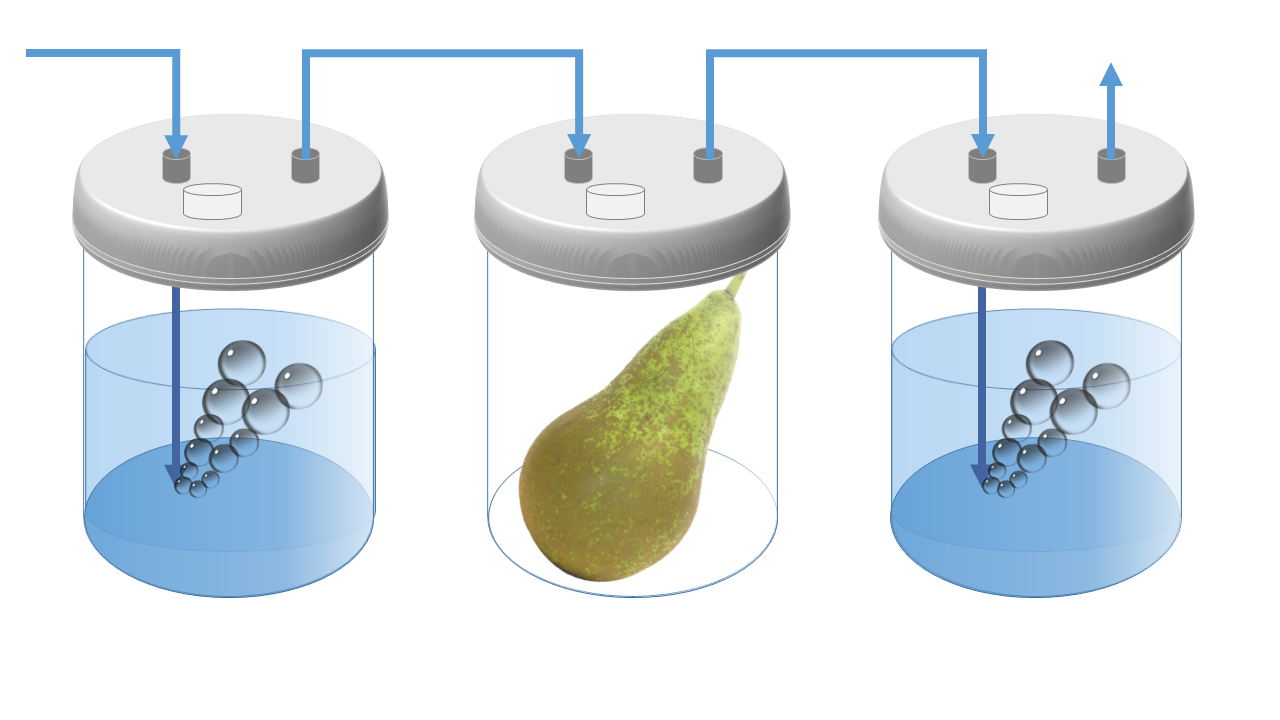
\includegraphics[width=0.8\textwidth]{figure/paper 1/pot.png}
	\caption{Graphical representation of the respiration jar measurement setup.}
	\label{figJar}
\end{figure}
\subsection{Optimal Experimental Design Methodology}
\label{Information}
Estimation of the parameter vector $\mathbf{p} = \begin{bmatrix}V_{\text{max}} & K_{\text{m}}\end{bmatrix}'$ was done by minimizing the squared error identification functional:
\begin{equation}
\mathbf{J} = \int_{0}^{t_\text{f}} (C(t) - C_\text{m}(\mathbf{p},Q(t),t))^2 \dd{t},
\label{J}
\end{equation}
where $t_\text{f}$ $[s]$ is the end time of the experiment. The functional $\mathbf{J}$ is often called the cost function.  This estimation problem was solved using the non-linear least squares algorithm, which required a starting value $\mathbf{p}^0$ for the parameters. Around that starting value, the model and $\mathbf{J}$ were linearized in the first iteration of the algorithm. When using that approach, the contours of $\mathbf{J}$ are ellipses, whose principal axes and surface area depend on the Fisher information matrix,
\begin{equation}
\mathbf{F} =  \int_{0}^{t_\text{f}}
\left(
\diff{C_\text{m}}{\mathbf{p}}
\right)'
\left(
\diff{C_\text{m}}{\mathbf{p}}
\right) \dd t,
\label{F}
\end{equation}
\parencite{fedorov}.The derivatives in this expression are generally referred to as parameter sensitivities:
\begin{equation}
\diff{C_\text{m}}{\mathbf{p}} =
\begin{bmatrix}
\dfrac{\partial C_\text{m}}{\partial V_{\text{max}}} & \dfrac{\partial C_\text{m}}{\partial K_{\text{m}}}
\end{bmatrix}.
\end{equation}
The larger the Fisher information matrix, the smaller the elliptic contours, and the steeper the cost functional $\mathbf{J}$ around its minimum, and thus the better the least squares identification problem is defined. The Fisher information matrix also has a second interpretation due to the fact that it is the inverse of the asymptotic variance covariance matrix of the best linear unbiased estimator (BLUE)  \parencite{munack1}. It summarizes the available information about the quality of the parameter estimates. The connection between the two interpretations of the Fisher information matrix is logical: the steeper the cost function, the better the least squares estimates fit the data compared to other parameter estimates. In that case, the quality of the estimates is large.
\\
\\
{\color{red}There exist more general definitions of the Fisher information matrix, which we use in subsequent chapters, in Sections \ref{secFIM2} and \ref{secFIM3}. The other definitions would lead to the same optimal respiration experiments presented in this chapter. However, the converse does not hold, the definition of the FIM in this chapter leads to different results in the other chapters.}
\\
\\
By modifying the input profile $Q(t)$, the magnitude of the Fisher information matrix, the steepness of the cost function and the surface areas of its contours can be optimized. To measure how large the Fisher information matrix is, different scalar functions of the Fisher information matrix have been proposed in the literature. These functions can be used to compare and score different experimental designs \parencite{atkinson1}. In this chapter, we used the determinant of the Fisher information matrix, $|\mathbf{F}|$, to compare different input profiles, which is referred to as the D-criterion. This criterion is inversely related to the area of the confidence ellipses of the parameter estimates, which should be minimal in an optimal experiment. Therefore, the optimized experimental design should maximize the determinant $|\mathbf{F}|$ over all admissible $\text{O}_2$ input profiles $Q(t)$:
\begin{equation}
\underset{\text{admissible Q(t)}}{\text{argmax}}|\mathbf{F}|.
\end{equation}
The parameter sensitivities $\dd C_\text{m}/\dd \mathbf{p}$ cannot be calculated analytically but have to be appended to the system of differential equations in equation (\ref{systemP1}), so they can be solved numerically. This is different from non-dynamical experiments, where analytical expressions exist for the sensitivities. The parameter sensitivity for the maximal respiration rate can be calculated from the following differential equation:
\begin{equation}
\diff{}{t}\left(\dfrac{\partial C_\text{m}}{\partial V_{\text{max}}}\right) = 
\dfrac{\partial}{\partial V_{\text{max}}}\left(\diff{C_\text{m}}{t}\right)
\label{sens1}
\end{equation}
\begin{equation*}
=
 -\frac{ 1}{V_\text{j}}Q(t)\dfrac{\partial C_\text{m}}{\partial V_{\text{max}}}  -
\end{equation*}
\begin{equation*}
\frac{ 1}{V_\text{j}}m_\text{p}\left(\frac{ \left( C_\text{m}(t) + V_{\text{max}}\dfrac{\partial C_\text{m}}{\partial V_{\text{max}}}\right)\left(K_\text{m} + C_\text{m}(t)\right) - \left(\dfrac{\partial C_\text{m}}{\partial V_{\text{max}}}V_{\text{max}}C_\text{m}(t)\right)}{(K_\text{m} + C_\text{m}(t))^2}	
\right).
\end{equation*}
The parameter sensitivity for the Michaelis-Menten constant  $\partial C_\text{m}/\partial K_{\text{m}}$ can be calculated in a similar manner:
\begin{equation}
\diff{}{t}\left(\dfrac{\partial C_\text{m}}{\partial K_{\text{m}}}\right) = 
\dfrac{\partial}{\partial K_{\text{m}}}\left(\diff{C_\text{m}}{t}\right)
\label{sens2}
\end{equation}
\begin{equation*}
=
\frac{ 1}{V_\text{j}} \left(-Q(t)\dfrac{\partial C_\text{m}}{\partial K_{\text{m}}} 
- m_\text{p}V_{\text{max}}\left(\frac{  \dfrac{\partial C_\text{m}}{\partial K_{\text{m}}}\left(K_\text{m} + C_\text{m}(t)\right) - \left(1 + \dfrac{\partial C_\text{m}}{\partial K_{\text{m}}}\right)C_\text{m}(t)}{(K_\text{m} + C_\text{m}(t))^2}
\right)\right).
\end{equation*}
In our search for optimal input profiles, we solved these differential equations using the Matlab implementation of the Dormand-Prince 45 method \parencite{matlab1}. Whenever the solver reached a discontinuity in the input profile, the solver was  terminated and restarted again with initial conditions equal to the previous final conditions. This prevent{ed} the adaptive time stepper from remaining stuck on the discontinuity. The integral in the expression of the Fisher information matrix $\mathbf{F}$ in equation (\ref{F}) and the squared error identification functional $\mathbf{J}$ in equation (\ref{J}) were  calculated using the trapezoid rule with the time points provided by the differential equation solver. 
\\
\\
The sensitivities in equations (\ref{sens1}) and (\ref{sens2}) and thus also the information matrix in equation (\ref{F}) depend on the unknown parameters $V_{\text{max}}$ and $K_{\text{m}}$. Therefore, we needed a starting parameter vector $\mathbf{p}^0$, to be able to calculate D-optimal designs. This technique is called locally optimal design, as the optimal designs obtained, are only truly optimal for the specific starting parameters in $\mathbf{p}^0$.
\subsection{Information Optimization}
\label{Optimization}
To search for an optimal experimental design, we first had to characterize the input profile $Q(t)$, to form a set of admissible input profiles. This method is called control vector parametrization in the optimal control theory literature \parencite{vassiliadis}. In that literature, methods for efficient numerical optimization of dynamic experiments were suggested as well, with a focus on continuous parameters \parencite{telen,bauer}. Our work is different in that we work with an integer parametrization of the input profile.
\\
\\
In this chapter, we focused on experiments lasting $24 \text{ h}$. The input $Q(t)$ could take $l$ equidistant different levels between a maximal input level, with a flow rate of $10 \text{ l/h}$, and a minimal input level, with zero flow rate. In Section \ref{Results}, we first consider examples with $l=2$. In these examples, only an on or off state was allowed. Next, we also consider a scenario with $l=11$, where the input could take $11$ values. The total time duration of the experiment was divided into $n$ equally long time-intervals. At the beginning of each of the $n$ intervals, the input could be changed from one input level to another. Note that this does not mean that the input had to be changed at these time points. We first consider a scenario in which the input could be changed every $2 \text{ h}$ ($n=12$). Next, we also consider a case where changes were allowed every $10 \text{ min}$ ($n=144$).
\\
\\
Because a full enumeration of the design space is not feasible for larger values of $n$ and $j$, a numerical routine had to be used to optimize the experiment. Popular choices in design of experiments are variants of the coordinate-exchange algorithm \parencite{meyer}. Therefore, we have also used a coordinate-exchange algorithm. In its simplest variant, similar to the one described in \textcite{goos1}, a random feasible starting design was generated first. Next, the most informative of the possible input levels during the first of the $n$ time-intervals was identified by comparing all $l-1$ alternatives to the original. If the best of the alternative levels led to a more informative experiment, the change was accepted. Otherwise, the previous input profile was reinstated. Subsequently, the same kind of change was evaluated for the next time-interval. When all $n$ intervals had been considered, the algorithm evaluated the first time-interval again. This procedure was continued until no more improvements could be made to the design, in a whole pass through the entire set of $n$ time points. This optimization was performed $m$ times, where $m$ is a specified number of iterations. The best of the $m$ results was selected as the optimal input profile. Pseudo-code for this algorithm is shown in Figure \ref{pseudo1}. 
\begin{figure}
	
	\begin{algorithm}[H]
		optimal profile = random feasible design\;
		\For{iteration = $1$ to $m$}{
			generate random feasible design\;
			improvement = yes\;
			\While{improvement == yes}{
				improvement = no\;
				\For{$k = 1$ to $n$}{
					information = information of current profile\;
					\For{$j = 1$ to $l-1$ other levels  in interval $k$}{
						switch input of $k$th time-interval to $j$th other level\;
						new information = information of the resulting profile\;
						\If{new information > information}			{
							accept change\;
							information = new information\;
							improvement = yes\;
						}
					}
				}
			}
			\If{information $m$th input profile > information optimal profile}	{
				optimal profile = $m$th input profile	
			}
		}
		
	\end{algorithm}
	
	\caption{Initial coordinate-exchange algorithm.}
	\label{pseudo1}
\end{figure}
\\
\\
When changing the input at a certain time $t'$, the output $C_m(t)$ for all $t\geq t'$ is affected. This distinguishes dynamic experiments from static experiments. Due to this feature, running through the $n$ time-intervals in order might lead the coordinate-exchange algorithm to get stuck in a local minimum. Because our initial coordinate-exchange algorithm indeed did get stuck in the same local optima quite often, as shown in the examples in Section \ref{Results}, we propose a variant of the coordinate-exchange algorithm in which the optimization does not start with the first time-interval and subsequently moves to the next interval, but picks the $n$ intervals in a random order, without repetition. This procedure is repeated until no more improvements can be made. Pseudo-code of this modified coordinate-exchange algorithm is shown in Figure \ref{pseudo2}.
\begin{figure}
	\begin{algorithm}[H]
		optimal profile = random feasible design\;
		\For{iteration = $1$ to $m$}{
			generate random feasible design\;
			improvement = yes\;
			\While{improvement == yes}{
				improvement = no\;
				$S = \{1,2,...,n\}$\;
				\For{$i = 1$ to $n$}{
					$k$ = randomly selected element of $S$\;
					information = information of current profile\;
					\For{$j = 1$ to $l-1$ other levels in interval $k$}{
						switch input of $k$th time-interval to $j$th other level\;
						new information = information of the new profile\;
						\If{new information > information}			{
							accept change\;
							information = new information\;
							improvement = yes\;
						}
					}
				}
				remove $k$ from $S$
			}
			\If{information $m$th input profile > information optimal profile}	{
				optimal profile = $m$th input profile	
			}
		}
	\end{algorithm}
	\caption{Modified coordinate-exchange algorithm.}
	\label{pseudo2}
\end{figure}
\section{Results}
\label{Results}
In this section, we report results concerning three different optimal experimental designs we constructed, each with their own parametrization of the input profile. We start with a proof of concept example, where the input could only take two levels (on/off) and the level can be changed every $2 \text{ h}$. The resulting optimal experimental  design is compared to several intuitive benchmarks. Next, we explain how we refined the design space of our experiment in two different manners to study the resulting increase in information. We first subdivide every time-interval of $2 \text{ h}$ into 12 intervals of $10 \text{ min}$ each. Second, we allowed 11 different input levels.
\\
\\
As initial parameter vector $\mathbf{p}^0$ for all our computations, we used the respiration parameter estimates for Conference pear, as reported by \textcite{lammertyn1}. More specifically, we used a maximal respiration rate, $V_{\text{max}}$, of $0.2324 \text{ mmol kg}^{-1}\text{s}^{-1}$, calculated at a temperature of $20$ $^\circ C$, and the value $5.9$ $\%$ for the Michaelis-Menten constant $K_m$. {\color{red}Concentrations in volume percentages are calculated by assuming atmospheric pressure in the jar, and applying the ideal gas law.}
\subsection{Proof of Concept Example}
\label{Experiment1}
\subsubsection{Optimal design}
The optimal experimental design depicted in Figure \ref{input1} was found after an exhaustive search over all $2^{12}$ possible input profiles. The optimal input is a pulse and only pumps air into the jar during a single time-interval, from $6 \text{ until } 8 \text{ h}$. The corresponding simulated output, the $\text{O}_2$ concentration $C(t)$ is depicted in Figure \ref{output1}. The D-criterion value for the optimal design equals $3.56\e{15}$. No alternative optima with the same information content were found. Why this input profile is optimal can be intuitively explained by the concentration in the jar near the end of the experiment. That concentration is roughly equal to the Michaelis-Menten constant $K_m$, which determines the switching behavior between the linear and saturated part of the Michaelis-Menten curve. Measuring in this concentration range provides information about this parameter. If the two-hour interval in which air is pumped into the jar would have started earlier, the concentration in the jar at the end of the experiment would have dropped even lower, and the information content of the experiment would decrease. This is due to the fact that, in our model, which neglects fermentation, a very low $\text{O}_2$ concentration means almost no respiration, and thus little information about respiration parameters. Conversely, if the two-hour interval would start later, little information about the switching behavior would be gained.
\begin{figure}
	\centering
	\begin{subfigure}[b]{0.45\textwidth}
		%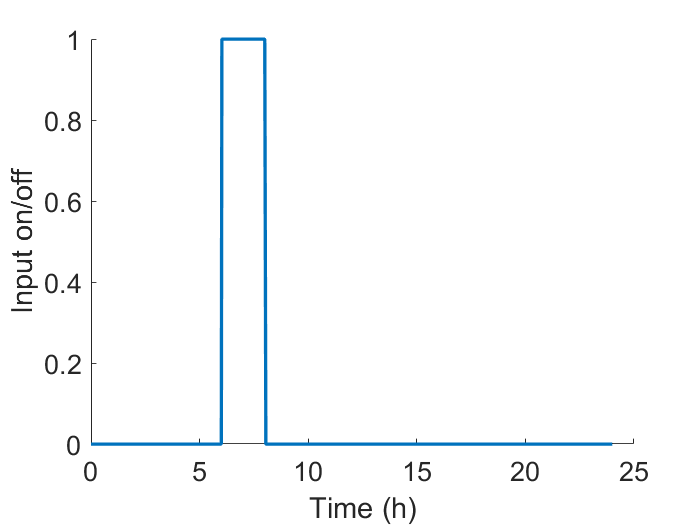
\includegraphics[width=\textwidth]{figure/paper 1/input.png}
		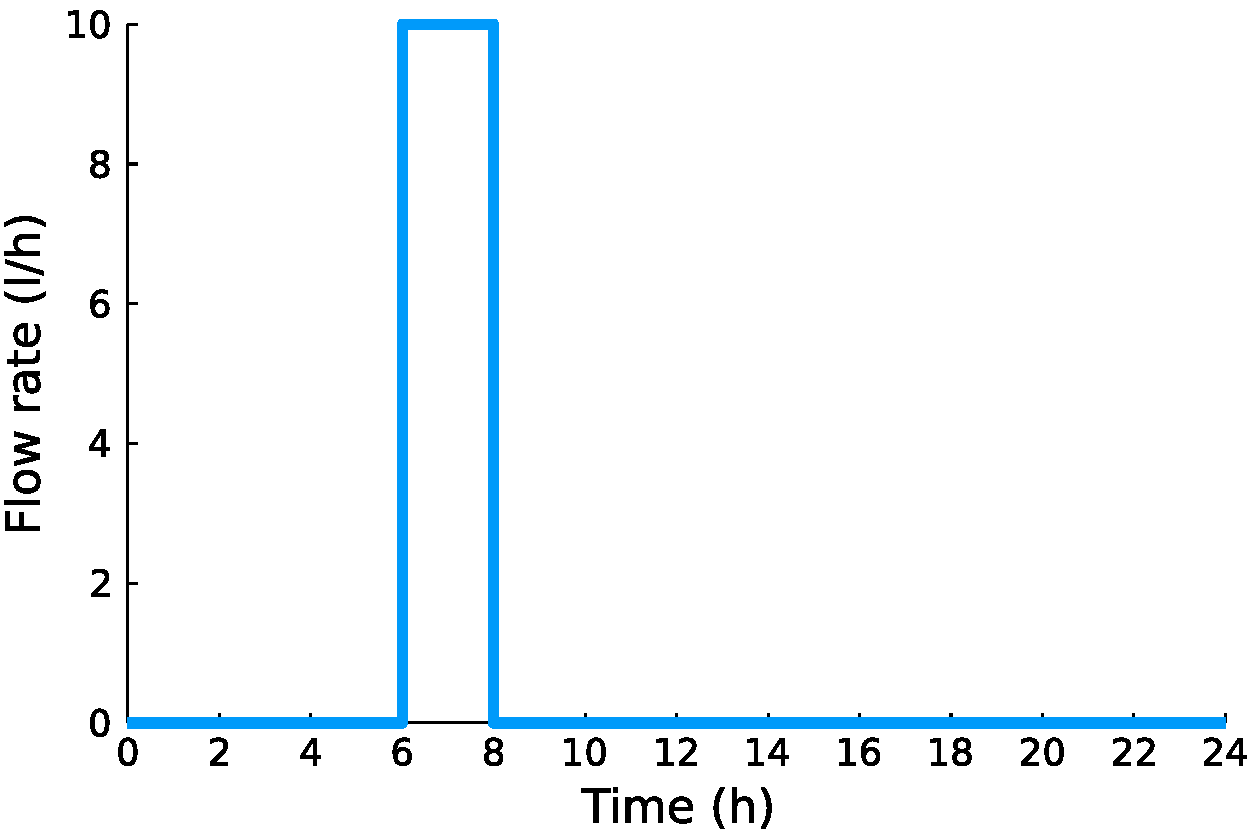
\includegraphics[width=\textwidth]{figure/paper 1/extra1}
		\caption{Optimal $\text{O}_2$ input profile.}
		\label{input1}
	\end{subfigure}
	~ %add desired spacing between images, e. g. ~, \quad, \qquad, \hfill etc. 
	%(or a blank line to force the subfigure onto a new line)
	\begin{subfigure}[b]{0.45\textwidth}
		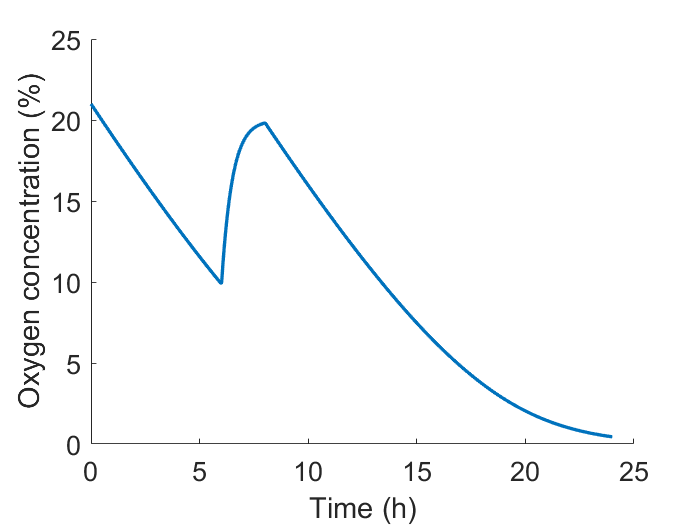
\includegraphics[width=\textwidth]{figure/paper 1/design.png}
		\caption{$\text{O}_2$ concentration in the jar.}
		\label{output1}
	\end{subfigure}
	\caption{Optimal design, assuming $l=2$ and $n=12$: pulse input after $6 \text{ h}$.}
	\label{figODE1}
\end{figure}
\begin{figure}
	\centering
	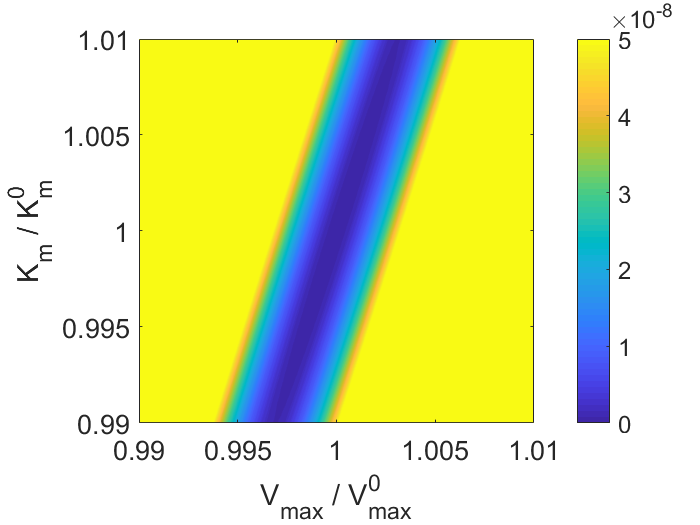
\includegraphics[width=0.8\textwidth]{figure/paper 1/compare1.png}
	\caption{SSE contours for the optimal design in Figure \ref{input1}.}
	\label{figCompare1}
\end{figure}
\\
\\
While a full enumeration of the design space was feasible for our proof of concept example, we also tested the performance of the initial and the modified coordinate-exchange algorithm. In each case, we ran the algorithm $10,000$ times. When applying the initial algorithm, the optimal experiment was found only ten times. So, while this simple algorithm performs well for response surface models, it is clearly not appropriate for our dynamical models, with our specific parametrization of the $\text{O}_2$ input profile. When applying the modified algorithm, we obtained the global optimum in $1,014$ of the $10,000$ iterations of the algorithm, a considerable improvement.
\subsubsection{Comparison to benchmark designs}
We now compare the first optimal experimental design of Figure \ref{input1} to four intuitive benchmark designs, also considered in the full enumerative search. More specifically, we provide a comparison with two constant input profiles, a maximally dynamic profile and an alternative pulse. Table \ref{table1} lists these benchmark designs and their D-criterion values.
\begin{table}
	\centering
	\begin{tabular}{|c|c|}
		\hline 
		Experimental design & D-criterion \\ 
		\hline 
		Optimal design: pulse after $6 \text{ h}$& $3.56\e{15}$  \\ 
		
		Alternative design: Always on & $9.37\e{7}$ \\ 
		
		Alternative design: Always off & $2.66\e{15}$ \\ 
		
		Alternative design: Switching on/off & $2.64\e{11}$ \\ 
		
		Alternative design: pulse after $4 \text{ h}$ & 
		$3.16\e{15}$ \\ 
		\hline
	\end{tabular} 
	\caption{D-criterion values for both the optimal design as well as several benchmarks, assuming $l=2$ and $n=12$. {\color{red}These designs are shown in Figures \ref{figODE1} --- \ref{compare4}.}} 
	\label{table1}
\end{table}
\\
\\
We also performed a detailed graphical comparison by calculating the squared error identification functional in Equation (\ref{F}) for different parameter vectors, in the neighborhood of the initial parameter vector $\mathbf{p}^0$. If other parameters would fit the system almost equally well, the sum of squared errors (SSE) would not vary substantially in the neighborhood of the initial parameters values, suggesting imprecise parameter estimation. The SSE contours resulting from the first optimal experimental design are shown in Figure \ref{figCompare1}. All values larger than the maximum on the color bar are displayed in the same yellow color as the maximum itself. The values on the axes are relative to the initial parameter values. The function is steep in the vertical and horizontal direction, indicating precise parameter estimates. However, the principal axes of the ellipses are not parallel with the horizontal and vertical axes, and the contours are elongated diagonally. This indicates that even the optimal experimental design would result in correlated parameter estimates. In other words, the two parameters cannot be estimated independently. This is a well-known problem when estimating Michaelis-Menten models.
\\
\\
Figure \ref{SSEcompare2} depicts the SSE contours resulting from the constant input profile that continuously pumps air into the jar, for the full duration of the experiment in Figure \ref{inputcompare2}. The D-criterion corresponding to that experimental design is much lower, $9.37\e{7}$. As a result, this benchmark experiment performs considerably worse in terms of the quality of the estimates than the optimal design in Figure \ref{figODE1}: the SSE value is insensitive to the values of the parameters $K_\text{m}$ and $V_{\text{max}}$.
\\
\\
The other constant input profile we considered as a benchmark and which is shown in Figure \ref{inputcompareLiterature}, is the always off profile. This profile has a D-criterion value much closer to that of the optimal design, namely $2.66\e{15}$. The resulting contours for the SSE value are shown in Figure \ref{SSEcompareLiterature}, and resemble those in Figure \ref{figCompare1}. However, they have a slightly larger surface area.
\\
\\
Figure \ref{compare3} demonstrates that the SSE contours produced by a maximally dynamic input profile are quite different from the contours produced by the optimal design. The maximally dynamic profile switches input every $2 \text{ h}$ and the D-criterion value equals $2.64\e{11}$, for that profile. This demonstrates that optimal dynamic design of experiments is not equivalent to changing the input as frequently as possible.
\\
\\
In Figure \ref{compare4}, we show a pulse input function that occurs $2 \text{ h}$ earlier than the pulse in the optimal experimental design, as well as the SSE contours corresponding to that input. This profile performs much better than the other benchmark experimental designs. This is also reflected in the D-criterion value of $3.16\e{15}$, which shows that designs that are close to the optimal design are also similar in information content.
\begin{figure}[H]
	\centering
	\begin{subfigure}[b]{0.45\textwidth}
		%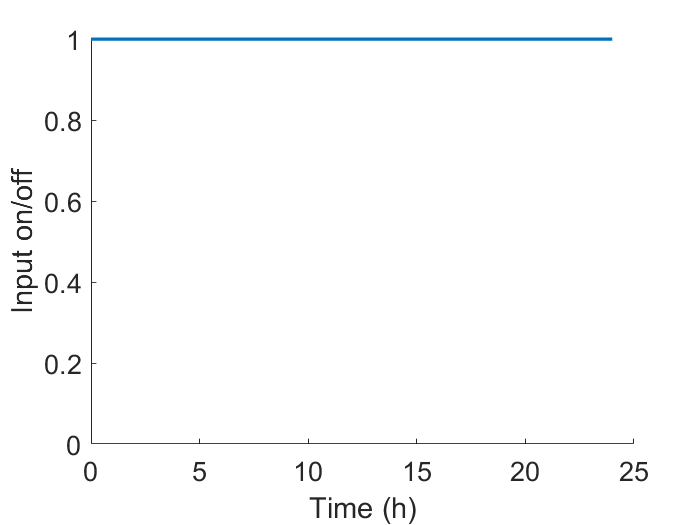
\includegraphics[width=\textwidth]{figure/paper 1/compare2input.png}
		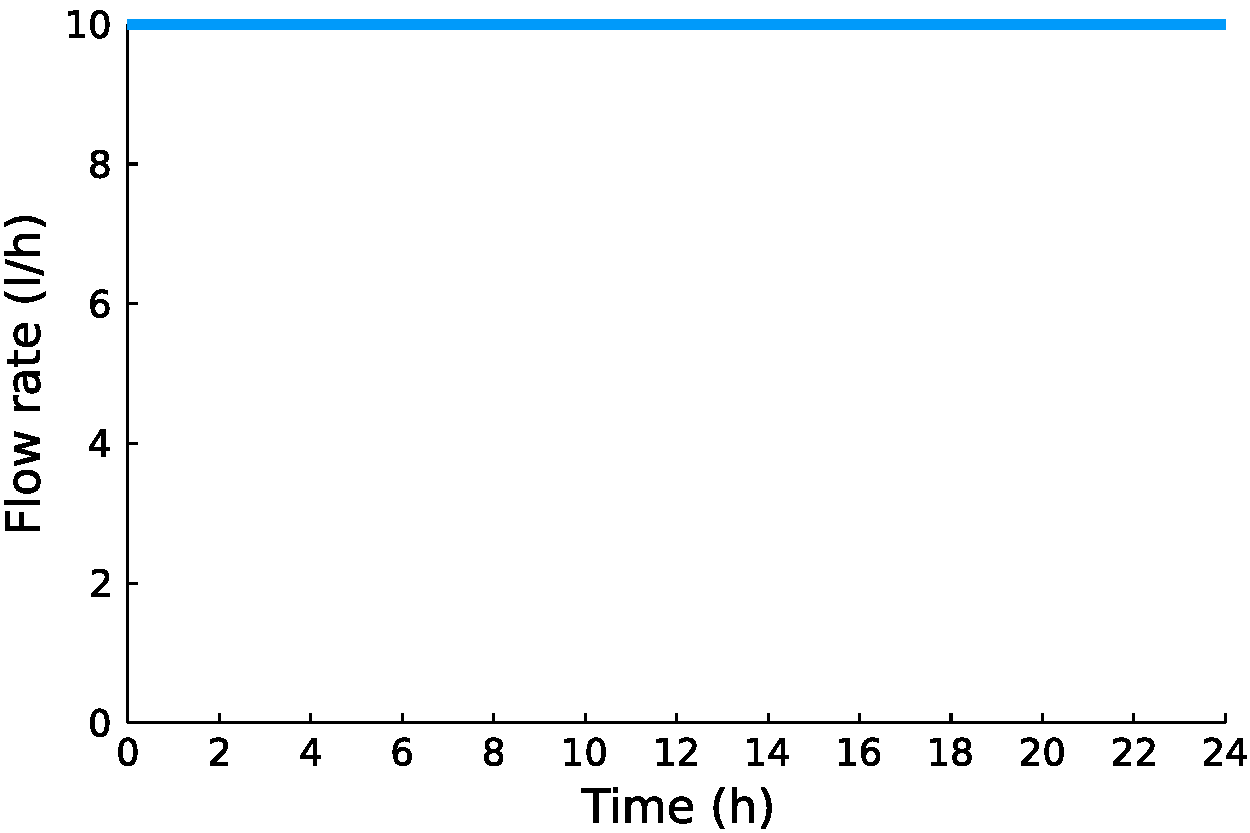
\includegraphics[width=\textwidth]{figure/paper 1/extra2}
		\caption{Oxygen input profile.}
		\label{inputcompare2}
	\end{subfigure}
	~ %add desired spacing between images, e. g. ~, \quad, \qquad, \hfill etc. 
	%(or a blank line to force the subfigure onto a new line)
	\begin{subfigure}[b]{0.45\textwidth}
		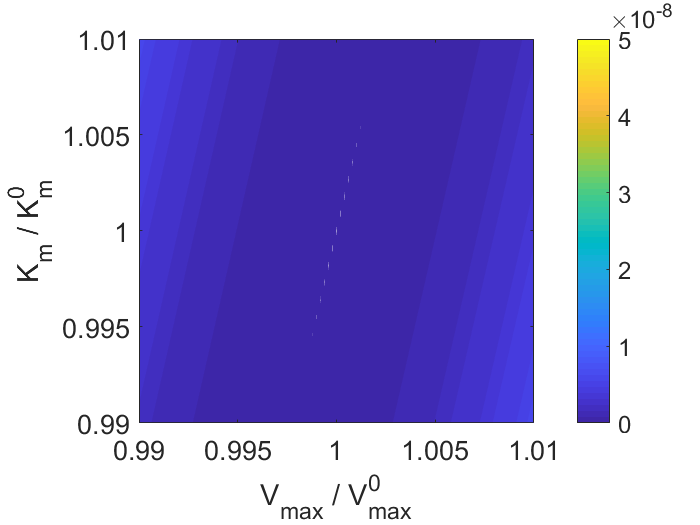
\includegraphics[width=\textwidth]{figure/paper 1/compare2.png}
		\caption{SSE contours.}
		\label{SSEcompare2}
	\end{subfigure}
	\caption{First benchmark: an always-on input profile.}
	\label{compare2}
\end{figure}
\begin{figure}[H]
	\centering
	\begin{subfigure}[b]{0.45\textwidth}
		%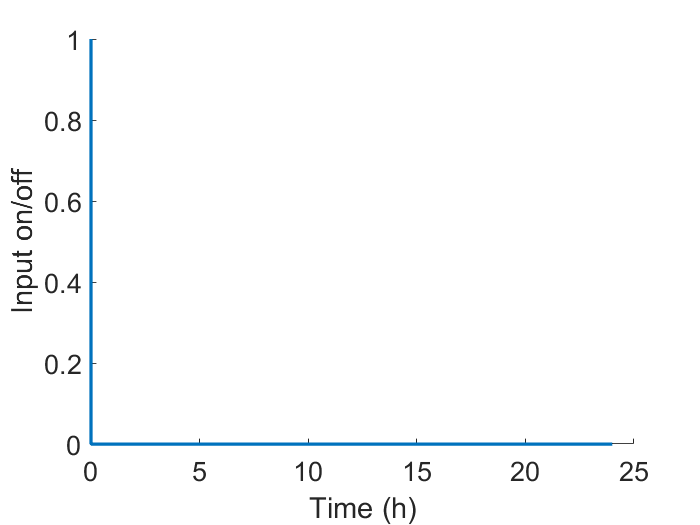
\includegraphics[width=\textwidth]{figure/paper 1/inputLiterature.png}
		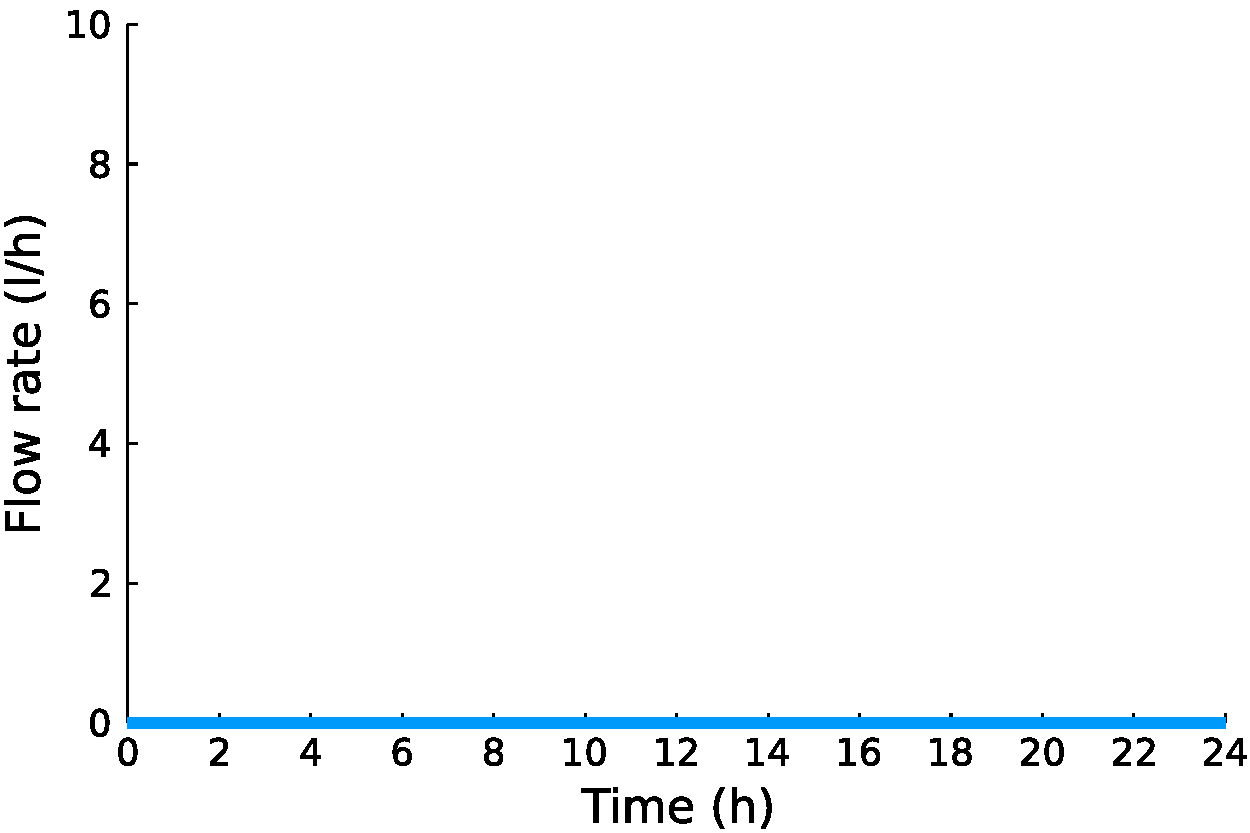
\includegraphics[width=\textwidth]{figure/paper 1/extra3}
		\caption{Oxygen input profile.}
		\label{inputcompareLiterature}
	\end{subfigure}
	~ %add desired spacing between images, e. g. ~, \quad, \qquad, \hfill etc. 
	%(or a blank line to force the subfigure onto a new line)
	\begin{subfigure}[b]{0.45\textwidth}
		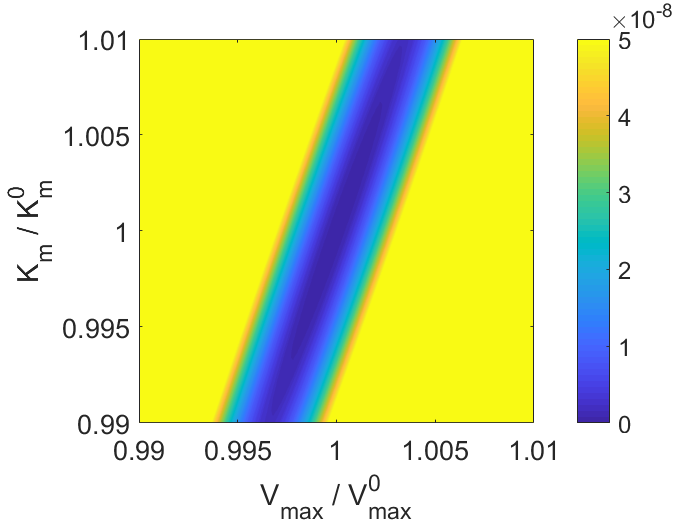
\includegraphics[width=\textwidth]{figure/paper 1/compareLiterature.png}
		\caption{SSE contours.}
		\label{SSEcompareLiterature}
	\end{subfigure}
	\caption{Second benchmark: an always-off input profile.}
	\label{compareLiterature}
\end{figure}
\begin{figure}[H]
	\centering
	\begin{subfigure}[b]{0.45\textwidth}
		%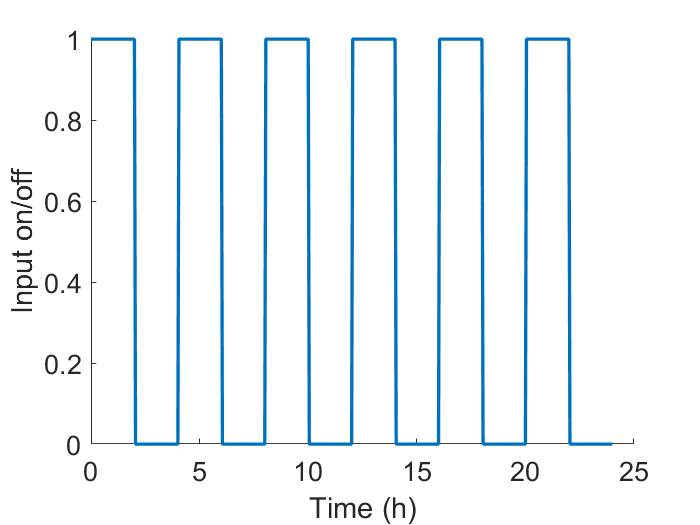
\includegraphics[width=\textwidth]{figure/paper 1/compare3input.png}
		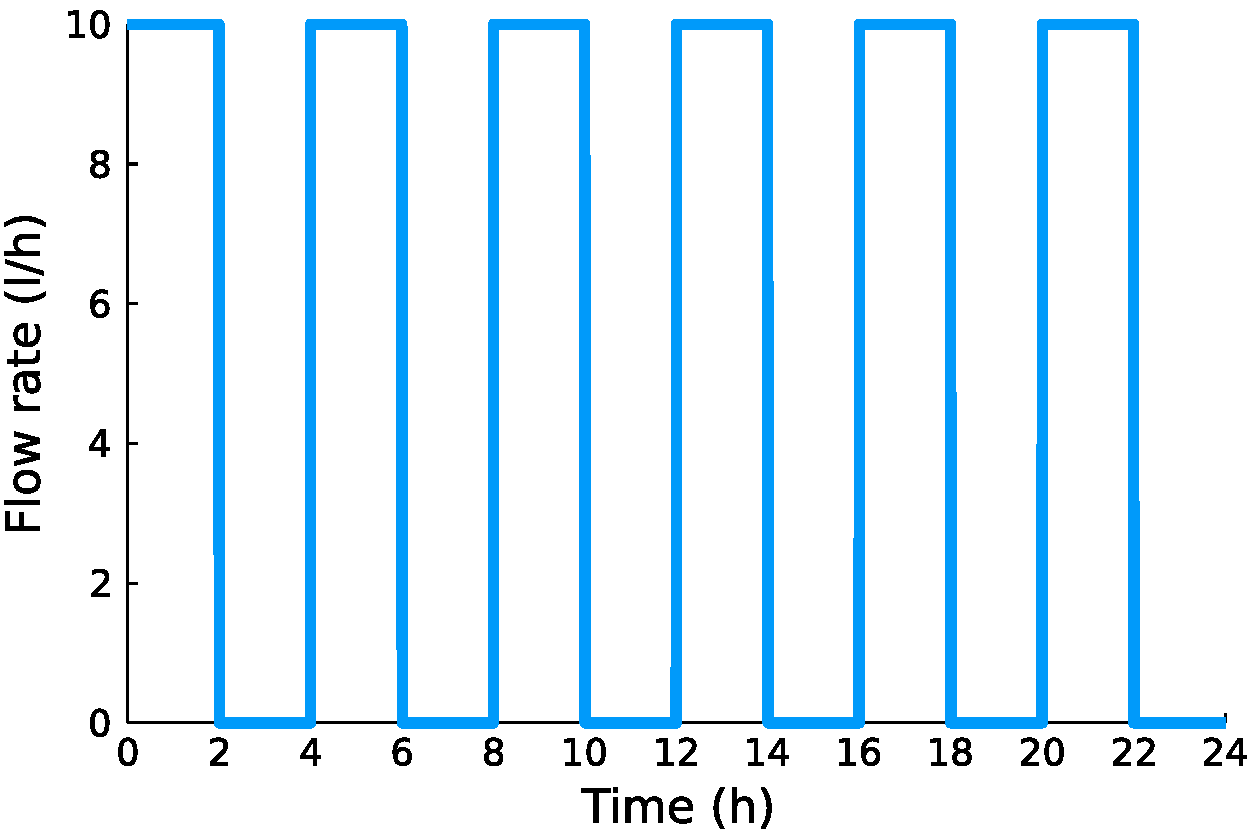
\includegraphics[width=\textwidth]{figure/paper 1/extra4}
		\caption{Oxygen input profile.}
		\label{inputcompare3}
	\end{subfigure}
	~ %add desired spacing between images, e. g. ~, \quad, \qquad, \hfill etc. 
	%(or a blank line to force the subfigure onto a new line)
	\begin{subfigure}[b]{0.45\textwidth}
		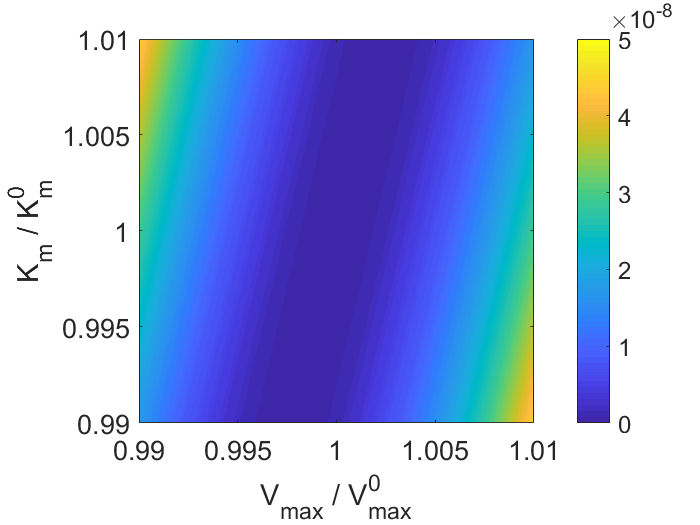
\includegraphics[width=\textwidth]{figure/paper 1/compare3.png}
		\caption{SSE contours.}
		\label{SSEcompare3}
	\end{subfigure}
	\caption{Third benchmark: a constantly switching input profile.}
	\label{compare3}
\end{figure}
\begin{figure}[H]
	\centering
	\begin{subfigure}[b]{0.45\textwidth}
		%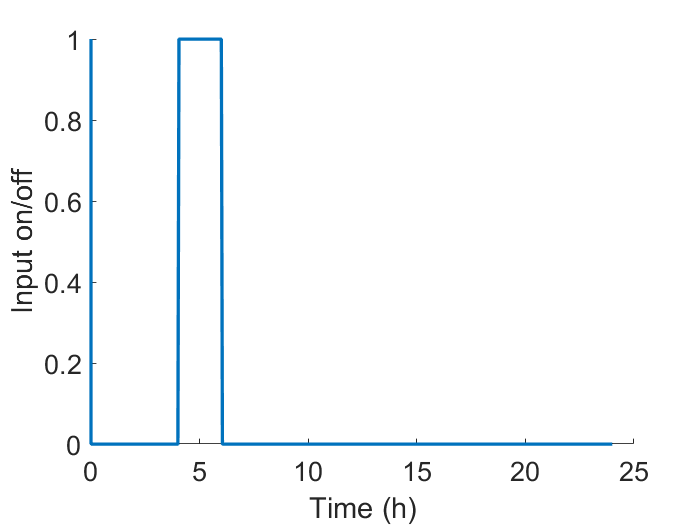
\includegraphics[width=\textwidth]{figure/paper 1/compare4input.png}
		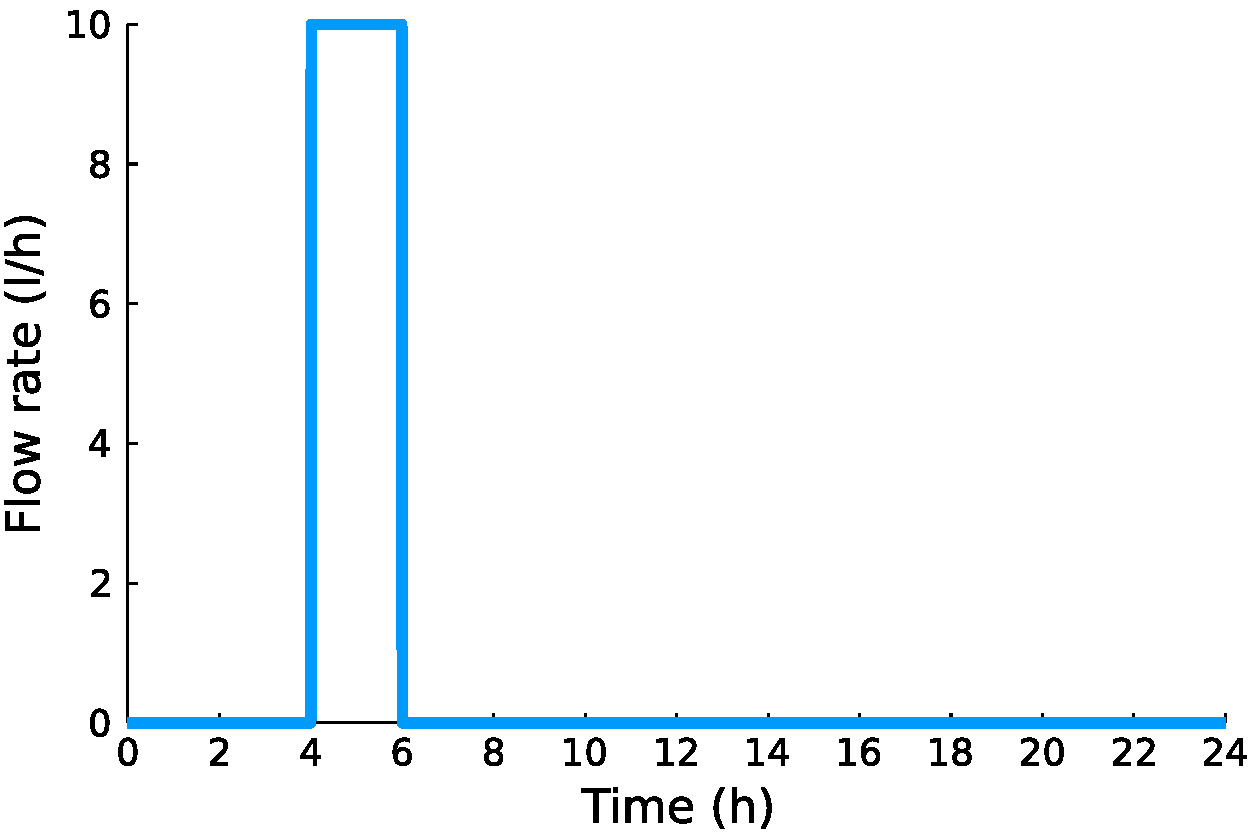
\includegraphics[width=\textwidth]{figure/paper 1/extra5}
		\caption{Oxygen input profile.}
		\label{inputcompare4}
	\end{subfigure}
	~ %add desired spacing between images, e. g. ~, \quad, \qquad, \hfill etc. 
	%(or a blank line to force the subfigure onto a new line)
	\begin{subfigure}[b]{0.45\textwidth}
		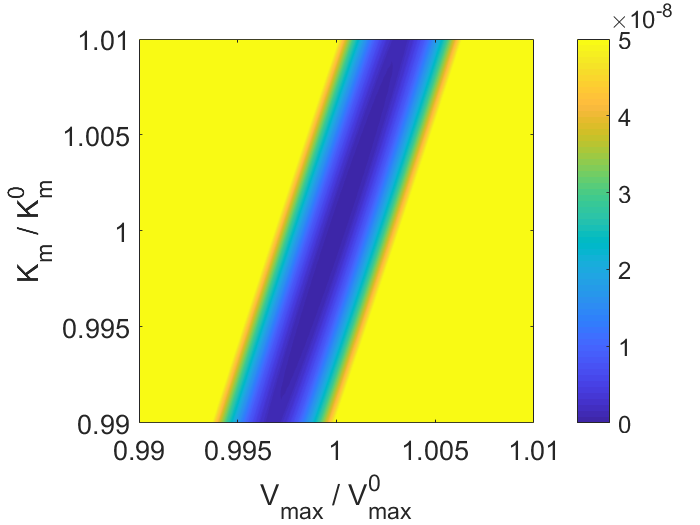
\includegraphics[width=\textwidth]{figure/paper 1/compare4.png}
		\caption{SSE contours}
		\label{SSEcompare4}
	\end{subfigure}
	\caption{Fourth benchmark: pulse input after $4 \text{ h}$.}
	\label{compare4}
\end{figure}
\subsection{Refining the Design Space}
We refined the parametrization of the proof of concept experimental designs in two different ways. The D-criterion values of the optimal input profiles are listed in Table \ref{table2}.
\label{Refinement}
\begin{table}
	\centering
	\begin{tabular}{|c|c|}
		\hline 
		Optimal experimental design & D-criterion \\ 
		\hline 
		$n = 12$ and $l = 2$& $3.56\e{15}$  \\ 
		
		$n = 144$ and $l = 2$& {\color{red}$5.15\e{17}$ }\\ 
		
		$n = 12$ and $l= 11$& {\color{red}$5.13\e{17}$} \\ 
		\hline
	\end{tabular} 
	\caption{D-criterion values for optimal experimental designs with different parametrizations  in Sections \ref{Experiment2} and \ref{Experiment3}. {\color{red}These designs are shown in Figures \ref{figODE1}, \ref{figODE2} and \ref{figODE3}.}} 
	\label{table2}
\end{table}

\subsubsection{Allowing more frequent input changes}
\label{Experiment2}
For the construction of our second optimal experimental design, we allowed the inputs to be changed every $10 \text{ min}$, instead of every $2 \text{ h}$, while still only allowing an on or off input. As all admissible input profiles from the proof of concept example are also admissible under the new settings, the second optimal design problem generalizes the initial one, since $120 \text{ min}$ is divisible by $10 \text{ min}$. The set of admissible input profiles in our second optimal design problem can thus be considered as a refinement of the first. To identify the optimal experimental design for the new problem, we used $10, 000$ iterations of the modified coordinate-exchange algorithm. The unique best design found by the modified coordinate-exchange algorithm is depicted in Figure \ref{input2}. It was found in 45 of the $10, 000$ iterations of the algorithm and involves two short $10 \text{ min}$ pulses during the second half of the experiment. The resulting $\text{O}_2$ concentration in the jar is shown in Figure \ref{output2}. The D-criterion value of this design amounts to {\color{red}$5.15\e{17}$}, which is much better than the value of the optimal design in the proof of concept example.
\begin{figure}
	\centering
	\begin{subfigure}[b]{0.45\textwidth}
		%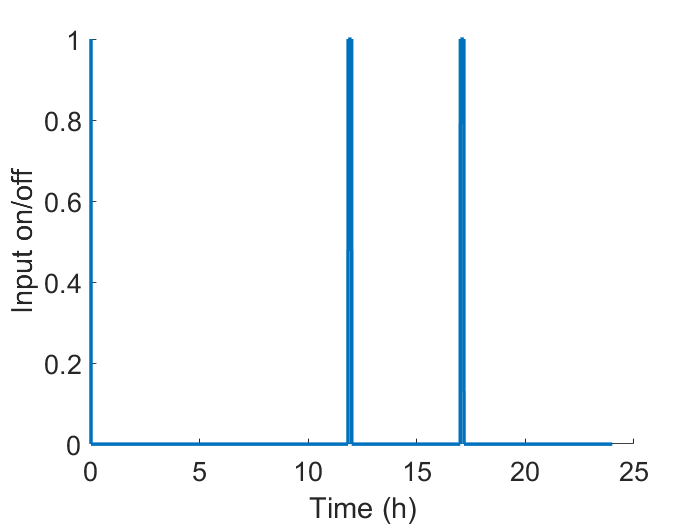
\includegraphics[width=\textwidth]{figure/paper 1/input2.png}
		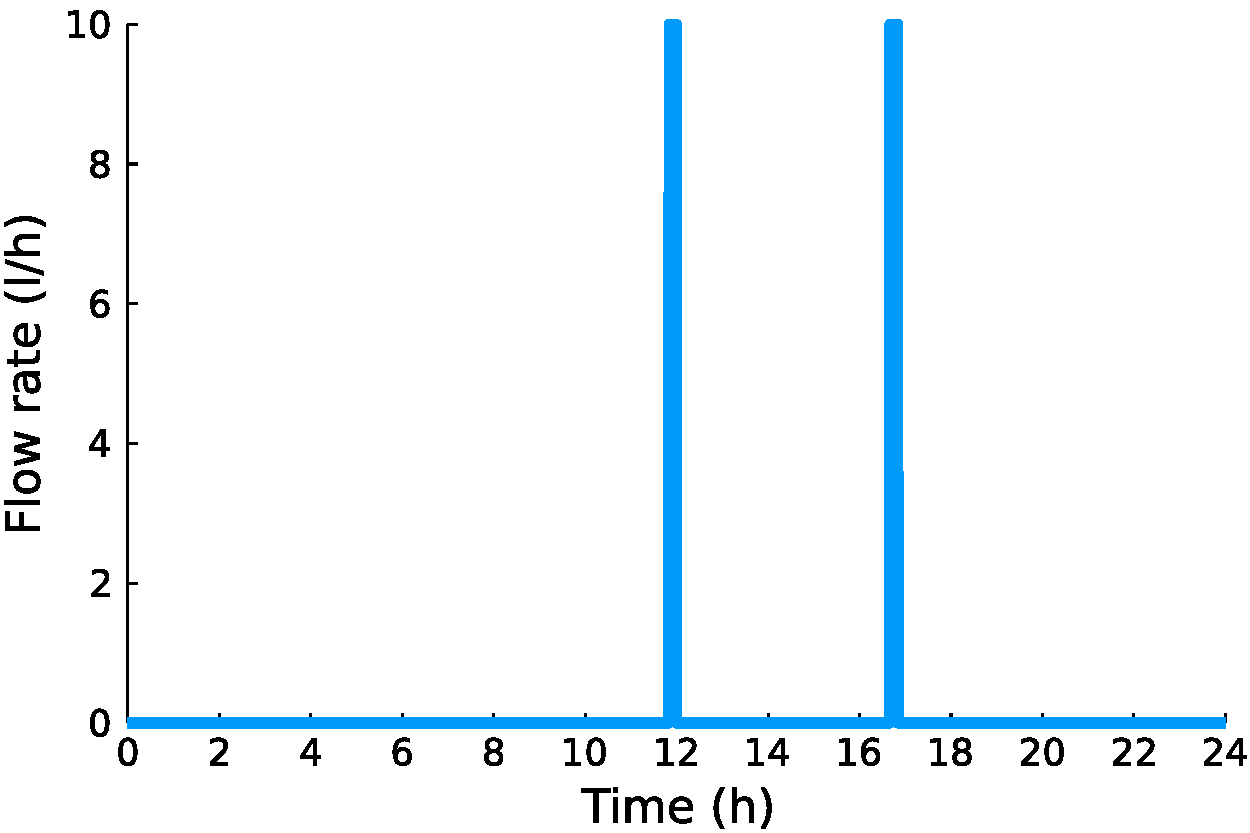
\includegraphics[width=\textwidth]{figure/paper 1/extra6}
		\caption{$\text{O}_2$ input profile.}
		\label{input2}
	\end{subfigure}
	~ %add desired spacing between images, e. g. ~, \quad, \qquad, \hfill etc. 
	%(or a blank line to force the subfigure onto a new line)
	\begin{subfigure}[b]{0.45\textwidth}
		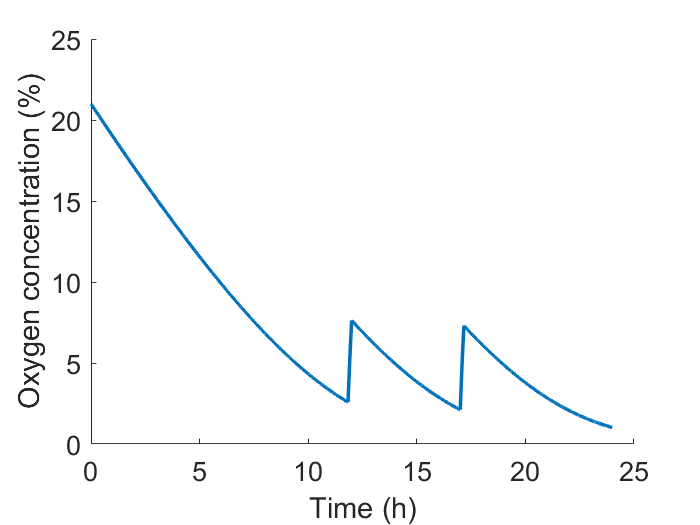
\includegraphics[width=\textwidth]{figure/paper 1/design2.png}
		\caption{$\text{O}_2$ concentration in the jar.}
		\label{output2}
	\end{subfigure}
	\caption{Optimal design, assuming $l=2$ and $n=144$: two short pulses during the second half of the experiment.}
	\label{figODE2}
\end{figure}
\\
\\
The new optimal profile differs substantially from the first in Figure \ref{input1}: instead of one longer pulse from $6 \text{ to } 8 \text{ h}$, two shorter $10 \text{ min}$ pulses after $12 \text{ and } 17 \text{ h}$ are preferred. The reason why this design is optimal is, however, very similar to that of the previous example. After an initial decrease, the $\text{O}_2$ concentration in the jar keeps hovering around the value of the Michaelis-Menten constant $K_\text{m}$, providing information about the switching behavior of the system between saturated and linear respiration. If the $\text{O}_2$ concentration would drop even lower, little respiration would occur and thus little information would be gained concerning the two model parameters. The preference for two short pulses over one longer pulse can be explained by comparing Figure \ref{figODE2} to Figure \ref{output1}. A longer pulse increases the $\text{O}_2$ concentration in the jar almost to the initial one. Since the system always starts at atmospheric conditions, information about maximal respiration is always present in the initial phase of the experiment. Returning to that high concentration does not yield new information. Instead, there is added value in studying the respiration at concentrations around $K_\text{m}$. Therefore, the optimal profile involving two shorter pulses focuses more on the switching behavior instead of revisiting the region of saturated respiration.
\subsubsection{Allowing more input levels}
\label{Experiment3}
In our final optimization, we allowed the input to take 11 different levels, equally spaced between the maximum and minimum input level. The input was only allowed to be changed every $2 \text{ h}$, unlike in the previous example. Again, all possible designs encountered during the first optimization, were considered in this third optimization problem. So, this example also generalizes the proof of concept example. The unique best design found using $10,000$ iterations of the modified coordinate-exchange algorithm, is depicted in Figure \ref{input3}. That input profile was found in 75 of the 10,000 iterations. The corresponding $\text{O}_2$ concentration in the jar is shown in Figure \ref{output3}. The D-criterion value of {\color{red}$5.13\e{17}$} is very similar to that of the input profile in Figure \ref{input2}, as can be seen in Table \ref{table2}.
\begin{figure}
	\centering
	\begin{subfigure}[b]{0.45\textwidth}
		%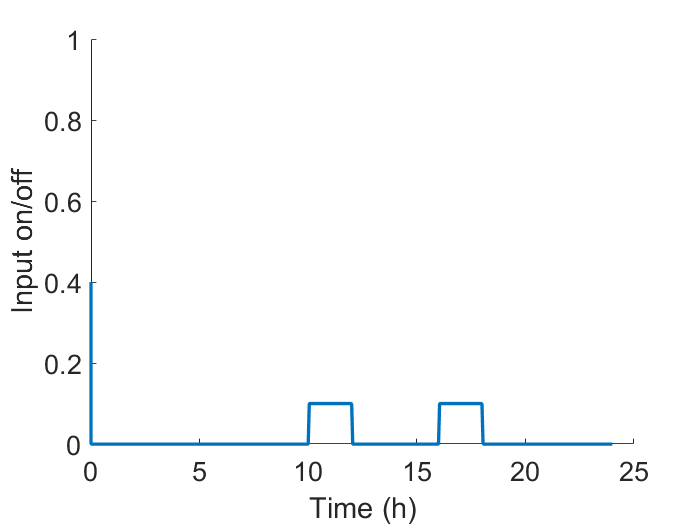
\includegraphics[width=\textwidth]{figure/paper 1/input3.png}
		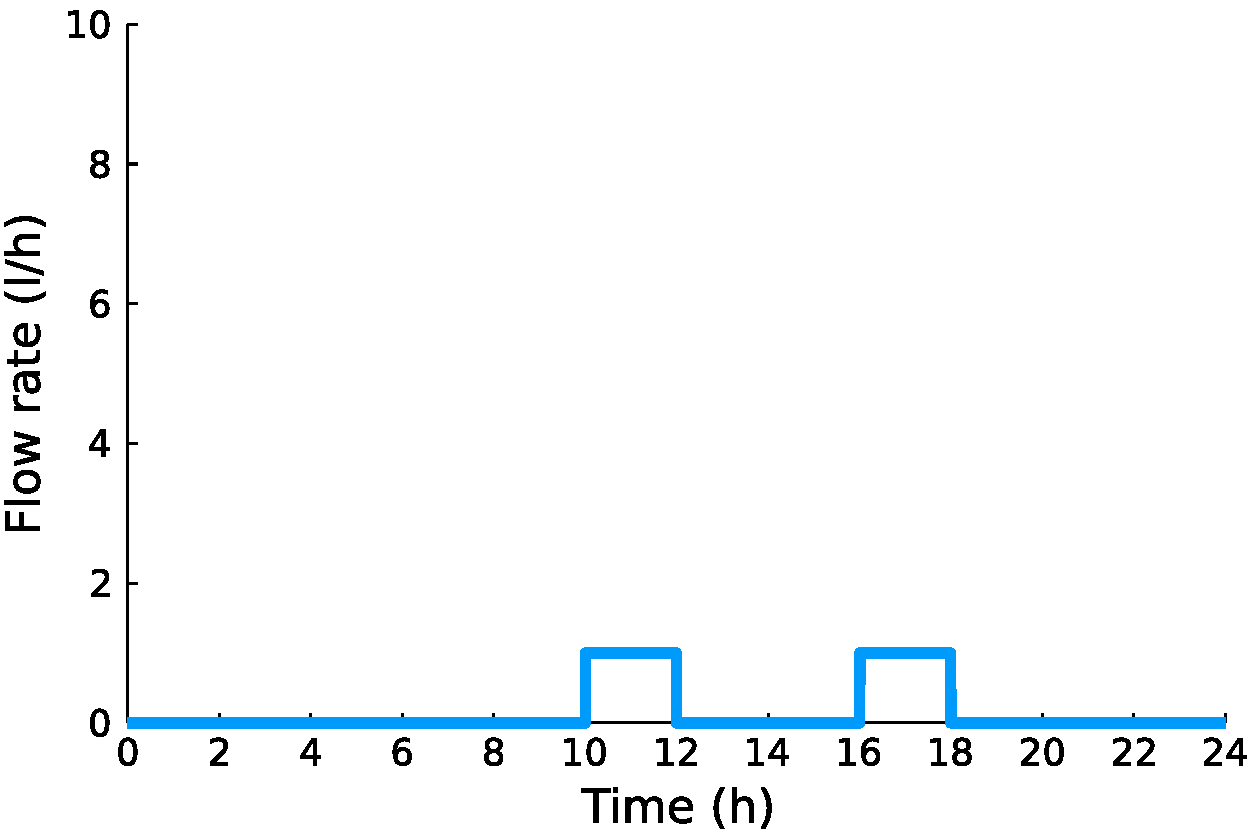
\includegraphics[width=\textwidth]{figure/paper 1/extra7}
		\caption{Optimal $\text{O}_2$ input profile.}
		\label{input3}
	\end{subfigure}
	~ %add desired spacing between images, e. g. ~, \quad, \qquad, \hfill etc. 
	%(or a blank line to force the subfigure onto a new line)
	\begin{subfigure}[b]{0.45\textwidth}
		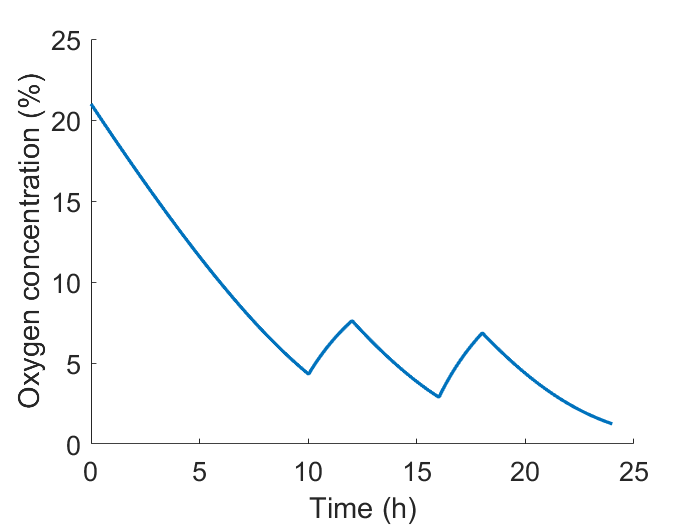
\includegraphics[width=\textwidth]{figure/paper 1/design3.png}
		\caption{$\text{O}_2$ concentration in the jar.}
		\label{output3}
	\end{subfigure}
	\caption{Optimal design, assuming $l = 11$ and $n = 12$: two small pulses after $10 \text{ h}$ and $16 \text{ h}$.}
	\label{figODE3}
\end{figure}
\\
\\
A similar dynamic input, consisting of two pulses, seems to be preferred in the last two examples. In the third, experiment the small pulses take the minimum non-zero input value of $0.1$, or $10$ $\%$ of the maximum allowed flow rate. The simulated outlet $\text{O}_2$ concentrations shown on Figure\ref{output2} and Figure \ref{output3}, look remarkably similar, which shows that even with different parametrizations of the input curve, a similar dynamic behavior can be achieved.
\\
\\
The SSE contours in Figure \ref{figCompare5} correspond to the input profiles of Figure \ref{input2} and Figure \ref{input3}. As already noted, the designs involve similar dynamic $\text{O}_2$ concentration trends, have similar D-criterion values and thus also have very similar contour plots. The contours in Figure \ref{figCompare5} are also much steeper than those in Figure \ref{figCompare1}, but they are still elongated diagonally. So, even a refinement of the design space did not help to remove the correlation between the two parameter estimates.
\begin{figure}
	\centering
	\begin{subfigure}[b]{0.45\textwidth}
		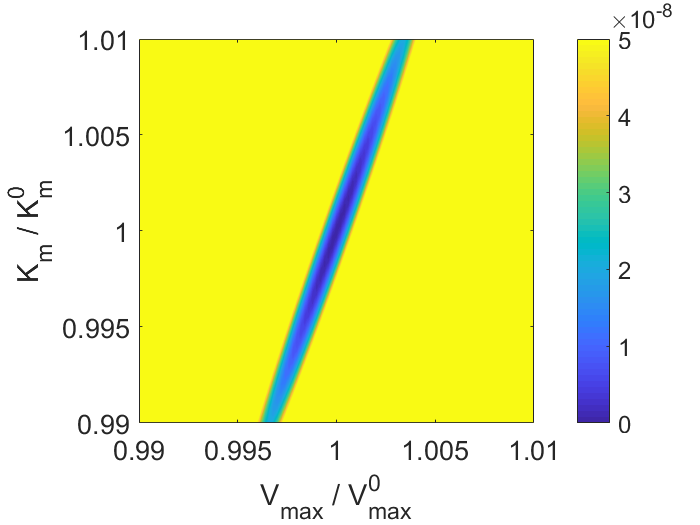
\includegraphics[width=\textwidth]{figure/paper 1/compare5.png}
		\caption{Optimal design in Figure \ref{input2}.}
		\label{SSEopt2}
	\end{subfigure}
	~ %add desired spacing between images, e. g. ~, \quad, \qquad, \hfill etc. 
	%(or a blank line to force the subfigure onto a new line)
	\begin{subfigure}[b]{0.45\textwidth}
		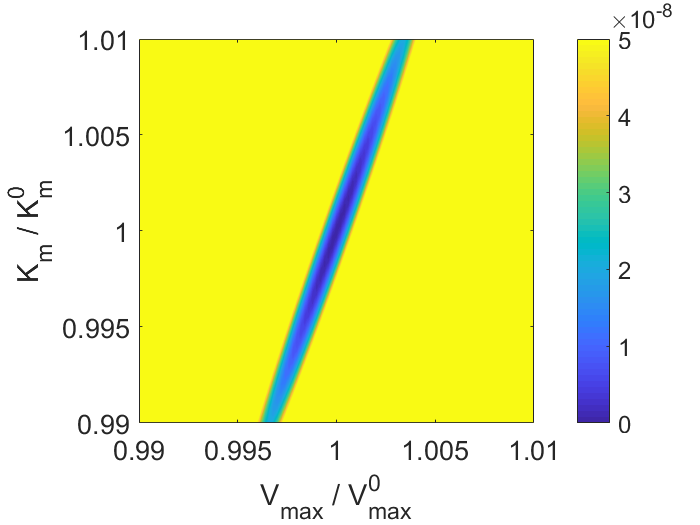
\includegraphics[width=\textwidth]{figure/paper 1/compare6.png}
		\caption{Optimal design in Figure \ref{input3}.}
		\label{SSEopt3}
	\end{subfigure}
	\caption{SSE contours for the optimal experimental designs in Figure \ref{input2} and \ref{input3}.}
	\label{figCompare5}
\end{figure}
\section{Discussion}
\label{Discussion}
{\color{red}In Section \ref{Information}, we mentioned that several design optimality criteria have been proposed in literature. We opted for the D-criterion because it does not depend on the chosen units to describe the model, unlike other criteria such as the A-optimality criterion, which minimizes the average variance of the parameter estimates.} Another criterion that is independent from the chosen units is the I-optimality criterion, which seeks to minimize the average prediction variance over the family of all admissible input profiles {\color{red} \parencite{goos1}}. However, this criterion is computationally more expensive than the D-criterion, which, combined with the already computationally intensive dynamic experimental design idea, would lead to prohibitively long computation times.
\\
\\
In this chapter, we calculated locally optimal designs for a given set of initial values $\mathbf{p}^0$.  Most of the literature on design of experiments for non-linear models focuses on locally optimal design \parencite{fedorov}. This is especially so in the dynamic case \parencite{bernaerts1,bernaerts2,balsa1,balsa2,nahor1,nahor2}. However, we often possess more a priori information concerning a parameter than just a point estimate. For instance, we might also have access to a confidence interval for each model parameter. We could also incorporate this information into our design, with a technique called Bayesian optimal design \parencite{chaloner}, at the expense of a substantial amount of computing time. 
\\
\\
In this chapter, we considered input profiles that are practically feasible. More specifically, when determining the first optimal experimental design, we parametrized our input profile, as a function that could only be on or off. These kinds of input profiles can be easily implemented in practice. We improved on this first design in two different ways: by allowing more than two input levels, and by allowing the input to be switched more rapidly. Similar gains in information were achieved by both improvements, so that there is flexibility in how to perform an informative experiment.
\\
\\
In most of the existing literature, as well as in this chapter, only a single input profile has been optimized \parencite{bernaerts1,bernaerts2,balsa1,balsa2,nahor1,nahor2}. A useful extension of this work would be to optimize multiple input profiles at the same time. Another interesting avenue for future research would be to optimize input profiles for estimating distributed parameter models, which describe the dynamical system by partial differential equations, instead of our lumped approach, which uses ordinary differential equations. {\color{red}The assumption of perfect mixing can then also be relaxed.} Examples of such models are the reaction-diffusion models developed by \textcite{tri2}. To optimize input profiles for such models, however, we first need to develop measures for quantifying parameter uncertainty in these models and for quantifying the information content of the experiments used for collecting the data required for model estimation. (As is often the case in statistics and data science, model development is ahead of tools to verify model quality \parencite{efronhastie}.)
\section{Conclusion}
This chapter presented a pioneering study about the usefulness of optimal dynamic experiments for non-linear modeling in postharvest research. Three D-optimal dynamic experimental designs for the estimation of the Michaelis-Menten respiration parameters of Conference pear were constructed. Each design was constructed using a different parametrization of the input profiles.
\\
\\
The design of protocols for controlled or modified atmosphere of fruit and vegetables is increasingly based on dynamical models of their respiration. Successful implementation depends on accurate knowledge of the model parameters, since every fruit cultivar has to be stored under slightly different conditions. Determining all these conditions is a labor-intensive activity, and requires efficient experimentation. Our three optimal designs show that optimal dynamic design of experiments increases the quality of the respiration parameters' estimates compared to some benchmarks. Therefore, optimal dynamic design of experiments has the potential to facilitate the successful implementation of controlled and modified atmosphere storage. As a matter of fact, dynamic experimentation is a generic method: while our experiments were optimized for Conference pear, a different choice of prior information can be used to obtain optimal input profiles for different cultivars. However, in this chapter, we only took respiration of pear fruit into account. {\color{red}We also used a locally optimal experimental design method which may not be robust. In the next chapter, we improve both these aspects.}
\chapter{Robust Dynamic Experiments for the Precise Estimation of Respiration and Fermentation Parameters of Fruit and Vegetables}
\label{paper2}
This chapter has been written by Arno Strouwen with feedback from Professors Goos and Nicolaï.
\\
\\
{\color{red}Source code available upon request.}
\section*{Abstract}
Dynamic models based on non-linear differential equations are increasingly being used in many biological applications. Highly informative dynamic experiments are valuable for the identification of these dynamic models. The storage of fresh fruit and vegetables is one such application where dynamic experimentation is gaining momentum. In this chapter, we construct optimal $\oxy$ and $\coxy$ gas input profiles to estimate the respiration and fermentation kinetics of pear fruit. The optimal input profiles, however, depend on the true values of the respiration and fermentation parameters. Locally optimal design of input profiles, which uses a single initial guess for the parameters, is the traditional method to deal with this issue. This method, however, is very sensitive to the initial values selected for the model parameters. Therefore, we suggest a Bayesian experimental design approach to robustify our input profiles to the unknown values of the parameters.
\section{Introduction}
Model-based approaches are commonly used in the analysis, control and optimization of biological systems. These models rely on knowledge of physical, chemical and biological laws, such as mass balances, transport phenomena and reaction kinetics, and are often described by a system of non-linear differential equations, with inputs and outputs. So, often, the structure of a model can be determined from first principles. However, the model will generally also rely on parameters whose numerical values cannot be determined from physical laws. These parameters must then be inferred from experimental data before the model can be put to use. The experiments required to estimate these parameters are often laborious and cost prohibitive. It is therefore important to determine experimental conditions that are rich in information and thus allow a precise estimation of the unknown model parameters.
\\
\\
At present, the model parameters are often estimated from data collected using multiple experiments at various combinations of input levels, which are kept constant throughout each individual experiment. Even if an appropriate experimental design technique is used to reduce the number of experiments that have to be performed, the experimental effort remains considerable. Alternatively, experiments in which the inputs vary in time can be conducted. This has been shown to be a cost-effective way to generate a highly informative data set \parencite{versyck}. Such experiments are called dynamic. In optimal design of dynamic experiments, time-varying input profiles are constructed to optimize the information content of a single experiment.
\\
\\
The major challenge for experimental design for any non-linear model is the dependence of the optimal input profiles on the true values of the unknown model parameters, whose estimation is the primary goal of the experiment. This dependence is due to the non-linearity of the model. Most of the experimental design literature uses a scalar function of the Fisher information matrix as the measure of information content in an experiment, as this matrix is inversely related to the covariance matrix of the model parameters. An informative experiment thus ensures a small covariance matrix of the model parameters. Locally optimal design of input profiles uses initial guesses for the model parameters to calculate this information matrix \parencite{fedorov}. This method has already been used to construct informative time-varying inputs in chemical engineering \parencite{franceschini} and in biological fields such as systems biology \parencite{balsa1}, predictive microbiology \parencite{bernaerts1,bernaerts2} and food engineering \parencite{balsa2,nahor}. However, an input profile that is highly informative for one set of parameter values may lack information for other parameter values. Thus, if the initial guesses {\color{red}for} the parameters differ substantially from the true values, then the {\color{red}locally optimal design} might not allow precise parameter estimates. So, locally optimal design is sensitive to the initial parameter guesses and is thus not robust {\color{red}\parencite{asprey}}.
\\
\\
Much recent research in experimental design for non-linear models aims at robustifying the design to the true, but unknown, values of the model parameters. A robust design provides a large information content regardless of the true values of these parameters. For dynamic experiments, in particular, a min-max based approach has been used by \textcite{bauer, korkel}. Here, the design is optimized for a worst case scenario. Fisher information matrices are calculated for a set of possible parameter values and the experiment is scored based on the least informative matrix in this set. In contrast, an expected value approach is taken by \textcite{schenkendorf, telen, nimmegeers}. In this approach, the average information content of the experiments over all possible parameter values is optimized. The expected value approach tends to perform better for a large subset of probable parameter values than the min-max approach, but not for extreme sets of parameter values. The expected value approach is also called Bayesian experimental design, because the possible parameter values can be expressed using a prior distribution \parencite{chaloner}. The expected value approaches of \textcite{telen, nimmegeers} rely on  parametric distributions to describe the uncertainty on the model parameters before the experiment has taken place. However, a parametric distribution will often not be appropriate to fully quantify the uncertainty on the model parameters, {\color{red}as we show in the examples in this chapter}. Therefore, in this chapter, we allow arbitrary distributions to quantify the model parameter uncertainty. More specifically, we show how the results of a Bayesian analysis of historical data using Markov-chain Monte-Carlo can be used as a prior distribution. This Markov chain can then be used to calculate the average Fisher information matrix, and has the advantage that it can represent arbitrary distributions \parencite{gelman}.               
\\
\\
Postharvest storage of fresh fruit and vegetables is one biological application where optimal experimental design is useful. The ideal storage temperature as well as $\oxy$ and $\coxy$ partial pressures depend on the respiration characteristics, which in turn depend on species, cultivar, ripeness and multiple other factors. Determining the ideal storage conditions therefore requires much experimentation. Traditionally, this was done by independently storing the product at many different combinations of temperature as well as $\oxy$ and $\coxy$ partial pressures, and by monitoring the respiration and fermentation \parencite{saltveit}. Many modern storage applications, such as modified atmosphere packaging \parencite{fonseca} and dynamic controlled atmosphere \parencite{bessemans}, adopt a model-based approach, where the product is described as a dynamic system with inputs and outputs. The resulting models enable us to use the tools of optimal dynamic experimental design to construct informative experiments. The respiration and fermentation kinetics are generally described by a model of the Michaelis-Menten type \parencite{hertog}. Robust experimental design is particularly needed for postharvest applications because of the large biological variability of fresh fruit and vegetables. As a consequence of that variability, the parameters of the aforementioned kinetic models vary substantially between seasons and origins {\color{red}\parencite{tri}}. In this chapter, we therefore focus on constructing robust experimental techniques to estimate the respiration and fermentation kinetics of pear fruit. This chapter describes the first use of robust optimal experimental design techniques in postharvest research.
\\
\\
This chapter is structured as follows. First, in Section \ref{sec_OED}, we present our robust experimental design methodology. Next, in Section \ref{sec_pear}, we present a state of the art dynamic respiration and fermentation model for pear fruit, and quantify the initial uncertainty on the model parameters using a Markov-chain Monte-Carlo analysis of a prior data-set from \textcite{ho}. In Section \ref{sec_experiments}, we construct both locally and Bayesian optimal designs for this model. Finally, in Section \ref{sec_discussion}, we end with a discussion of alternative techniques.
\section{Bayesian Optimal Experimental Design for Dynamical Systems}
\label{sec_OED}
In this section, we first present the type of dynamical models considered in this chapter. Then, we show how to quantify the information gained from measurements, using the Fisher information matrix. Next, we discuss how to maximize this information content using appropriate control inputs. Finally, we explain how to make the optimal control inputs robust.
\subsection{Dynamic Models}
In this chapter, we consider experimental design for dynamic models of the form:
\begin{equation}
\label{systemP2}
\begin{aligned}
\frac{\dd \bm x}{\dd t} &= f(t,\bm x,\bm \theta,\bm u(t)), \qquad \text{with } \bm x(t=0) = \bm x_0;\\
\bm y_k &= h(\bm x(t_k)) + \bm \epsilon_k,
\end{aligned}
\end{equation}
where $t$ denotes the time ranging from $0$ to $t_e$, the end time of the experiment. The column vector $\bm y_k$ contains the measurements taken at time point $t_k$, with $k$ ranging from $1$ to $N$, the number of measurement times. The time between measurements is equally spread, so that $t_k = \nicefrac{kt_e}{N}$. A measurement at the end of the experiment is thus included, but not at the start. The measurements are subject to independent zero mean Gaussian noise. More specifically,  $\bm \epsilon_k$ is identically and independently multivarate normally distributed with zero mean and covariance matrix $\bm R$. The measurements depend on the dynamic state column vector $ \bm x(t)$ through the measurement function $h$. The states $\bm x(t)$ have to be calculated from the system of ordinary differential equations $f$, with initial conditions $\bm x_0$. This system depends on the unknown model parameter column vector $\bm \theta$, and the controllable input column vector $\bm u(t)$.
\subsection{Information Content of an Experiment}
\label{secFIM2}
Our goal is to optimize the controllable inputs $\bm u(t)$ so that the measurements $\bm y_k$ contain as much information as possible about the unknown parameters $\bm \theta$. A popular way to quantify the information content is the Fisher information matrix (FIM) \parencite{fedorov, walter}:
\begin{equation}
\mathbb{F}(\bm \theta, \bm u(t))= \sum_{k=1}^N
\frac{\partial \bm x(t_k)}{\partial \bm \theta}^T
\frac{\partial h}{\partial \bm x}^T
\bm R^{-1}
\frac{\partial h}{\partial \bm x}
\frac{\partial \bm x(t_k)}{\partial \bm \theta}.
\label{FIM}
\end{equation}
The sensitivities of the states to the unknown parameters, $\nicefrac{\partial \bm x(t_k)}{\partial \bm \theta}$, cannot be computed directly, as the evolution over time of the states $\bm x(t)$ is described by the system of differential equations in Equation (\ref{systemP2}). However, these sensitivities can be calculated from the forward sensitivity differential equations:
\begin{equation}
\frac{\dd}{\dd t} \frac{\partial \bm x}{\partial \bm \theta}
=  \frac{\partial}{\partial \bm \theta}\frac{\dd \bm x}{\dd t}
= \frac{\partial f}{\partial \bm x}\frac{\partial \bm x}{\partial \bm \theta}
+ \frac{\partial f}{\partial \bm \theta},
\qquad \text{with } \frac{\partial \bm x(t=0)}{\partial \bm \theta} = \bm 0.
\label{sens}
\end{equation}
The FIM is the inverse of the Cramer-Rao lower bound of the variance of an unbiased estimator of $\bm \theta$. This lower bound can be interpreted geometrically as a hyper-ellipsoid defined by the eigenvectors and the inverse of the eigenvalues of the FIM. We want this lower bound to be as small as possible, and thus the eigenvalues of the FIM to be as large as possible, because this implies precise estimates for $\bm \theta$ are possible. {\color{red}Several scalar functions have been proposed to} quantify the size of the FIM \parencite{atkinson}. In our work, we use the determinant of the FIM, also called the D-optimality criterion. This criterion is inversely related to the volume of the hyper-ellipsoids, measuring the uncertainty about the parameter vector $\bm \theta$.
\subsection{Discretizing the Controls}
Optimal experimental design for dynamic systems is an infinite dimensional optimization problem since it requires finding optimal controls $\bm u(t)$ for every $t \in [0,t_e]$. To make this problem tractable, the controls have to be discretized in time. We utilize a bounded piecewise constant discretization allowing $\bm u(t)$ to switch values at $M$ equally spaced time points,
\begin{equation}
\bm u_{\min} \leq \bm u(t) = \sum_{j=1}^M \bm u_j \chi_{\left [\nicefrac{(j-1)t_e}{M},\nicefrac{jt_e}{M}\right [ }(t) \leq \bm u_{\max},
\label{input}
\end{equation}
where $\bm u_j$ is the constant control vector during the interval
$\left [\nicefrac{(j-1)t_e}{M},\nicefrac{jt_e}{M}\right [$, and $\chi_A$
is the indicator function,
\begin{equation}
\chi_A(t) =
\begin{cases} 1 \quad t\in A \\ 0 \quad t\not\in A, \end{cases}
\end{equation}
and $\bm u_{\min}$ and $\bm u_{\max}$ are the minimum and maximum control values allowed. Piecewise constant input profiles do not only have the benefit of making our optimization problem tractable, but they are also easy to implement in practice.
\subsection{Robustifying the Experiment}
Another issue with experimental design for models that are non-linear in the parameter vector $\bm \theta$, such as the model we described in Equation (\ref{systemP2}), is the dependence of the FIM on $\bm \theta$. This presents us with a cyclic problem because we are performing the experiment to quantify those parameters. Locally optimal experimental design is the traditional method to deal with this issue. In this approach, the FIM is calculated using a single initial guess $\bm \theta^*$ obtained from any available prior knowledge. A locally optimal experimental design is thus given by:
\begin{equation}
\argmax_{\bm u_1 \ldots \bm u_M} \quad \left | \mathbb{F}(\bm \theta^*, \bm u(t)) \right |
\qquad \text{subject to } \bm u_{\min} \leq \bm u(t) \leq \bm u_{\max}.
\label{localD}
\end{equation}
This method might give poor results if the initial guess deviates from the true value, and is thus not robust. Bayesian optimal design offers a solution to this robustness problem by averaging the information content of the experiment over multiple possible values of the parameters, taking into account the likelihood of each parameter value. More specifically, a weighted average is used to quantify the information content, where the weights are given by a prior distribution of the parameters $p(\bm \theta)$. This distribution represents the {\color{red}knowledge} of uncertainty concerning these parameters, before the experiment has been performed. A robust experimental design is therefore given by:
\begin{equation}
\argmax_{\bm u_1 \ldots \bm u_M} \quad \int \left | \mathbb{F}(\bm \theta, \bm u(t)) \right | p(\bm \theta) \dd \bm \theta
\qquad \text{subject to } \bm u_{\min} \leq \bm u(t) \leq \bm u_{\max}.
\label{pseudoD}
\end{equation}
This criterion is also called the Bayesian D-optimality criterion \parencite{chaloner}, because of the use of a prior distribution.
\\
\\
Generally, the integral in Equation (\ref{pseudoD}) cannot be evaluated analytically. To approximate it numerically, we draw $R$ random model parameter vectors, $\bm \theta_r$, from the prior $p(\bm \theta)$ and average the D-criterion over these values:
\begin{equation}
\label{pseudoDcalc}
\quad \int \left | \mathbb{F}(\bm \theta, \bm u(t)) \right | p(\bm \theta) \dd \bm \theta
\approx \frac{1}{R} \sum_{r=1}^{R} \left | \mathbb{F}(\bm \theta_{r}, \bm u(t)) \right |
\qquad   \bm \theta_r \sim p(\bm \theta).
\end{equation}
The robust criterion in Equation (\ref{pseudoD}) is thus calculated by averaging the FIM over a sample drawn from the prior distribution. The details of the generation of this sample are explained in Section \ref{sec_markov}. 
\subsection{Numerical Details}
The entire optimization problem was implemented in the Julia programming language \parencite{bezanson}. 
All differential equations were solved using the Tsitouras 5/4 Runge-Kutta method \parencite{tsitouras}, as implemented in OrdinaryDiffEq.jl \parencite{rackauckas}. The piecewise constant control switches were implemented using a periodic callback, provided by DiffEqCallbacks.jl. Note that $\bm u(t_e)$ in Equation \ref{input} is undefined, but this value does not influence the FIM.
\\
\\
Because coding the sensitivity differential equations in (\ref{sens}) by hand is quite laborious and error prone, we calculated them exploiting the automatic differentiation capabilities of DiffEqSensitivity.jl \parencite{rackauckas2}, more specifically its implementation of the discrete forward sensitivity analysis method.
\\
\\
To solve the non-linear optimization problems, we used the box constrained optimization capacities of Optim.jl \parencite{mogensen}, which utilizes a log barrier interior point algorithm \parencite{nocedal}. This method requires the specification of an inner solver, for which we used the Broyden–Fletcher–Goldfarb–Shanno (BFGS) algorithm, as also implemented in Optim.jl. The required gradients for this method are calculated by the nested differentiation capabilities of ForwardDiff.jl \parencite{revels}. This interior point optimization method requires an initial experimental design to improve upon and is a local optimizer. Thus, it is not guaranteed to find the absolute best experimental design. To deal with this issue, we utilize multiple starts, each with a different initial design. The TikTak global optimization algorithm \parencite{arnoud} can carefully select these initial designs from the design space, using Sobol points. We use $1000$ starts of the interior point optimization method in combination with the TikTak implementation in MultiStartOptimization.jl.
\section{Respiration and Fermentation Model of Pear Fruit}
In this chapter, we apply our robust experimental design methodology to  precisely estimate the respiration and fermentation characteristics of pear fruit. First, we present a respiration and fermentation model of pear fruit inside a jar. We then quantify the initial uncertainty concerning the various parameters in this model using a published data-set.
\label{sec_pear}
\subsection{Model Description}
\begin{figure}
	\centering
	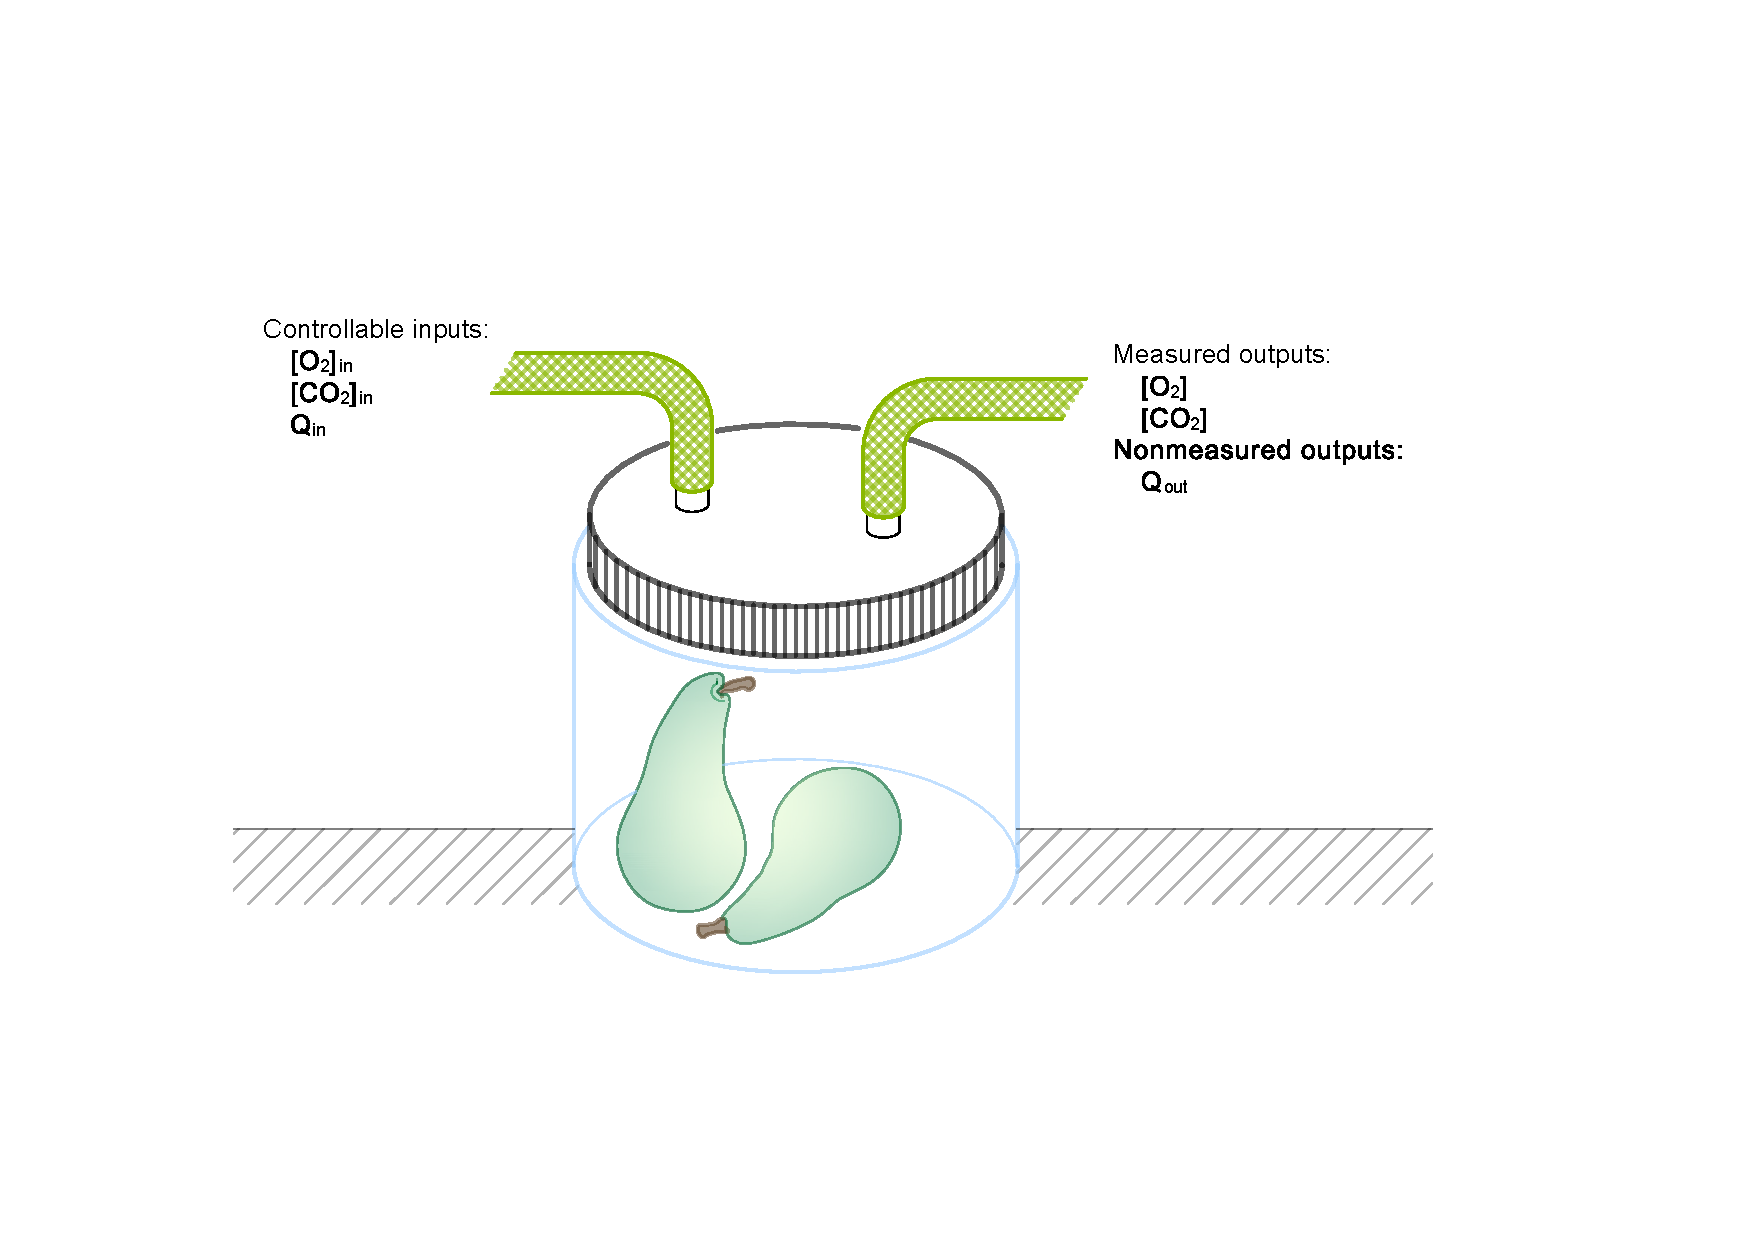
\includegraphics[width=0.9\textwidth,trim={2cm 4cm 2cm 5cm,clip}]{figure/paper 2/pear.pdf}
	\caption{Schematic representation of the measurement setup.}
	\label{figpear}
\end{figure}
\label{sec_model}
The respiration and fermentation of pear fruit inside a jar is modeled by two mass balances for $\oxy$ and $\coxy$:
\begin{equation}
\begin{aligned}
V_\text{j}\diff{\Coxy}{t} &= Q_\text{in}(t)\Coxy_{\text{in}}(t) - Q_\text{out}(t)\Coxy
- m_\text{p}r_{\oxy}(t),\\
V_\text{j}\diff{\Ccoxy}{t} &= Q_\text{in}(t)\Ccoxy_{\text{in}}(t) - Q_\text{out}(t)\Ccoxy
+ m_\text{p}r_{\coxy}(t).
\end{aligned}
\label{respiration}
\end{equation}
The square brackets in these expressions represent concentrations in $\text{mol/m}^3$. These differential equations describe the change of $\oxy$ and $\coxy$ concentrations inside a jar with volume $V_j$, which will equal $5\text{ dm}^3$, in our examples in Section \ref{sec_experiments}. A time varying air mixture with an oxygen concentration $\Coxy_{\text{in}}(t)$ and a carbon dioxide concentration $\Ccoxy_{\text{in}}(t)$ is blown into the jar with flow rate $Q_\text{in}(t)$ (units: $\text{m}^3\text{/h}$). These three time varying functions form the controllable inputs to our system. Our measurement set up is schematically shown in Figure \ref{figpear}.
\\
\\
Since the pressure inside the jar should remain equal to the atmospheric pressure, we can calculate the outflow $Q_\text{out}(t)$ from the jar using the ideal gas law:
\begin{equation}
Q_{\text{out}}(t)\frac{P_\text{atm}}{\bar{R}T} = Q_{\text{in}}\frac{P_\text{atm}}{\bar{R}T} - m_p r_{\oxy}(t) + m_p r_{\coxy}(t),
\label{balance}
\end{equation}
with $\bar{R}$ the universal gas constant and $P_\text{atm}$ the atmospheric pressure. Concentrations throughout the jar and at the outlet are considered to be similar, due to the assumption of well mixing. In the constructed experiments in Section \ref{sec_experiments}, the temperature equals $293.15$ K,  the amount of $\oxy$ consumed and $\coxy$ produced is proportional to the mass of the pears $m_\text{p}$, taken to be 4 kg and the initial conditions for $\oxy$ and $\coxy$ will be equal to regular air.
\\
\\
The respiration rates in Equation (\ref{balance}) are specified using models of the Michaelis-Menten type \parencite{hertog}:
{\color{red}\begin{equation}
\begin{aligned}
r_{\oxy}(t) &= 
\frac{V_{\text{m},\oxy}\Coxy}
{\left(\nicefrac{K_{\text{m},\oxy}}{\bar{R}T} + \Coxy\right)
	\left(1 + \frac{\Ccoxy}{\nicefrac{K_{\text{mn},\text{CO}_2}}{\bar{R}T}}\right)},\\
r_{\coxy}(t) &= 
\text{r}_\text{q}r_{\oxy}(t) + 
\frac{V_{\text{m,f,}\coxy}}
{1 + \frac{\Coxy}{\nicefrac{K_{\text{m,f},\oxy}}{\bar{R}T}}}.
\end{aligned}
\label{inhibitions}
\end{equation}}
The models for these respiration rates contain six parameters that have to be identified. $V_{\text{m},\oxy}$ and $V_{\text{m,f,}\coxy}$ are the maximum respiration and fermentation reaction rates, respectively. The Michaelis-Menten constant $K_{\text{m},\text{O}_2}$ represents the saturation of respiration at high oxygen levels, whereas $K_{\text{mn},\text{CO}_2}$ models the inhibition of respiration by $\coxy$. The respiration quotient $\text{r}_\text{q}$ represents the percentage of $\oxy$ that is converted to $\coxy$ by respiration. Finally, $K_{\text{m,f},\oxy}$ models the inhibition of fermentation by $\oxy$. {\color{red}The three inhibition constants are expressed in units of pressure, which will be required for the analysis in the following section.}
\\
\\
The measured gas concentrations $\Coxy_m$ and $\Ccoxy_m$ at time point $t_k$ are assumed to be equal to the true concentrations plus the additive Gaussian noise terms $\zeta_k$ and $\eta_k$ respectively:
\begin{equation}
\begin{aligned}
\Coxy_{m}(t_k) &= \Coxy(t_k) + \zeta_k,\\
\Ccoxy_{m}(t_k) &= \Ccoxy(t_k) + \eta_k.
\end{aligned}
\end{equation}
Since both measurements are in the same range from $0$ to $30\text{ kPa}$, we assume that the error terms are identically and independently distributed for both outputs, and thus that variance, $\sigma^2$, of the error terms $\zeta_k$ and $\eta_k$ is equal.
{\color{red}Since the two gasses are measured with different sensors, we assume that the two noise terms are independent. Several sensor principles are available for measuring $\oxy$ concentrations in a practical setting, including gas chromatography, zirconium based sensors, paramagnetic sensors and fluorescence based optical sensors; $\coxy$ concentrations can be measured using gas chromatography, infrared absorption and chemical gas sensors.}
\\
\\
{\color{red}Before considering experimental design for this model, we first checked whether the model parameters can be correctly identified at all. This is because it is possible that two different model parameter values result in exactly the same output behavior, making it impossible to distinguish the true value of the model parameters from the data. We confirmed, using the STRIKE-GOLDD Matlab toolbox \parencite{villaverde}, that our respiration and fermentation model is structurally identifiable even with constant input levels, that do not change in time. Our piecewise constant input profiles form a super-set of the set of constant input profiles, which thus ensures that our experimental designs will result in an identifiable model.}
\subsection{Prior Information}
Optimal experimental design for the non-linear model introduced in Section \ref{sec_model} requires prior information, concerning the six respiration and fermentation parameters. Such prior information for pear respiration and fermentation can be found in \textcite{ho}. We cannot directly utilize the published results, as \textcite{ho} only report confidence intervals for each individual parameter, but no correlations between estimates. To deal with this problem, we reanalyzed $50$ time series data-sets, each containing $\oxy$ and $\coxy$ measurements from a single jar, made available to us by the authors. We used a Bayesian data analysis technique to achieve this. More specifically, we utilized a Markov-chain Monte-Carlo method to re-estimate the parameters and quantify the uncertainty in the data  \parencite{betancourt}. The Markov chain stores values sampled from the posterior distribution of the parameters. The chain can thus be utilized for numerically approximating the expectation in the robust criterion in Equation (\ref{pseudoD}). In other words, we use the MCMC chain as an input to the expression in Equation (\ref{pseudoDcalc}).
\\
\\
Because the data of \textcite{ho} were collected at different temperatures, our analysis took into account the effect of temperature on the maximal respiration and fermentation rate by means of the Arrhenius equations:
\begin{equation}
\begin{aligned}
V_{\text{m},\oxy} &=
V_{\text{m},\oxy,T_r}\exp\left(\frac{E_{a,\oxy}}{\bar{R}}\left ( \frac{1}{T_r} - \frac{1}{T} \right) \right),\\
V_{\text{m,f,}\coxy} &= V_{\text{m,f,}\coxy,T_r}\exp\left(\frac{E_{a,\coxy}}{\bar{R}}\left (\frac{1}{T_r} - \frac{1}{T} \right)\right),
\end{aligned}
\end{equation}
where $V_{\text{m},\oxy,T_r}$ and $V_{\text{m,f,}\coxy,T_r}$ are the maximal respiration rates at a reference temperature $T_r$ of $293.15$ K, and $E_{a,\oxy}$ and $E_{a,\coxy}$ are activation energies that describe how the reaction rates increase with the temperature $T$. {\color{red}The different temperatures in the data set influences the inhibition parameters in Equation (\ref{inhibitions}).} These activation energies are nuisance parameters in our computation of optimal input profiles in Section \ref{sec_experiments}, as we only consider experiments at the reference temperature.
\\
\\
{\color{red}Another difference between the experiments of \textcite{ho} and our experiments is that they used closed jars, instead of flow through experiments. Their system dynamics thus differ:
	\begin{equation}
		\begin{aligned}
			V_\text{j}\diff{\Coxy}{t} &= - m_\text{p}r_{\oxy}(t),\\
			V_\text{j}\diff{\Ccoxy}{t} &= m_\text{p}r_{\coxy}(t).
		\end{aligned}
		\label{respirationho}
\end{equation}}
\begin{figure}[t!]
	\centering
	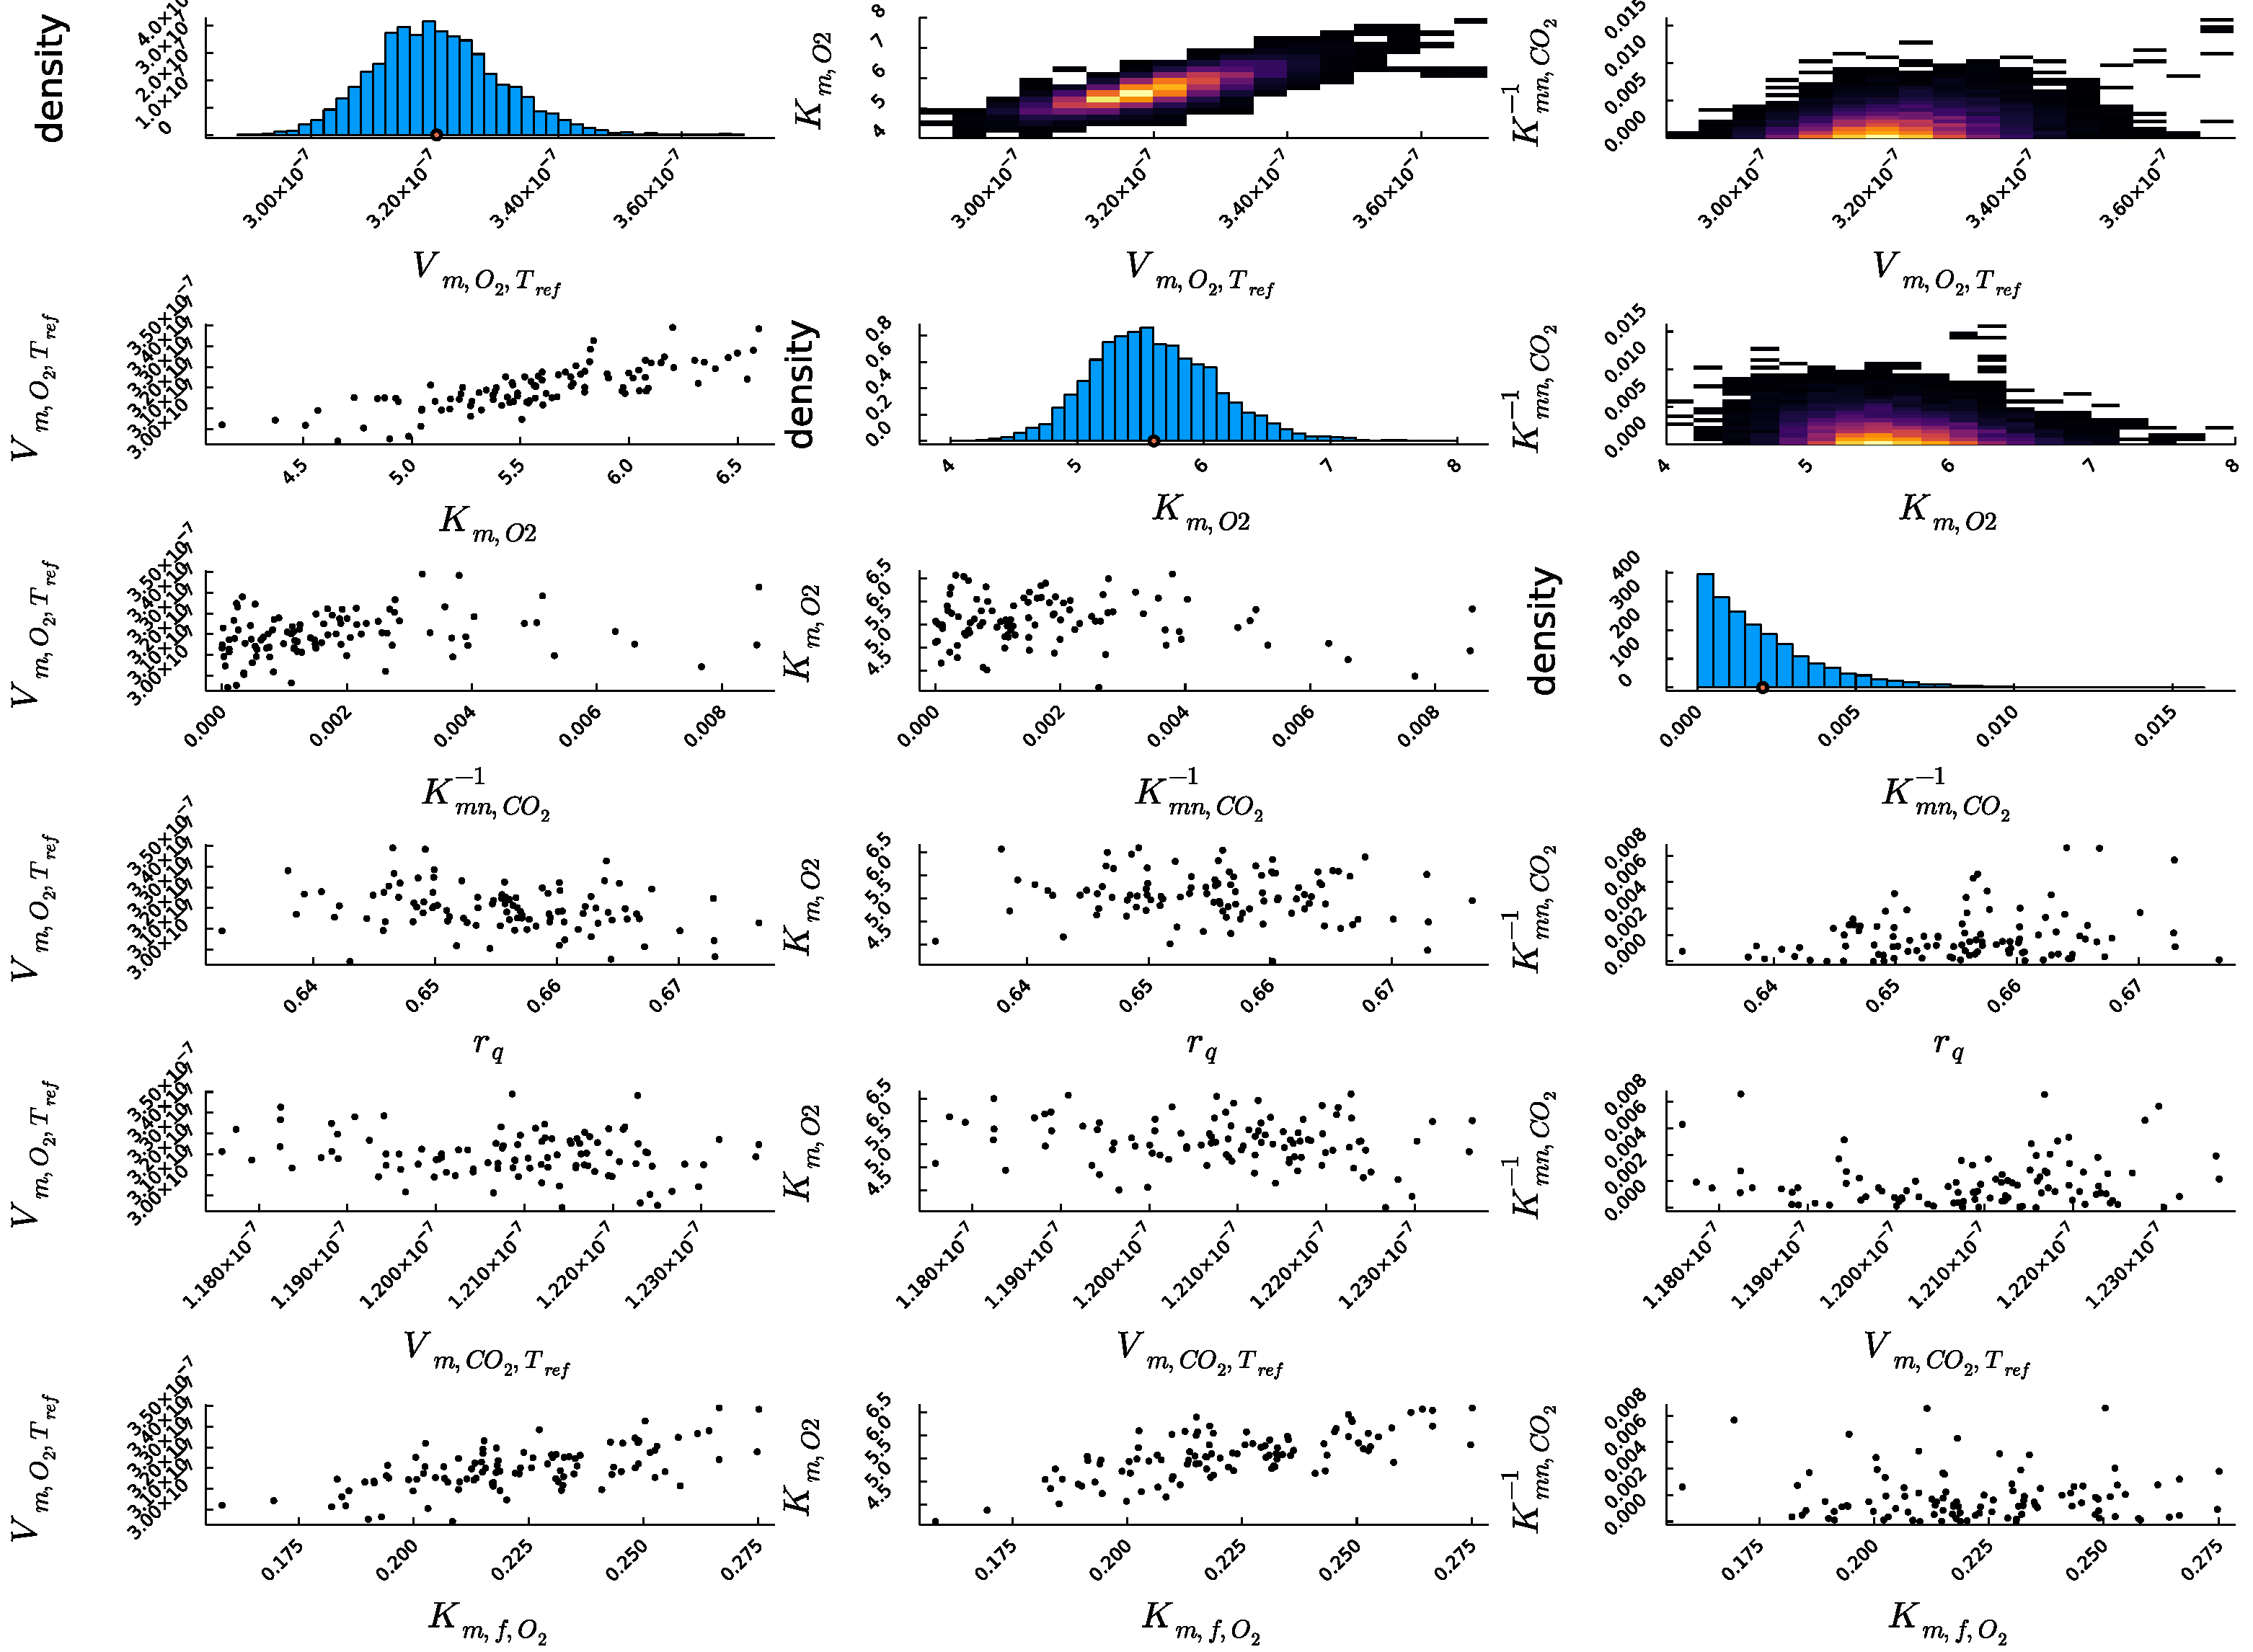
\includegraphics[width=0.99\textwidth]{figure/paper 2/test.pdf}
	\captionsetup{labelformat=empty}
	\caption*{\color{red}This figure is continued on the next page.}
\end{figure}
Figure \ref{figprior} provides a summary of the results of our Bayesian analysis. On the diagonal of this figure, histograms of the Markov chain values of the six model parameters of interest ($V_{\text{m},\oxy}$, $K_{\text{m},\oxy}$, $K_{\text{mn},\text{CO}_2}$, $r_q$, $V_{\text{m,f,}\coxy}$, $K_{\text{m,f},\oxy}$) are shown. Above the diagonal, two-dimensional heatmaps are shown, which visualize the correlation between the Markov chain values for pairs of model parameters. The figures below the diagonal provide similar information, but show only $100$ pairs of values from the Markov chain. Histograms of the Markov chain values for the nuisance parameters $E_{a,\oxy}$, $E_{a,\coxy}$, and $\sigma$ are depicted in Figure \ref{fignuisance}.
\begin{figure}[t!]
	\centering
	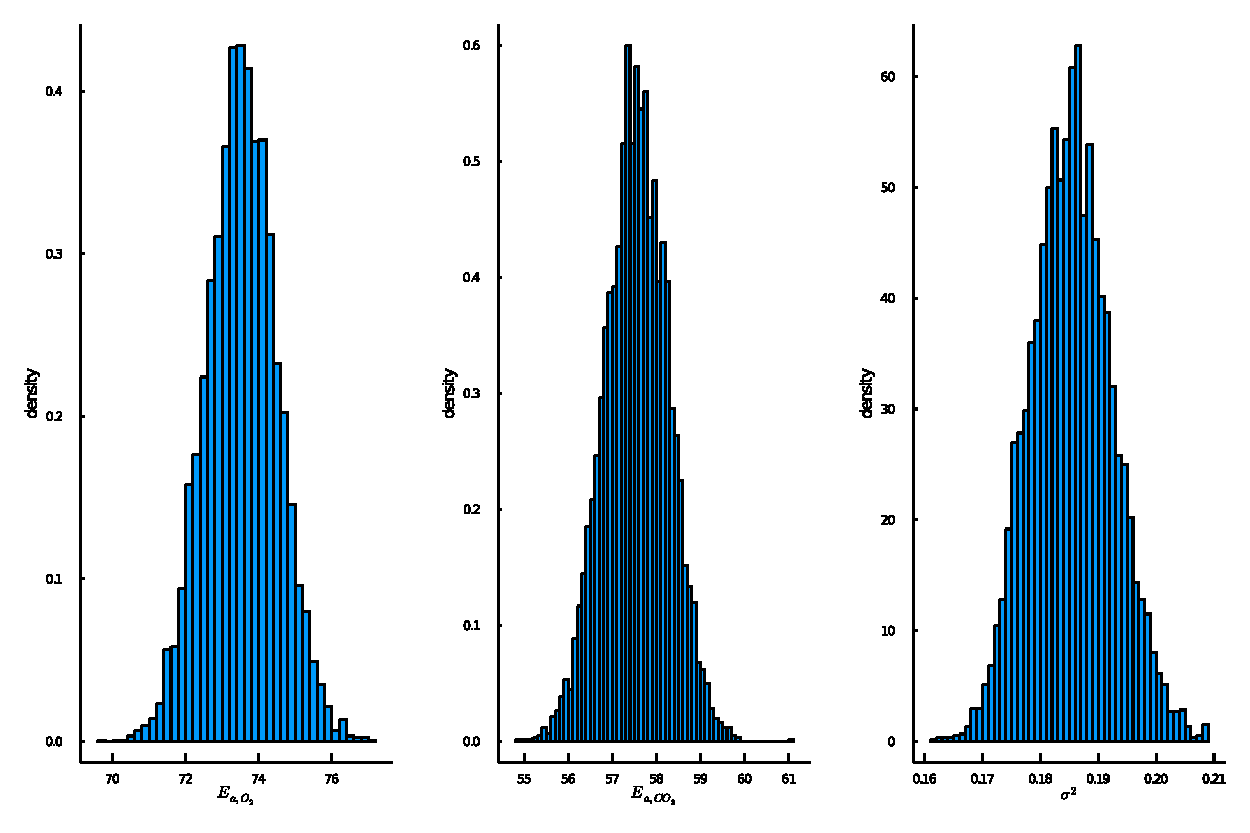
\includegraphics[width=0.99\textwidth]{figure/paper 2/test2.pdf}
	\caption{Summary of the Bayesian data analysis of the data in \textcite{ho} for the parameters of interest. {\color{red}This figure is stretched over two pages. The diagonal contains histograms of the Markov chain values of the six model parameters of interest. The orange dots denote the means. Above the diagonal, two-dimensional heatmaps are shown, visualizing the correlation between the Markov chain values for pairs of model parameters. Similarly, below the diagonal, scatter plots for $100$ Markov chain points are shown.}}
	\label{figprior}
\end{figure}
The estimation of the respiration inhibition parameter, $K_{\text{mn},\text{CO}_2}$, from the available data was problematic. For this reason, we had to reparametrize the model using the inverse of $K_{\text{mn},\text{CO}_2}$. As can be seen in the third histogram in Figure \ref{figprior}. $K_{\text{mn},\text{CO}_2}^{-1}$ takes values close to zero, which means $K_{\text{mn},\text{CO}_2}$ tends to infinity. The lack of information about $K_{\text{mn},\text{CO}_2}^{-1}$ can be explained as follows: to precisely estimate this parameter, both high $\oxy$ and $\coxy$ concentrations are needed. A high $\oxy$ concentration is required because otherwise there is no respiration that can be inhibited, and a high $\coxy$ concentration is required because otherwise the inhibition has a negligible effect. Data points in which both gasses posses a high concentration do not occur in the data of \textcite{ho}. {\color{red}The issues with the uncertainty about $K_{\text{mn},\text{CO}_2}$ were the catalyst for the development of our robust experimental design method. We found no other reliable way to quantify the uncertainty on this parameter, except working with a Markov chain.}
$K_{\text{m,f},\oxy}$ is the second hardest parameter to identify, from the data of \textcite{ho}, because the $\oxy$ concentration needs to be in a specific range for this parameter to have an effect on the outputs. An $\oxy$ concentration much higher than $K_{\text{m,f},\oxy}$ means no fermentation is happening at all, and an $\oxy$ concentration much lower than $K_{\text{m,f},\oxy}$ implies maximal fermentation. The third most difficult parameter to identify is  $K_{\text{m},\text{O}_2}$, because the model is only sensitive to this parameter when $\oxy$ concentrations are close to the value of this parameter.
\begin{figure}[H]
	\centering
	\begin{subfigure}[b]{0.3\textwidth}
		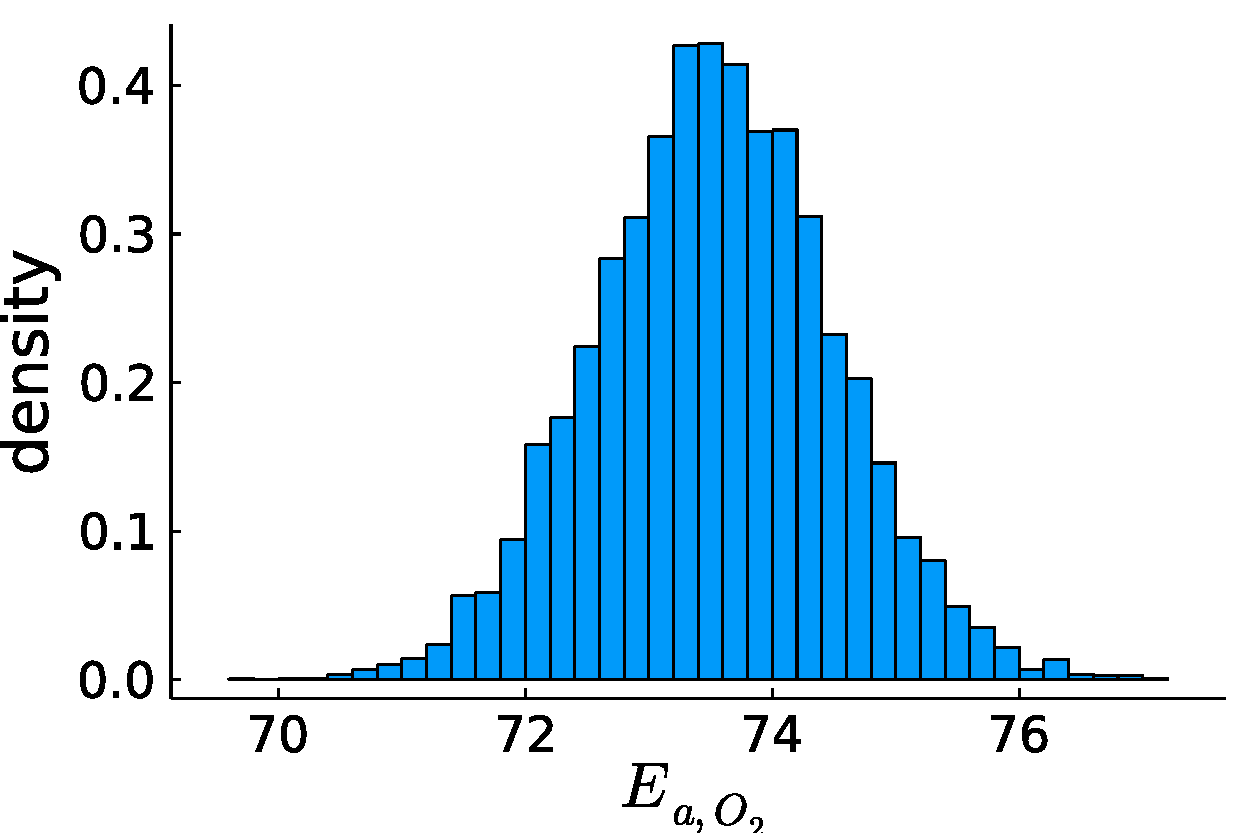
\includegraphics[width=1.0\textwidth]{figure/paper 2/nuisance1.pdf}
	\end{subfigure}
	\begin{subfigure}[b]{0.3\textwidth}
		\centering
		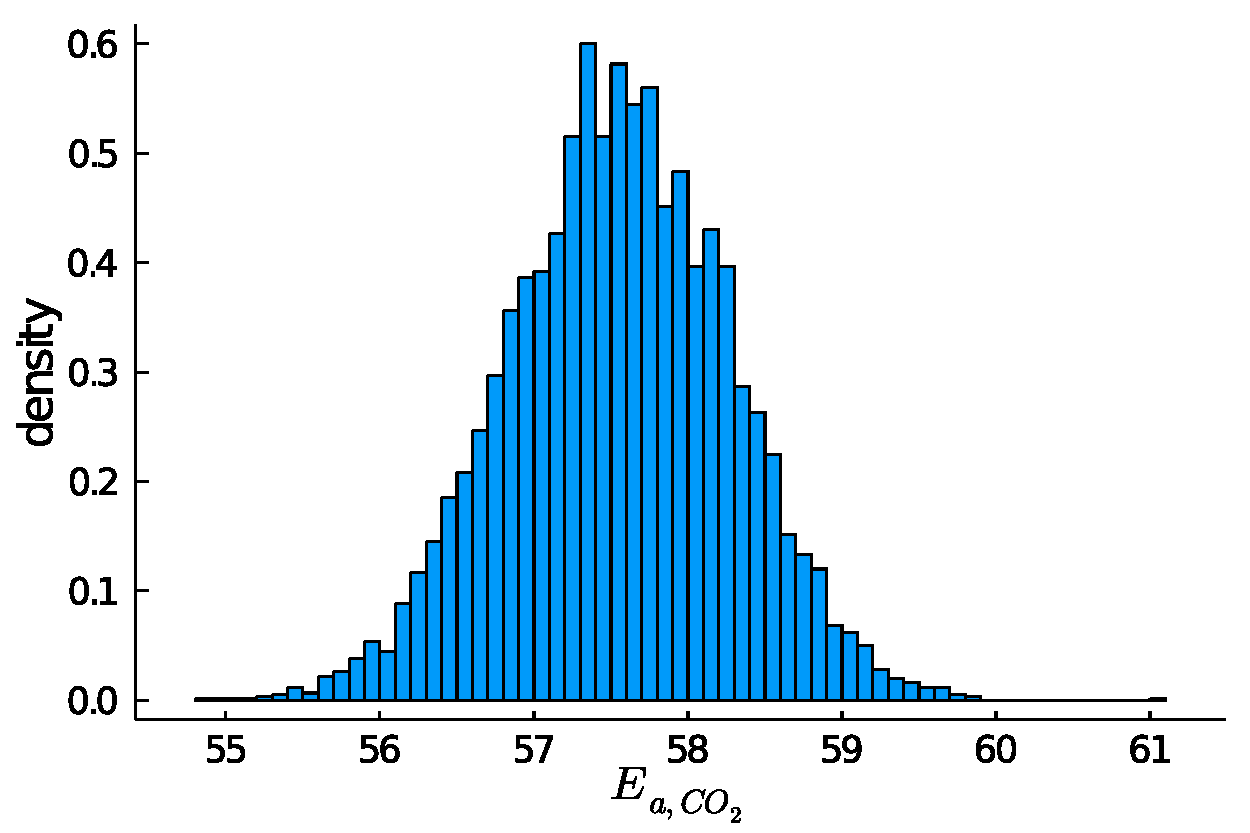
\includegraphics[width=1.0\textwidth]{figure/paper 2/nuisance2.pdf}
	\end{subfigure}
	\begin{subfigure}[b]{0.3\textwidth}
		\centering
		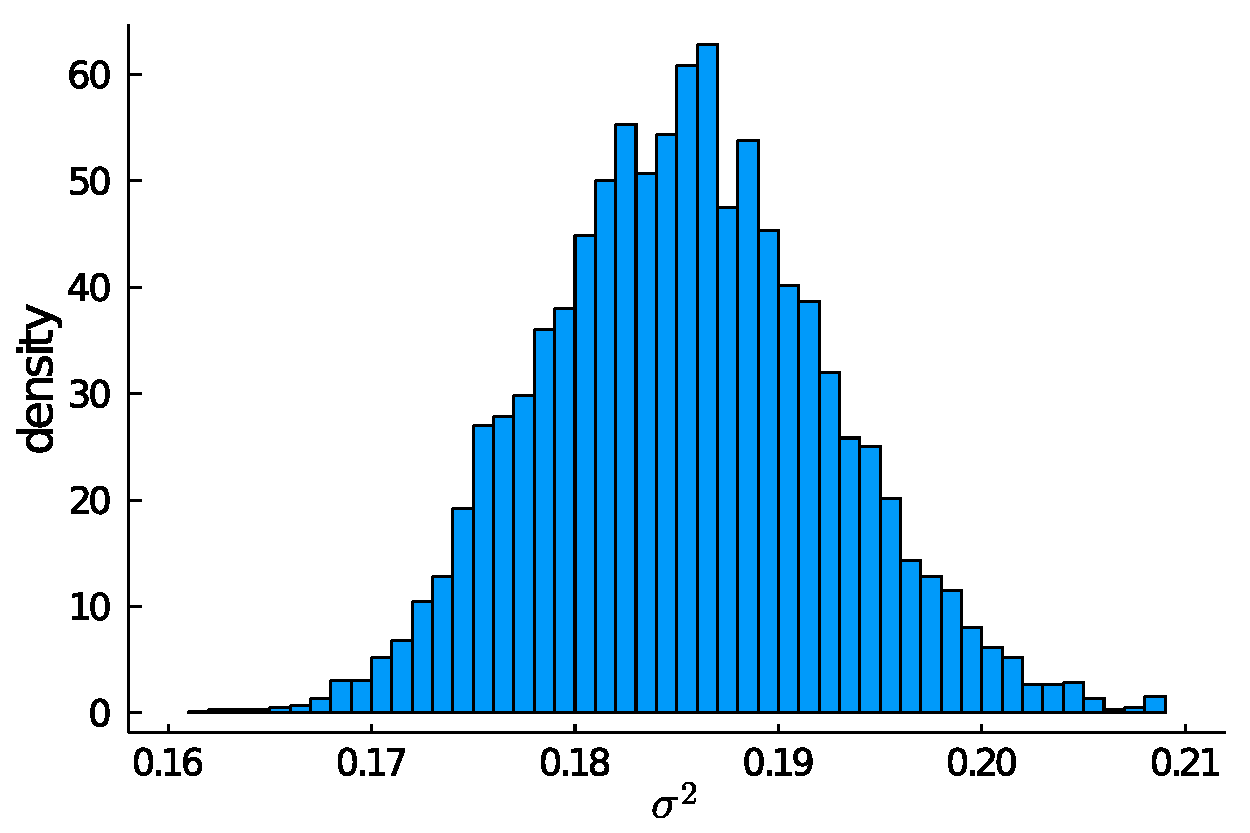
\includegraphics[width=1.0\textwidth]{figure/paper 2/nuisance3.pdf}
	\end{subfigure}
	\caption{Summary of our Markov-chain Monte-Carlo analysis of the data in \textcite{ho} for the nuisance parameters $E_{a,\oxy}$, $E_{a,\coxy}$ and $\sigma^2$.}
	\label{fignuisance}
\end{figure}
\subsection{Markov chain Details}
\label{sec_markov}
The data analysis was performed using the No U-Turn Sampling Markov-chain Monte-Carlo algorithm \parencite{hoffman}, as implemented in Turing.jl \parencite{ge}. We ran 4 parallel Markov chains each starting from the maximum likelihood estimates of the parameters, and each chain comprises 1500 steps. We utilized a flat prior in the physically possible regions of the unknown parameters. For all parameters this means that only positive values are possible, with $r_q$ being at most $1$.
\\
\\
We used the posterior distribution resulting from this Bayesian analysis of the experiments in \textcite{ho} as a prior distribution for the generation of the robust designs in this chapter. However, as calculating Bayesian optimal designs with the entire Markov chain is numerically quite intensive, we discarded the first 500 step, and thinned the remaining 1000 by a factor 40. This gave us 100 samples to calculate the Bayesian D-optimality criterion in Equation (\ref{pseudoD}). These are also the 100 values shown in the top right half of Figure \ref{figprior}.
\section{Results}
\label{sec_experiments}
In our examples, we consider experiments lasting $24$ h with measurements taken every $5$ minutes, i.e. $t_e = 24$ h and $N=288$. The maximum and minimum flow rates are equal to $1\text{ l h}^{-1}$ and $0.1\text{ l h}^{-1}$, respectively. The input gas concentrations are allowed to vary between $0 \text{ kPa}$ and $21\text{ kPa}$. We did not use a minimum flow rate of $0\text{ l h}^{-1}$, because at zero flow there is no difference in system response between a maximal or minimal gas input concentration. This implies that the design selection criteria from Equations (\ref{localD}) and (\ref{pseudoDcalc}) are flat in certain directions, causing numerical issues for gradient based optimizers. Working with a strictly positive minimum flow rate avoids this issue. {\color{red}Another reason to use strictly positive flows is to ensure that there is an outflow that can be measured.}
\subsection{Locally Optimal Designs for the Respiration and Fermentation Model}
We take the average values of the Markov chains of the parameters of interest, as well as the average of the Markov chain values of the {\color{red}measurement variance} $\sigma^2$ to evaluate the local D-criterion in Equation (\ref{pseudoD}). These values are shown in Table \ref{tableLocal}, and indicated by a bullet in the histograms on the diagonal of Figure \ref{figprior}. We start by analyzing the effect of an increasing refinement of the discretization of the inputs $\bm u(t)$. In Figure \ref{figconvergence}, which shows the local D-criterion value as a function of the number of times the input signal is allowed to switch, we see that the D-criterion no longer improves noticeably after $M = 48$, which corresponds to a switch every half hour. The experimental design obtained with $M = 12$, which corresponds to a switch every two hours, already performs well. Therefore, in the remainder of this chapter, we consider $\oxy$, $\coxy$ and flow rate inputs that remain constant for two-hour time periods.
\begin{table}[h!]
	\centering
	\setlength{\tabcolsep}{4pt} 
	\small
	\begin{tabular}{|c c c c c c c|}

		\hline
		$V_{\text{m},\oxy}$ & $K_{\text{m},\oxy}$ &  $K_{\text{mn},\text{CO}_2}$ & $r_q$ & $V_{\text{m,f,}\coxy}$ & $K_{\text{m,f},\oxy}$ & $\sigma^2$\\ [0.5ex] 
		\hline
		$\mu$mol$\text{ kg}^{-1}$ $\text{ s}^{-1}$ & kPa & kPa & - & $\mu$mol$\text{ kg}^{-1}$ $\text{ s}^{-1}$& kPa & $\text{mol}^2$$\text{ m}^{-6}$	\\ [0.5ex] 
		\hline
		0.320 & 5.61 & 484.4 & 0.655 & 0.121 & 0.224 & 0.186\\ [1ex] 
		\hline
	\end{tabular}
	\caption{Parameters used for the optimization of the construction of the locally optimal designs.}
	\label{tableLocal} 
\end{table}
\begin{figure}[h]
	\centering
	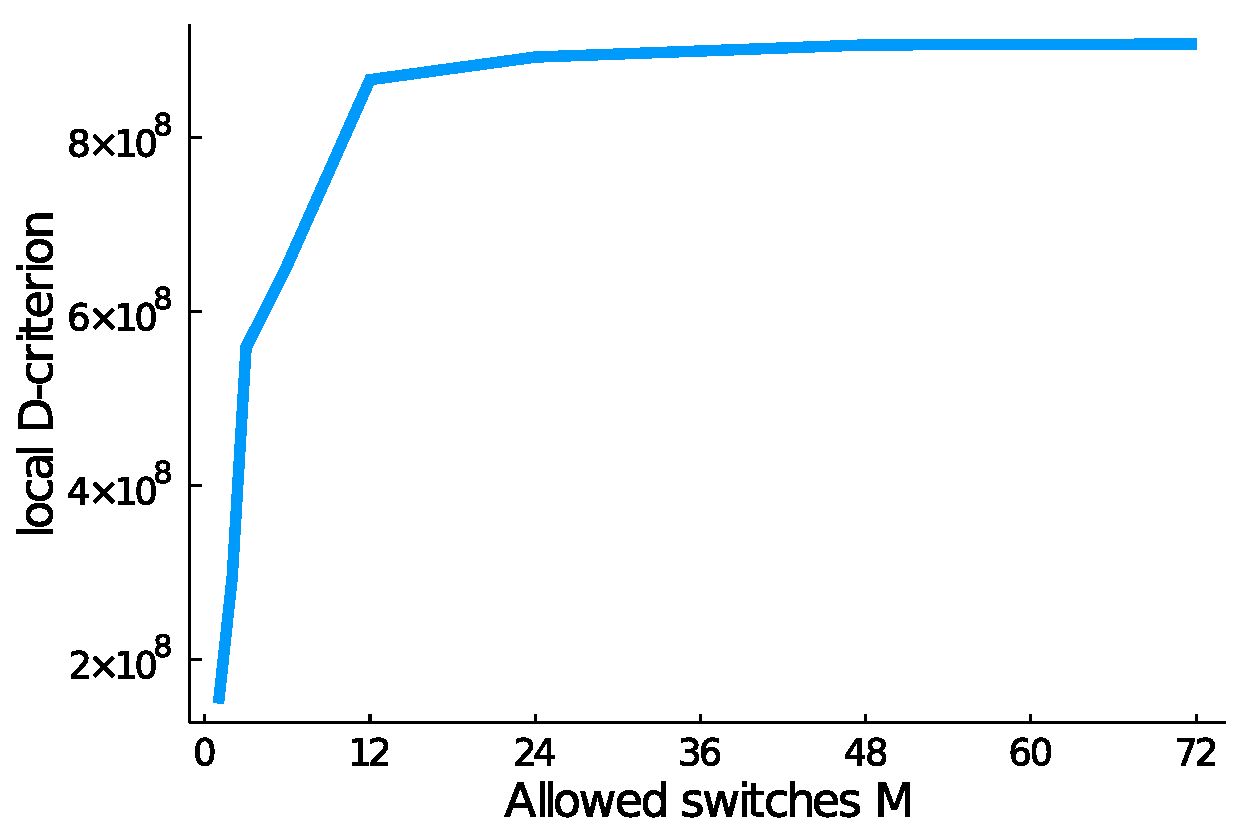
\includegraphics[width=0.9\textwidth]{figure/paper 2/convergence.pdf}
	\caption{Convergence of the local D-optimality criterion for finer discretizations of the controls.}
	\label{figconvergence}
\end{figure}
The locally optimal design for the scenario in which the inputs are allowed to vary every two hours is shown in more detail in Figures \ref{figlocala} and  \ref{figlocalb}, together with the simulated outputs in Figure \ref{figlocalc}, evaluated at the values of the model parameters used to optimize the design. {\color{red}The gas concentrations are converted to pressures to aid interpretation.} During the interval from $2$ h to $4$ h, both $\oxy$ and $\coxy$ are pumped into the jar, which causes high concentrations of the two gasses to be present at the same time. We noted before that, due to the lack of such conditions in \textcite{ho}, it was impossible to estimate $K_{\text{mn},\text{CO}_2}$ well from their data. However, the $\oxy$ concentration cannot remain high throughout the entire experiment, as then there would be insufficient information about non-saturated respiration, i.e. to estimate $K_{\text{m}, \oxy}$ precisely. The $\oxy$ concentration must decrease further to levels at which fermentation starts to occur for $K_{\text{m,f},\oxy}$ to become estimable. This explains why air, with zero $\oxy$ inlet concentrations is pumped into the jar in the interval between $10$ h and $12$ h. The $\coxy$ inlet concentration is also zero during that time interval due to the fact that the $\coxy$ concentration is not allowed to run up too high, as this compromises the ability to precisely determine the fermentation parameters. This can be intuitively understood by considering the system in an extreme scenario where the atmosphere in the jar consists entirely of $\coxy$. In this scenario, the outflow will also be pure $\coxy$ regardless of the values of the fermentation parameters. Information about the fermentation parameters is then only incorporated in the outflow rate, but this is not a measured output. This illustrates how optimal experiments automatically take into account the specifics of the measurement setup.  The pumping action at $18$ h, again involving zero $\oxy$ and $\coxy$ concentrations, is performed for similar reasons.
\begin{figure}[t]
	\centering
	\begin{subfigure}[b]{0.45\textwidth}
		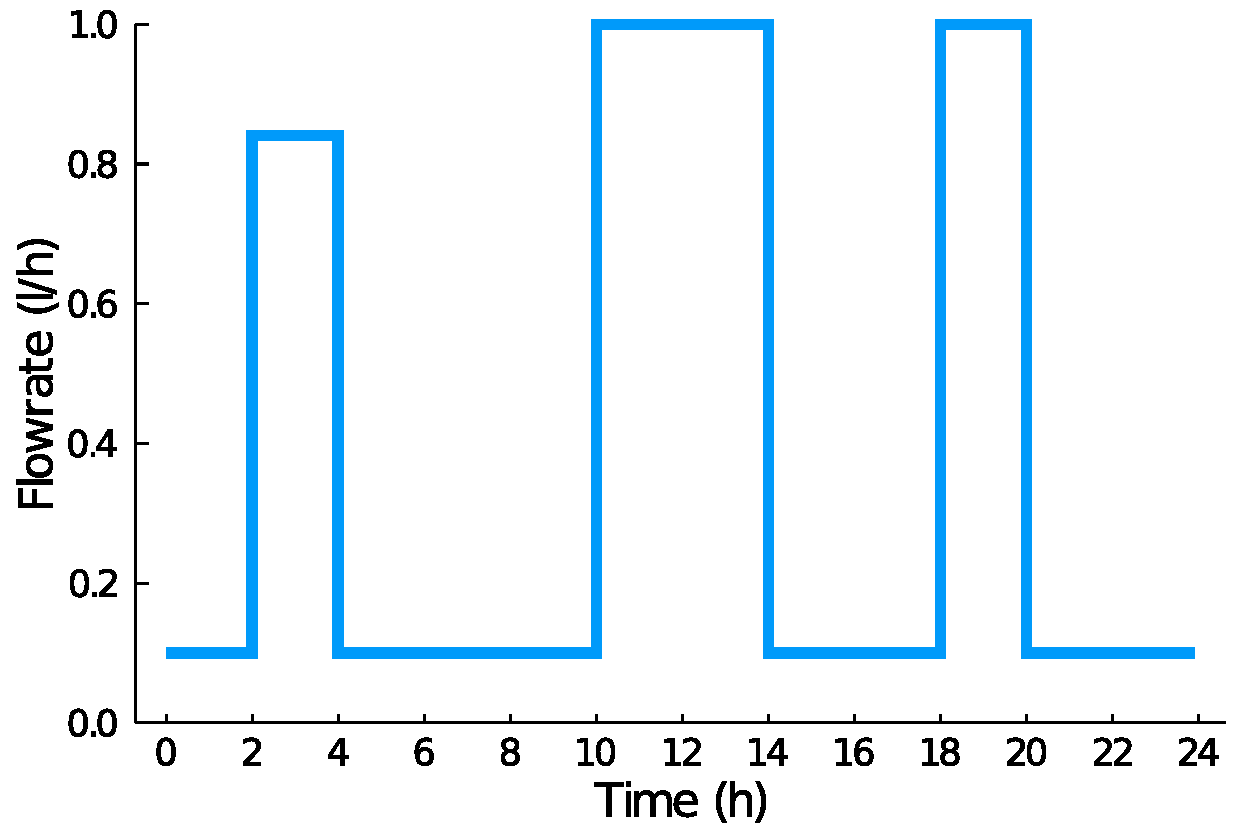
\includegraphics[width=1.0\textwidth]{figure/paper 2/l12_input_flow.pdf}
		\caption{Input flow.}
		\label{figlocala}
	\end{subfigure}
	\begin{subfigure}[b]{0.45\textwidth}
		\centering
		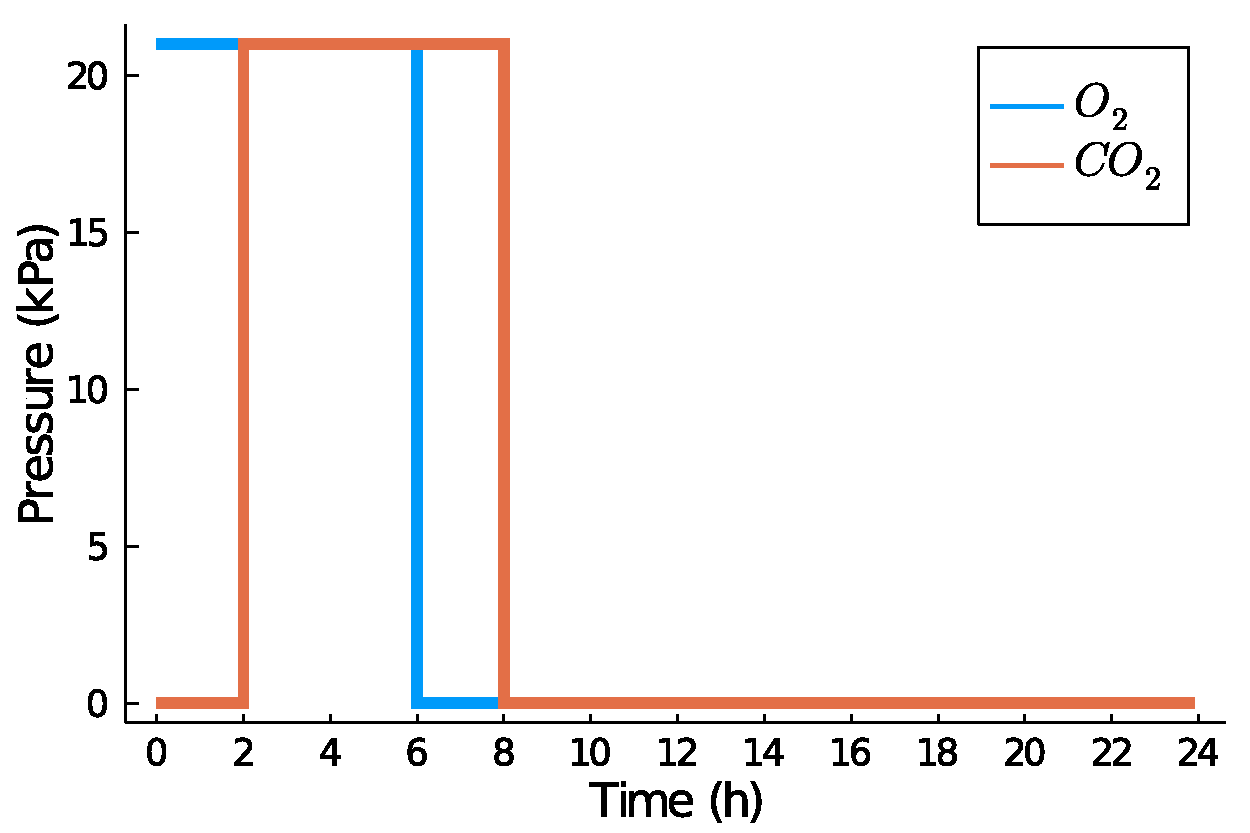
\includegraphics[width=1.0\textwidth]{figure/paper 2/l12_input_gass.pdf}
		\caption{Input gasses.}
		\label{figlocalb}
	\end{subfigure}
	\\
	\begin{subfigure}{0.45\textwidth}
		\centering
		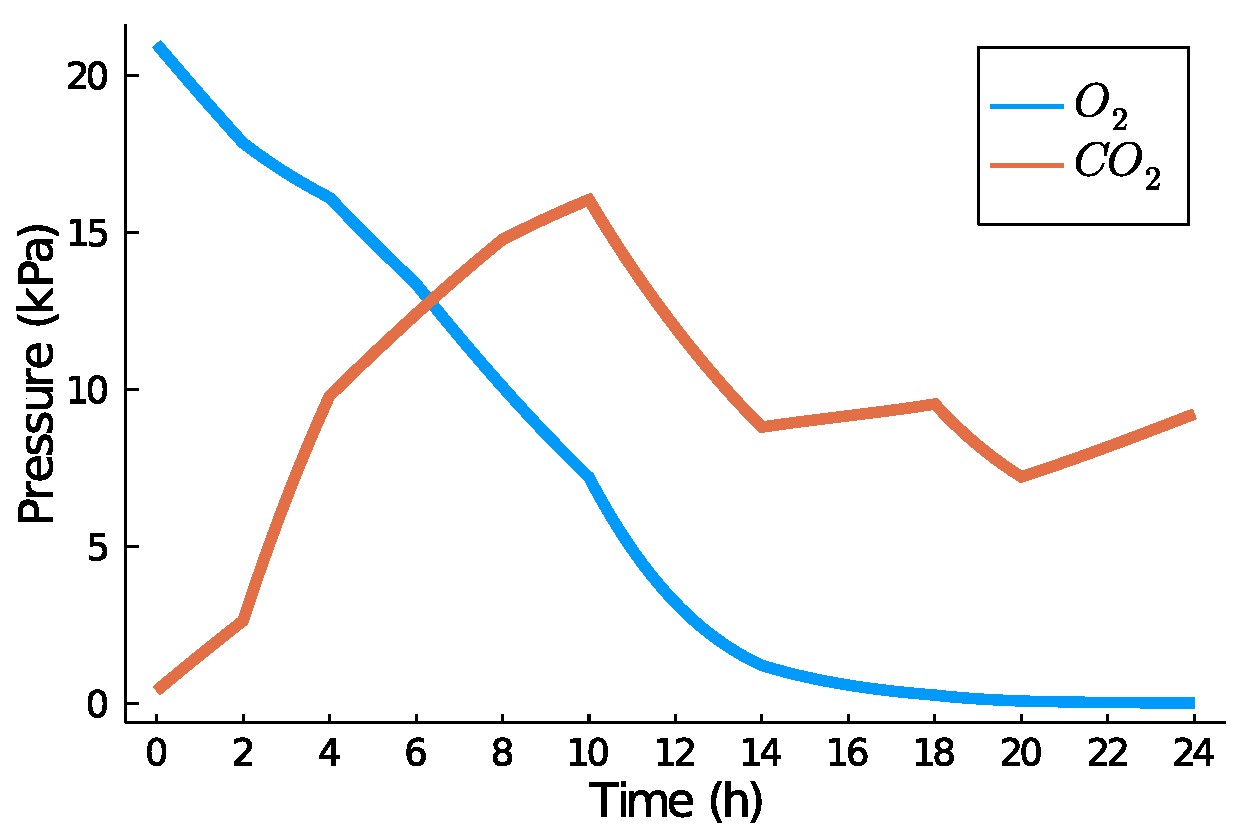
\includegraphics[width=1.0\textwidth]{figure/paper 2/l12_output.pdf}
		\caption{Output gasses.}
		\label{figlocalc}
	\end{subfigure}
	\caption{Locally optimal experiment and simulated output, with control input switches every two hours.}
	\label{figlocal}
\end{figure}
Figure \ref{figlocald} shows the coefficients of variation of all six model parameters, {\color{red}defined as the ratio of the standard errors, as given by the diagonal elements of the inverse of the FIM, and the model parameter values used for the generation of the local optimal design}. The three inhibition parameters ($K_{\text{m},\oxy}$, $K_{\text{mn},\text{CO}_2}$ and $K_{\text{m,f},\oxy}$) remain the most difficult {\color{red}ones} to estimate. Now, however, in our experiment involving a single jar, instead of using the data from $50$ jars, made available to us by \textcite{ho}, the model parameters can be estimated much more precisely.
\begin{figure}[h]
	\begin{subfigure}[b]{0.45\textwidth}
		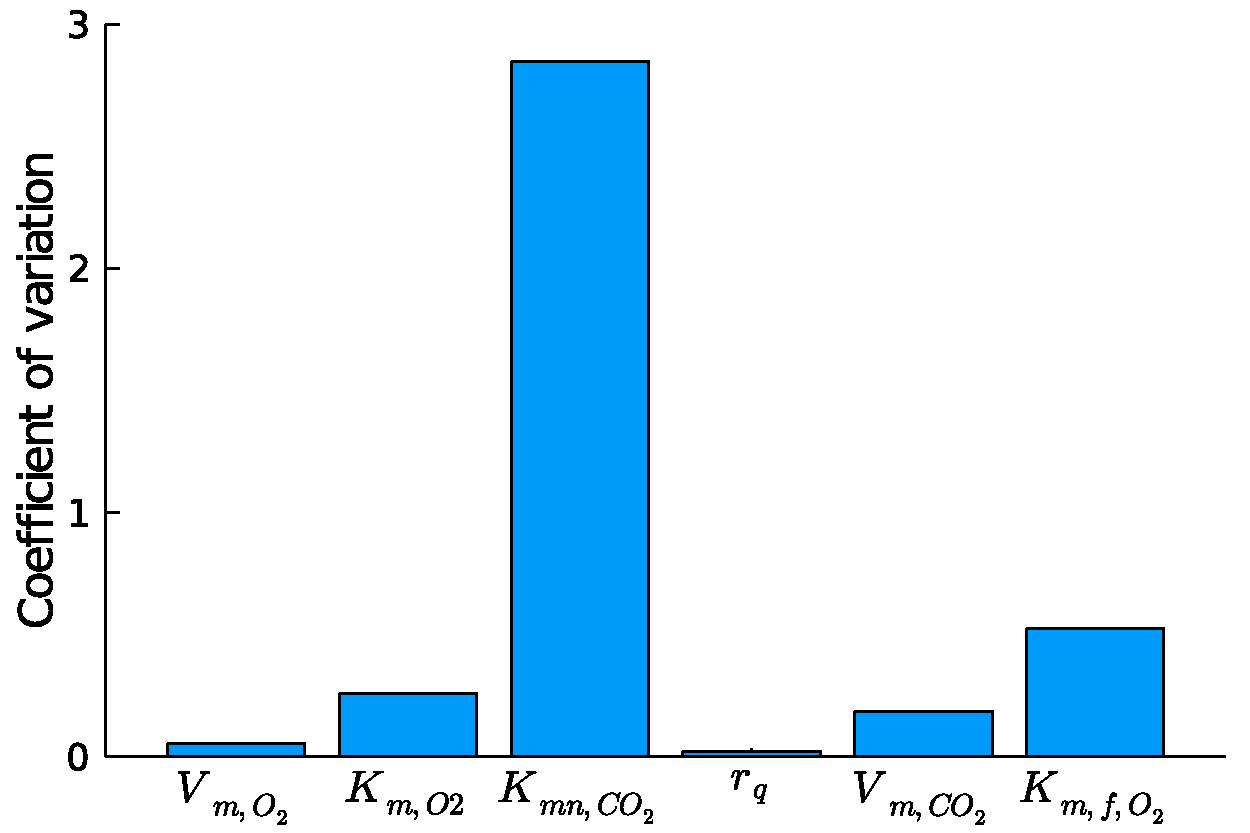
\includegraphics[width=1.0\textwidth]{figure/paper 2/l12_var.pdf}
		\caption{coefficients of variation}
		\label{figlocald}
	\end{subfigure}
	\begin{subfigure}[b]{0.45\textwidth}
		\centering
		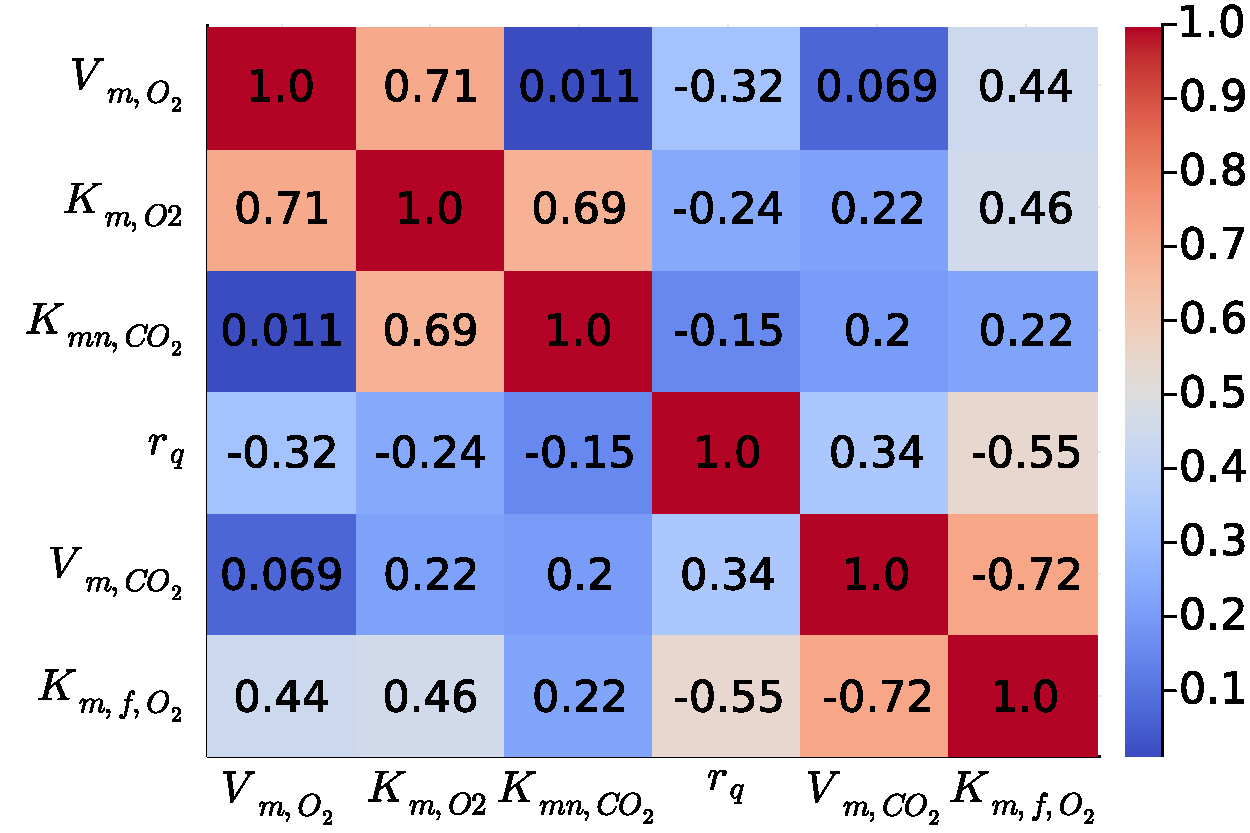
\includegraphics[width=1.0\textwidth]{figure/paper 2/l12_corr.pdf}
		\caption{absolute value of correlations}
		\label{figlocale}
	\end{subfigure}
	\caption{Summary of the information gained from the locally optimal experiment in Figure \ref{figlocal}, {\color{red} with local D-criterion equal to $8.67 \e{8}$}.} 
\end{figure}
Figure $\ref{figlocale}$ shows a map of the absolute values of the correlations of the estimates that would be obtained if the locally optimal experiment were to be used. Because there are no strong correlations between the first three parameters and the last three parameters, we can thus visualize the FIM in Equation (\ref{FIM}) using two ellipsoids. {\color{red}The axes of the first ellipsoid are in the directions of the eigenvectors of the inverse of the top left quarter (a 3 by 3 matrix) of the FIM, and the lengths of the axes are the corresponding eigenvalues. The second ellipsoid is similarly based on the bottom right quarter.} These ellipsoids are shown in Figures \ref{figlocalf} and \ref{figlocalg} for the experiment allowing changes in inputs every two hours, {\color{red}and are compared to the ellipsoids in blue resulting from the heuristic experimentation technique used by \textcite{ho} with the volume of the jar, mass of pears, initial conditions, sampling times and total experimentation time equalized between the two methods. The volume of the ellipsoids of the locally optimal experiment are smaller.}
\begin{figure}[H]
	\begin{subfigure}[b]{0.45\textwidth}
		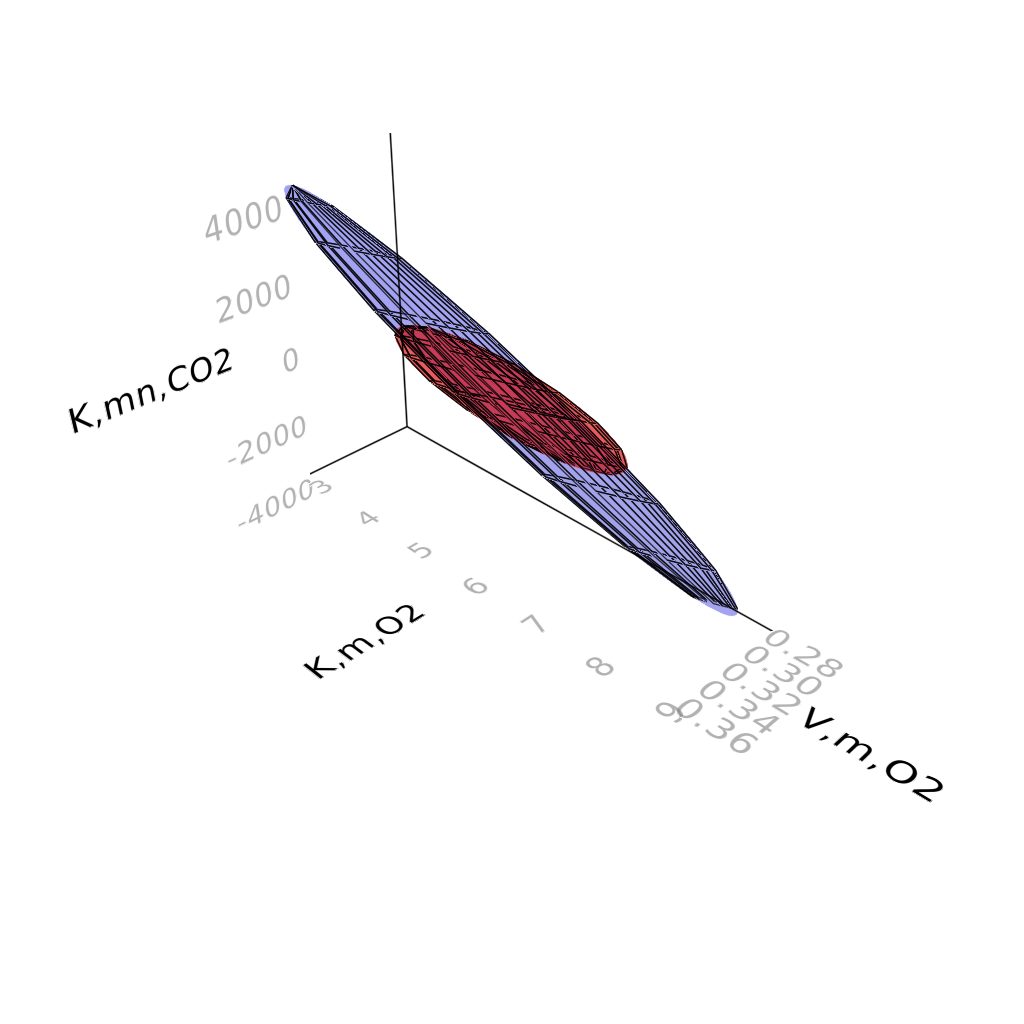
\includegraphics[width=1.0\textwidth]{figure/paper 2/ellipsoid1_3.png}
		\caption{first three parameters \\ $\qquad(V_{\text{m},\oxy}$, $K_{\text{m},\oxy}$, $K_{\text{mn},\text{CO}_2)}$.}
		\label{figlocalf}
	\end{subfigure}
	\begin{subfigure}[b]{0.45\textwidth}
		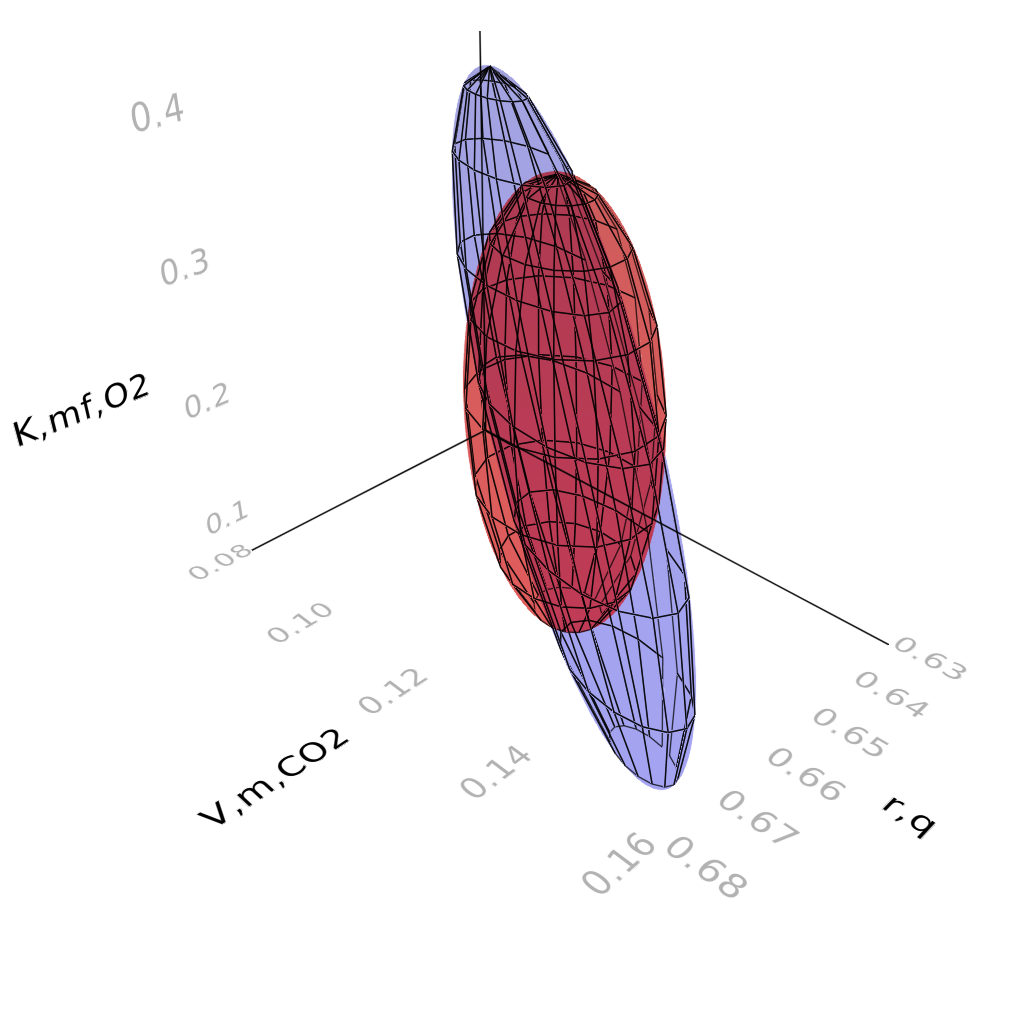
\includegraphics[width=1.0\textwidth]{figure/paper 2/ellipsoid4_6.png}
		\caption{last three parameters \\ $\qquad (r_q$, $V_{\text{m,f,}}$, $K_{\text{m,f},\oxy)}$.}
		\label{figlocalg}
	\end{subfigure}
	\caption{95\% confidence ellipsoids comparing {\color{red}the locally optimal experimental design (red) and the heuristic experimental design technique from \textcite{ho} (blue)}.} 
	\label{figellipsoid}	
\end{figure}
\subsection{Bayesian Optimal Designs for the Respiration and Fermentation Model}
We now continue by searching a more robust design than the locally optimal design in Figure \ref{figlocal}. Instead of optimizing the determinant of the FIM in Equation (\ref{FIM}) for the means of the Markov chain values, we optimize the mean determinant for a thinned version of the Markov chain. These values are graphically shown by the blue bullets in the lower left hand part of Figure \ref{figprior}, {\color{red}these values can also be found in Appendix \ref{appendix}}. The design found by maximizing the robust optimality criterion in Equation (\ref{pseudoDcalc}) is shown in Figures \ref{figbayesiana} and \ref{figbayesianb}. The simulated output for all values of the thinned Markov chain is shown in Figure \ref{figbayesianc}. The robust design exhibits several similarities to the locally optimal design, but also some key differences. The occurrence of a pumping action in the time interval between $2$ h and $4$ h as well as the interval between $10$ h and $14$ h is similar to that in the locally optimal design in Figure \ref{figlocala}. Furthermore, there are no differences in $\oxy$ and $\coxy$ input concentrations between the robust and locally optimal design. One main difference between the robust experimental design and the locally optimal one is that, in the former, the first pumping action is less intense, i.e. the flow rate only amounts to $0.5$ l$\text{h}^{-1}$, as opposed to  $0.8$ l$\text{h}^{-1}$, in the locally optimal design. A second main difference is the absence of the third pumping action in the robust design. We hypothesize this is because  less pumping actions must occur to ensure a high $\coxy$ concentration when inhibition of respiration by $\coxy$ only happens at high $\coxy$ concentrations, which is possible, since we have little prior knowledge about $K_{\text{mn},\text{CO}_2}$.
\begin{figure}[H]
	\centering
	\begin{subfigure}[b]{0.45\textwidth}
		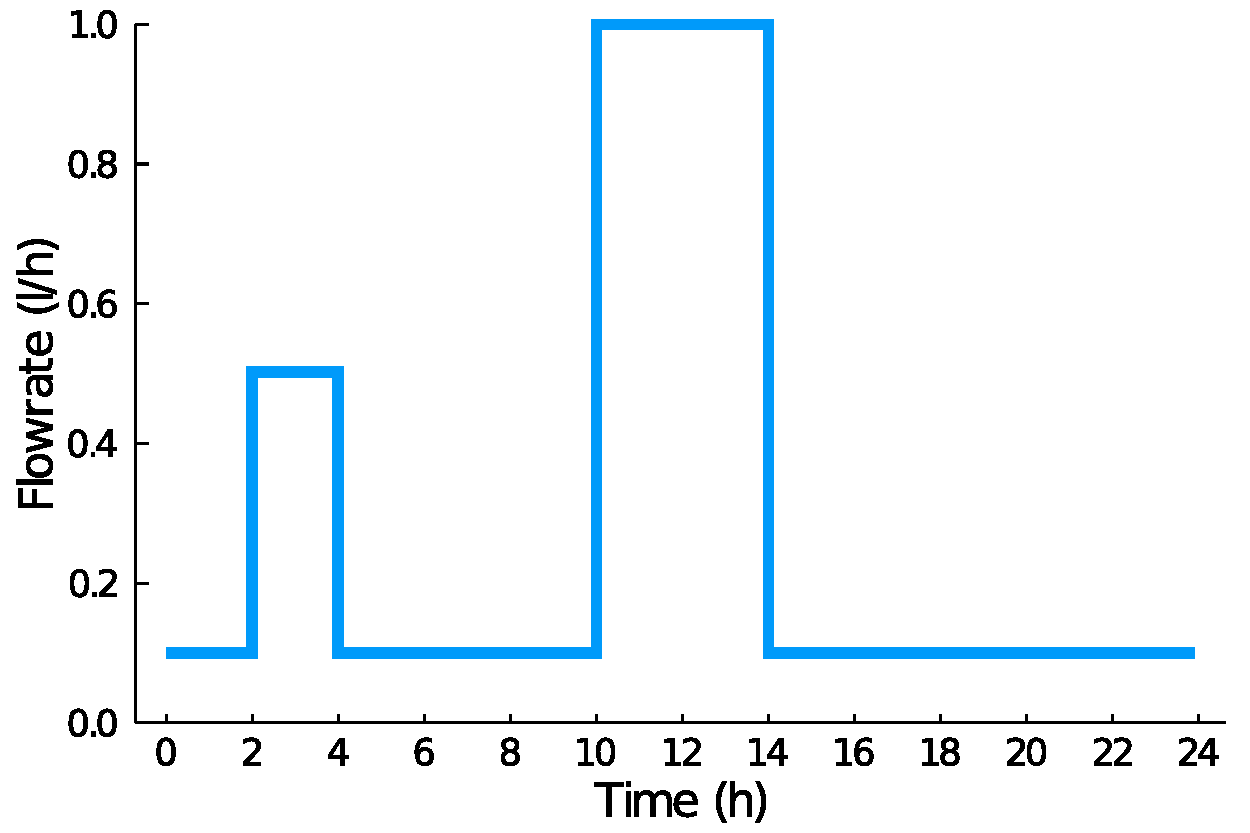
\includegraphics[width=1.0\textwidth]{figure/paper 2/b12_input_flow.pdf}
		\caption{Input flow.}
		\label{figbayesiana}
	\end{subfigure}
	\begin{subfigure}[b]{0.45\textwidth}
		\centering
		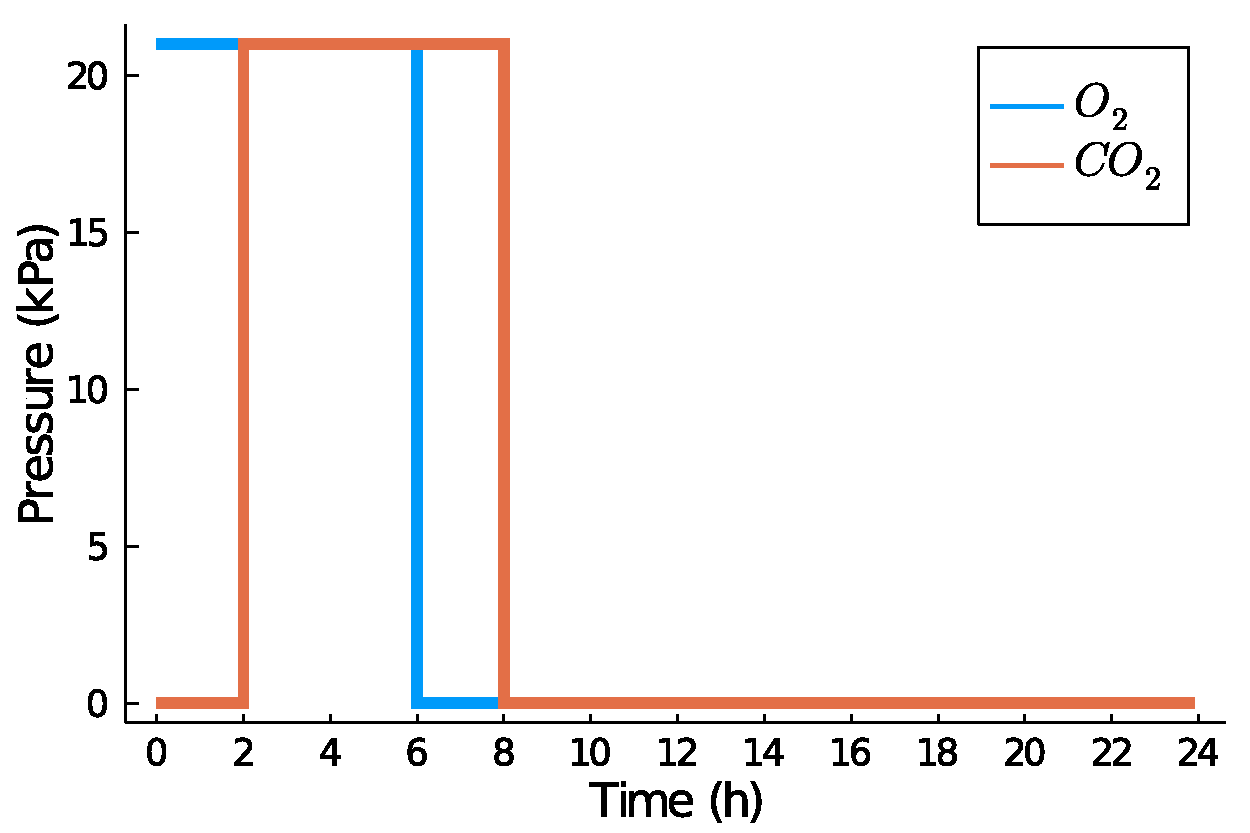
\includegraphics[width=1.0\textwidth]{figure/paper 2/b12_input_gass.pdf}
		\caption{Input gasses.}
		\label{figbayesianb}
	\end{subfigure}
	\\
	\begin{subfigure}{0.45\textwidth}
		\centering
		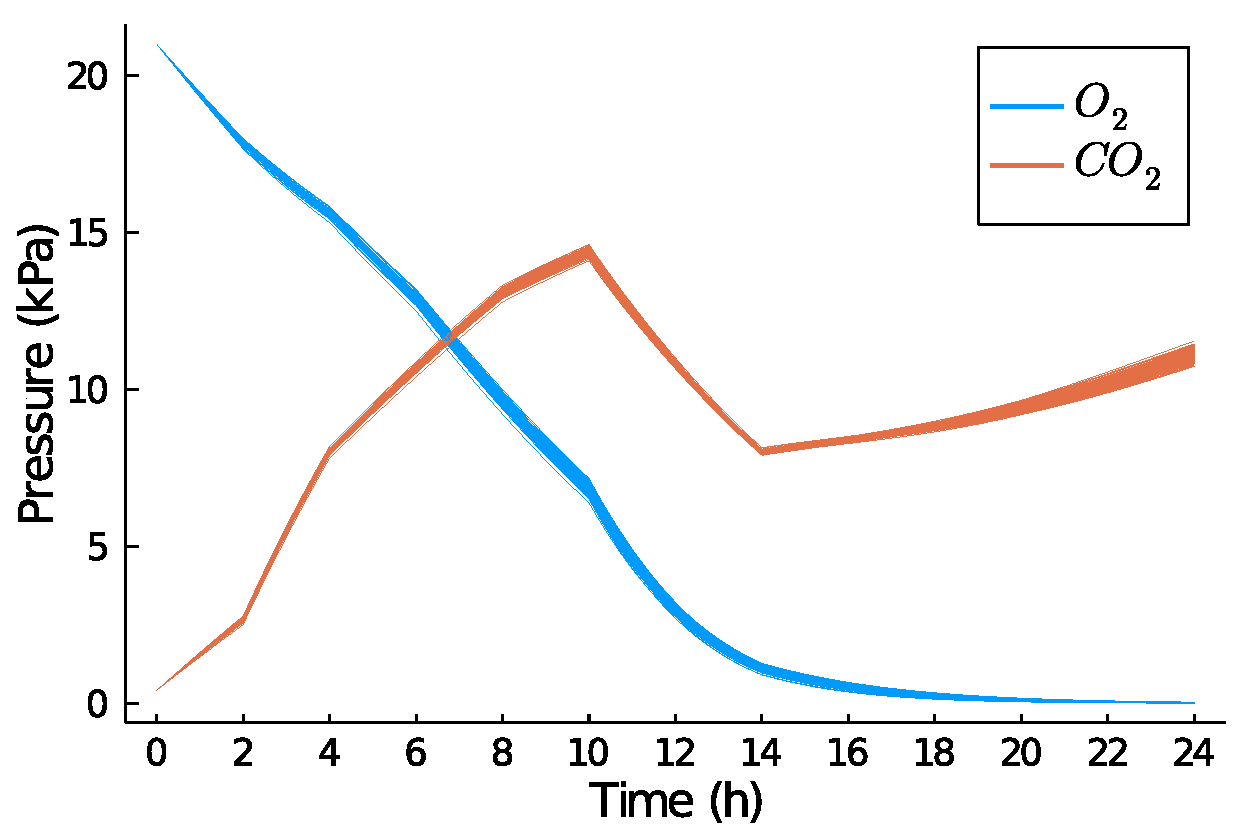
\includegraphics[width=1.2\textwidth]{figure/paper 2/b12_output.pdf}
		\caption{Output, evaluated at each of the model parameter values from the thinned Markov chain.}
		\label{figbayesianc}
	\end{subfigure}
	\caption{Robust optimal experiment and simulated output, obtained using $100$ parameter values from the Markov chain and control input switching every two hours.}
	\label{figbayesian}
\end{figure}
Figure \ref{figbayesianhistogram} shows the difference in performance between the robust and the locally optimal experiment. More specifically, the histogram shows the difference between the determinant of the FIM in Equation (\ref{FIM}) for both the robust and locally optimal design at all $6000$ model parameter values from the Markov chain. For many possible model parameter values, the locally optimal and robust design perform almost equally well. However, the histogram clearly has a heavy right tail, showing that, for some parameter values, the Bayesian design performs significantly better. As the histogram does not posses a heavy left tail, the reverse is not true. The robust design is thus substantially less sensitive to the exact values of the model parameters. It therefore provides better guarantee for a highly informative experiment than the locally optimal design. Since this result holds for the entire Markov chain and not just the thinned version, we can be confident that the thinned version is sufficient to summarize the prior uncertainty, and that the resulting robust design only works well for the specific model parameter values used to evaluate the optimality criterion in Equation (\ref{pseudoDcalc}). Finally, the positive mean value for the difference in determinants, indicated by the orange dot in Figure \ref{figbayesianhistogram}, proves that Bayesian design is expected to do better for the region of prior uncertainty.
\begin{figure}[H]
	\centering
	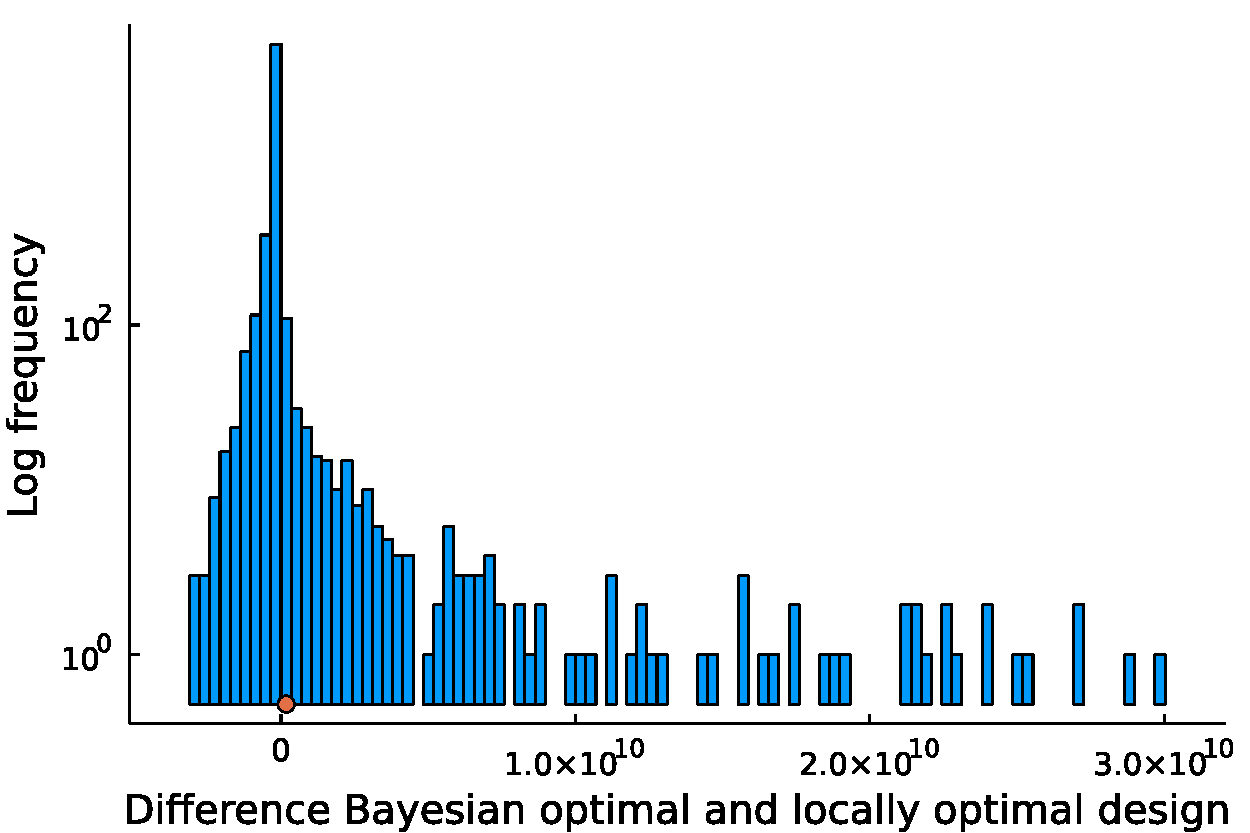
\includegraphics[width=0.9\textwidth]{figure/paper 2/histogram.pdf}
	\caption{Histogram of difference in determinants of the FIM of the robust and locally optimal designs for $6000$ parameters from the prior distribution. Positive values mean the robust design performs better.}
	\label{figbayesianhistogram}
\end{figure}
{\color{red}In Table \ref{tableRobust}, we also compare our robust experimental design method based on a Markov-chain Monte-Carlo chain, which can approximate arbitrary distributions, to the robust experimental design method of \textcite{telen}, which uses 13 sigma points to summarize the uncertainty on the model parameters, and is thus computationally less intensive. The latter results in a design that performs worse than the locally optimal design, showing that sigma points do not always provide good summary of the uncertainty in the model parameters.
	\begin{table}[h!]
		\color{red}
		\centering
		\begin{tabular}{||c c c c||}
			\hline
			&Markov-chain Monte-Carlo& locally & sigma point \\
			&optimal design& optimal design &optimal design \\
			\hline
			Robust & &  &  \\
			D-criterion & 1.26\e{10}&  1.22\e{10}& 9.83\e{9} \\
			\hline
		\end{tabular}
		\caption{Parameters used for the optimization of the construction of the locally optimal designs}
		\label{tableRobust} 
	\end{table}
}
\section{Discussion and Future Work}
\label{sec_discussion}
\subsection{Alternative Information Criteria}
In this chapter, we presented a robust experimental design methodology for dynamic models and applied that methodology to precisely estimate the respiration and fermentation parameters of {\color{red}pear fruit}. We achieved this by quantifying the information content of the experiments using the determinant of the Fisher information matrix averaged over a prior distribution, represented by a Markov-chain. {\color{red}However, the Fisher information matrix is only an approximation of the inverse of the model parameter covariance matrix. \textcite{schenkendorf} suggest another approach to approximate the covariance matrix based on simulating multiple possible data-sets, and estimating the model parameters from each data-set. This approach is numerically much more intensive than an approach based on the FIM, and is therefore infeasible in the context of optimal experimental design. Another promising} approach would be to quantify information based on the expected Kullback-Leibler divergence (KL-div) between the prior and posterior distributions \parencite{lindley}. For {\color{red}experiments with a large number of observations}, the expected KL-div is asymptotically equal to our {\color{red}robust} D-optimality criterion. For {\color{red}a small number of measurements}, the KL-div approach might be superior as it does not utilize normal approximations. One major downside of using the KL-div is its computational complexity, as it involves calculating a high dimensional integral over all possible outcomes $\bm y $ of the experiment. This is generally done using a double loop Monte-Carlo integration method \parencite{ryan}. Some research has been done using this method for determining optimal sampling times of dynamic systems \parencite{overstall2}, but this work does not consider optimal control. Therefore, the dynamic system in  \textcite{overstall2} does not need to be  solved repeatedly for different control actions. Instead, only a single dynamic system needs to be solved that can be evaluated at different possible sampling times. Selection of input profiles based on the KL-div is considered in \textcite{liepe}, but only for a small  discrete set of possible input profiles. In contrast, in our paper, we optimize the experimental design over a large continuous space of possible experimental designs. Recently, advances have been made in lowering the computational burden of the KL-div based approach by considering {\color{red} surrogate functions that approximate the KL-div based on polynomial chaos expansions \parencite{paulson}. Another approach to lower the computational burden is based on} variational Bayesian techniques \parencite{foster}, where the inner Monte Carlo loop is replaced by optimizing a variational distribution. This technique then allows for jointly optimizing the design and variational parameters \parencite{foster2}. In future work, we will employ these variational Bayesian techniques for adaptive dynamic experiments, where the design is modified online as data is collected.
\subsection{State Discretization}
In this chapter, we discretized only the controls $\bm u$, but not the states $\bm x$. The discretization of states is applied using multiple shooting and collocation based dynamic optimization approaches \parencite{biegler}. Generally, these methods lead to optimization problems that are faster to solve, as they do not require repeatedly solving differential equals, but which might lead {\color{red}to less accurate results. The is because we found that solving the dynamic system with model parameters values equal to those of the heavy right tail in Figure \ref{figbayesianhistogram} requires many more steps than the other parameter values form the Markov chain. Thus unless the discretization is chosen fine enough, the approximation for the troublesome parameters in the tail might not suffice.}  Besides the faster computing time, one additional reason to consider discretization of the states would be the presence of additional constraints on the states. This is because violations of such constraints are difficult to check without a discretization. Our optimization problem did not involve any such additional state constraints. \textcite{nimmegeers} provide a more detailed discussion on the incorporation of constraints into optimal dynamic experiments.
\subsection{Reverse Automatic Differentiation}
We used forward mode automatic differentiation to calculate the sensitivities to the unknown parameters $\bm \theta$, required to obtain the FIM in Equation (\ref{FIM}), and this was further nested to calculate the gradient of the D-criteria in Equations (\ref{localD}) and (\ref{pseudoDcalc}) with respect to the control parameters $\bm u$. Forward mode automatic differentiation generally performs well for functions with a small number of inputs, relative to the number of outputs. For our respiration model, it thus was a good choice for calculating the unknown parameter sensitivities present in the FIM. Reverse mode automatic differentiation performs better for functions with many more outputs than inputs. It thus seems like a natural choice to calculate the gradients necessary for the optimization of the control parameters. However, there is currently not yet a mature implementation of reverse over forward mode automatic differentiation in the Julia ecosystem \parencite{rackauckas2}.
\section{Conclusion}
This chapter presented a pioneering study about the usefulness of robust optimal dynamic experiments for non-linear modeling in postharvest research. Robust designs work well for a range of possible model parameter values. Robust design methods require the specification of a prior distribution for the model parameters. Current methods in the literature only work for parametric prior distributions. The available prior information about respiration and fermentation of pear fruit could not be adequately summarized using a parametric distribution, thus we developed a novel experimental design methodology based on a Markov-chain Monte-Carlo analysis of a prior data-set. This Markov chain can approximate arbitrary distributions. We used this methodology to construct robust D-optimal dynamic experimental designs for the estimation of the Michaelis-Menten respiration and fermentation parameters of Conference pear. These robust designs perform better than locally D-optimal designs, which are optimized using a single initial guess for the model parameters, {\color{red}and also outperform other robust methods}.
\chapter{Adaptive and Robust Experimental Design for Linear Dynamic Models using the Kalman Filter}
\label{paper3}
This chapter has been written by Arno Strouwen with feedback from Professors Goos and Nicolaï.
\\
\\
{\color{red}Source code available upon request.}
\section*{Abstract}
Current experimental design techniques for dynamic systems often only incorporate measurement noise, {\color{red}while} dynamic systems also involve process noise. To construct experimental designs we need to quantify their information content. The Fisher information matrix is a popular tool to do so. Calculating the Fisher information matrix for linear dynamic systems with both process and measurement noise involves estimating the uncertain dynamic states using a Kalman filter. The Fisher information matrix, however, depends on the true but unknown model parameters. In this paper we combine two methods to solve this issue and develop a robust experimental design methodology. First, Bayesian experimental design averages the Fisher information matrix over a prior distribution of possible model parameter values. Second, adaptive experimental design allows for this information to be updated as measurements are being gathered. This updated information is then used to adapt the remainder of the design.
\section{Introduction}
Control, optimization and analysis of dynamic systems are increasingly being performed using parametric models \parencite{findeisen}. High-quality data are needed to precisely identify these models. Optimal input design for dynamic systems deals with the cost-effective collection of these data \parencite{goodwin}.
\\
\\
{\color{red}Most experimental design literature for precisely estimating model parameters of dynamic systems focuses on models with only measurement noise \parencite{franceschini}, or on models with only process noise, when dealing with autoregressive models for time-series modeling \parencite{hjalmarsson,pintelon}. The two previous chapters also only took into account measurement noise. Relatively little literature exists about designing informative experiments when both measurement and process noise are present. One approach that does combine process and measurement noise for experimental design is that of \textcite{telen2}. These authors use a heuristic extension of the Fisher information matrix used by \textcite{franceschini} to deal with process noise. Our approach differs as we use the formal definition of the Fisher information matrix, based on the variance of the score, which is the gradient of the log-likelihood function. The main challenge that arises in this approach is that estimating the unknown model parameters also requires the hidden dynamic states to be estimated.}
\\
\\
Estimating such hidden states for continuous-time non-linear stochastic differential equations generally has no analytical solution \parencite{solin}. In this chapter, we focus on linear discrete-time dynamic systems with both measurement and process noise. For these models analytical results exist. Particularly, the Kalman filter is used to estimate the dynamic state. The Kalman filter has hardly been used in the context of optimal experiments. \textcite{titterington} uses the steady state Kalman filter to construct continuous optimal designs, which are asymptotically optimal when a large amount of data is gathered. This is in contrast to exact designs, which are optimized for a finite number of measurements, and which we use in this chapter. Because of our focus on a finite number of measurements, our chapter also does not rely on the steady state prediction error covariance. \textcite{stojanovic} use a robust Kalman filter to generate optimal inputs for autoregressive models with non-Gaussian noise. Instead of autoregressive models, we work with linear state space models, where the matrices describing such a state space model may depend on model parameters that must be estimated as precisely as possible.
\\
\\
The Fisher information matrix (FIM) is a popular tool to quantify the quality of an experiment, as it is related to the inverse of the covariance matrix of the model parameter estimates \parencite{fedorov}. An informative experiment makes a scalar measure of the FIM as large as possible. The major issue with optimal experimental design is the dependence of the FIM, and thus also the optimal inputs for the experiment, on the true, but unknown, model parameters. This presents us with a circular problem as the experiment is needed to precisely estimate the parameters. Locally optimal design, where inputs are optimized for a single initial guess for the parameters, is the traditional method to deal with this issue \parencite{atkinson}. However, this method can be very sensitive to the single initial guess. Generally, there exist two directions to improve on the locally optimal design method, namely robustifying the experiment against the uncertainty in the model parameters and making the experiment adaptive \parencite{walter}.
\\
\\
Robustifying the experiment can be achieved in various ways. One popular approach is min-max experimental design \parencite{korkel}. In this method, the experiment is optimized under the assumption of a worst case scenario. This means that Fisher information matrices are calculated for all elements of a set of possible parameter values and the quality of the experiment is judged based on the least informative matrix in this set. This guarantees that, regardless the true parameter values, the experiment will always have a minimal information content. Another popular approach is Bayesian optimal design, which uses an expected value approach \parencite{chaloner}. A prior distribution for the model parameters is then used, and the experiment is designed to perform well on average for this prior.
\\
\\
In the second approach to improve on the locally optimal design method, the measurements obtained during the execution of the experiment are used to improve on the initial guess of the model parameters. This is called adaptive or sequential experimental design. A new locally optimal design is then based on the updated model parameters and this process is repeated.
\\
\\
In our work, we combine the Bayesian robustification approach with adaptive experimental design and construct optimal adaptive Bayesian experiments. After every measurement, we update our knowledge of the unknown parameters using Bayesian statistics. A new Bayesian optimal design for the remainder of the experiment is then constructed based on the updated prior distribution. Adaptive designs have an additional benefit for dynamic systems in the presence of process noise. This is because it is difficult to predict the dynamic state of such systems far into the future, because of the process noise. This causes these future measurements to be uninformative and contributing little to the Fisher information matrix. When adaptively designing an experiment, the estimate of the dynamic state based on the already gathered data will also reduce the prediction variance of future observations, meaning these future observations become more informative.
\section{Modeling the Information Content of a Dynamic Experiment}
\subsection{The Model}
Our goal is to find dynamic inputs $\bm  u_{1:T}$ which lead to a precise estimation of the static model parameters $\bm  \theta$ of a linear time-invariant discrete-time dynamic system with Gaussian noise,
\begin{equation}
\begin{aligned}
\bm x_{k} &= F(\bm \theta)\bm x_{k-1} + B(\bm \theta)\bm u_k + \bm w_k,
\qquad 0<k\leq T \\ 
\bm y_k &= H(\bm \theta)\bm x_k + \bm v_k.
\end{aligned}
\label{system}
\end{equation}
In these equations, $\bm  y_k$ represents the measured outputs at time-step $k$. We assume that the experiment ends after $T$ time-steps, and thus $k$ can range from $1$ to $T$. The measured output is dependent on the dynamic states $\bm  x_k$ through the output matrix $H(\bm \theta)$. These states completely determine the stochastic evolution of the system over time. The transition of the states from one time-step to the next is impacted by the state matrix $F(\bm \theta)$, as well as the inputs at that time-step, $\bm  u_k$, through the input matrix $B(\bm \theta)$. All three of these matrices $F(\bm \theta)$, $B(\bm \theta)$ and $H(\bm \theta)$  can depend on the model parameters $\bm \theta$.
\\
\\
Noise is present in both the measurements and the state transitions. We make the following assumptions about the measurement noise $\bm v_k$ and the {\color{red}uncontrollable and unobserved} process noise $\bm w_k$ at time-step $k$:
\begin{equation}
\begin{aligned}
& \bm w_k \sim \mathcal{N}(\bm 0,Q(\bm \theta)),\\
& \bm v_k \sim \mathcal{N}(\bm 0,R\bm (\bm \theta)),\\
&\Covar(\bm w_k,\bm v_l) = \bm 0,\\
&\Covar(\bm w_k,\bm w_l) = \Covar(\bm v_k,\bm v_l) = \bm 0, \qquad k\ne l.\\
\end{aligned}
\end{equation}
We thus assume that $\bm v_k$ and $\bm w_k$ both follow a multivariate normal distribution with zero mean and covariance matrices equal to $Q(\bm \theta)$ and $R(\bm \theta)$, respectively. These covariance matrices may also depend on the unknown static parameters $\bm \theta$. The measurement and process noise are independent of each other, and there is also no correlation over time, neither for measurement nor process noise. 
\\
\\
The initial state of the system is also assumed to be multivariate normally distributed, with mean $\bm m_0$ and covariance matrix $P_0$. This state is independent of all later noise. So,
\begin{equation}
\begin{aligned}
& \bm x_0 \sim \mathcal{N}(\bm m_0,P_0),\\
&\Covar(\bm x_0,\bm v_k) = \Covar(\bm x_0,\bm w_k) = \bm 0.
\label{initial state}
\end{aligned}
\end{equation}
\subsection{Parameter Estimation}
Before presenting our experimental design methodology, we first discuss how to estimate the model parameters $\bm \theta$ of the model in Equation  (\ref{system}). One popular approach for parameter estimation is based on the likelihood of the unknown parameters given the observations $\bm y_{1:T}$. Here, $\bm y_{k:l}$ denotes the measured outputs from time-step $k$ to $l$, with both endpoints included and $k \leq l$. We use a similar notation for other vectors.
The log-likelihood after $k$ observations have been collected can be computed with the recursive factorization
\begin{align}
L_k(\bm \theta, \bm u_{1:k}, \bm y_{1:k}) &= \log p(\bm y_{1:k}|\bm \theta, \bm u_{1:k})\\
&=  \log p(\bm y_k|\bm \theta, \bm u_{1:k},\bm y_{1:k-1}) 
+ \log p(\bm y_{1:k-1}|\bm \theta, \bm u_{1:k-1}).
\label{factorization}
\end{align}
The first term in this expression can further be computed as
\begin{equation}
p(\bm y_k|\bm \theta, \bm u_{1:k},\bm y_{1:k-1})
= \int p(\bm y_k|\bm x_k, \bm \theta)p(\bm x_k|\bm \theta, \bm u_{1:k},\bm y_{1:k-1})\dd \bm x_k.
\label{likelihood factor}
\end{equation}
In this equation, the first factor of the integrand $p(\bm y_k|\bm x_k, \bm \theta)$ corresponds to $\mathcal{N}(\bm H(\bm \theta)\bm x_k,R(\bm \theta))$, while the second factor, $p(\bm x_k|\bm \theta, \bm u_{1:k},\bm y_{1:k-1})$, called the state predictive distribution, can be calculated as
\begin{equation}
p(\bm x_k|\bm \theta, \bm u_{1:k},\bm y_{1:k-1}) = \int p(\bm x_k|\bm x_{k-1}, \bm \theta, \bm u_k)
p(\bm x_{k-1}|\bm \theta, \bm u_{1:k-1},\bm y_{1:k-1})\dd \bm x_{k-1}.
\end{equation}
In this equation, the first factor of the integrand, $p(\bm x_k|\bm x_{k-1}, \bm \theta, \bm u_k)$, can be calculated as $\mathcal{N}(\bm F(\bm \theta)\bm x_{k-1} + B(\bm \theta)\bm u_k, Q(\bm \theta))$, while the second factor, $p(\bm x_{k-1}|\bm \theta, \bm u_{1:k-1},\bm y_{1:k-1})$, is called the state filtering distribution. This distribution can be computed by Bayes' law,
\begin{equation}
p(\bm x_k|\bm \theta, \bm u_{1:k},\bm y_{1:k}) = 
\frac{p(\bm y_k | \bm x_k, \bm \theta)
	p(\bm x_k|\bm \theta, \bm u_{1:k},\bm y_{1:k-1})}
{p(\bm y_k|\bm \theta, \bm u_{1:k},\bm y_{1:k-1})}.
\label{filtering distribution}
\end{equation}
The denominator of this fraction can be thought of as a normalization factor, ensuring that the state filtering distribution for time-step $k$ integrates to one. The second factor in the numerator is the state predictive distribution. The state filtering distribution thus depends on the state predictive distribution, which in turn depends on the state predictive distribution at the previous time-step. These two recurring equations are known as the Bayesian filtering equations. If the state filtering distribution at time-step $k-1$ is normally distributed as $p(\bm x_{k-1}|\bm \theta, \bm u_{1:k-1},\bm y_{1:k-1)}) =  \mathcal{N}(\bm m_{k-1},P_{k-1})$, then the state predictive distribution is also normally distributed $p(\bm x_k|\bm \theta, \bm u_{1:k},\bm y_{1:k-1}) = \mathcal{N}(F(\bm \theta)\bm m_{k-1} + B(\bm \theta)\bm u_k,F(\bm \theta)P_{k-1}F'(\bm \theta) + Q(\bm \theta))$. If the state predictive distribution is normally distributed as $p(\bm x_{k}|\bm \theta, \bm u_{1:k},\bm y_{1:k-1}) = \mathcal{N}(\bm m_{k}^-,P_{k}^-)$, then the joint state and measurement prediction distribution is also normally distributed,
\begin{equation}
p(\bm x_k, \bm y_k|\bm \theta, \bm u_{1:k},\bm y_{1:k-1})  = \mathcal{N} \left (
\begin{bmatrix}
\bm m_{k}^-\\
H(\bm \theta)\bm m_{k}^-
\end{bmatrix},
\begin{bmatrix}
P_{k}^- & P_{k}^-H(\bm \theta)'\\
H(\bm \theta)P_{k}^- & H(\bm \theta)P_{k}^-H(\bm \theta)' + R
\end{bmatrix}
\right ).
\end{equation}
The state filtering distribution is then also normal and can be calculated from the conditional distribution of a partitioned multivariate normal distribution \parencite{von}:
\begin{equation}
\begin{aligned}
p(\bm x_k|\bm \theta, \bm u_{1:k},\bm y_{1:k}) &= \mathcal{N}(\bm m_k, P_k),\\
\bm m_k &= \bm m_{k}^- + P_{k}^-H(\bm \theta)'(H(\bm \theta)P_{k}^-H'(\bm \theta) +R(\bm \theta))^{-1} (\bm y_k - H(\bm \theta)\bm m_{k}^-),\\
P_k &= P_{k}^- - P_{k}^-H(\bm \theta)'(H(\bm \theta)P_{k}^-H'(\bm \theta) +R(\bm \theta))^{-1}H(\bm \theta)P_{k}^-. 
\end{aligned}
\end{equation}
The first state predictive distribution $p(\bm x_1|\bm \theta, \bm u_1)$ is normally distributed since the initial state distribution $p(\bm x_0)$ is normally distributed, and thus all subsequent state predictive and filtering distributions are normally distributed as well. The above derivation for state predictive and filtering distributions is equivalent to the Kalman filter, with an explicit dependence on the model parameters $\bm \theta$ \parencite{sarkka}. The recursion can thus also be written as:
\begin{equation}
\begin{aligned}
\bm m_{k}^- &= F(\bm \theta)\bm m_{k-1} + B(\bm \theta)\bm u_k,\\
P_{k}^- &= F(\bm \theta)P_{k}F(\bm \theta)' + Q(\bm \theta),\\
p(\bm x_k|\bm \theta, \bm u_{1:k},\bm y_{1:k-1})  &=  \mathcal{N}(\bm m_{k}^-,P_{k}^-),\\
\bm v_k &= \bm y_k - H(\bm \theta)\bm m_{k}^-,\\
S_k &= H(\bm \theta)P_{k}^-H(\bm \theta)' +R(\bm \theta),\\
K_k &= P_{k}^-H(\bm \theta)'S_{k}^{-1},\\
\bm m_k &= \bm m_{k}^- + K_k \bm v_k,\\
P_k &= P_{k}^- - K_k S_k K',\\
p(\bm x_k|\bm \theta, \bm u_{1:k},\bm y_{1:k}) &= \mathcal{N}(\bm m_k,P_k).\\
\end{aligned}
\label{Kalman}
\end{equation}
In these equations $\bm v_k$, $S_k$ and $K_k$ are called the innovation gain residual, innovation gain covariance and optimal Kalman gain, respectively.
The Kalman filter recurses back to the initial state distribution in Equation (\ref{initial state}). Since we know that $p(\bm y_k|\bm x_k, \bm \theta) = \mathcal{N}(\bm H(\bm \theta)\bm x_k,R(\bm \theta))$ and $p(\bm x_k|\bm \theta, \bm u_{1:k},\bm y_{1:k-1})  =  \mathcal{N}(\bm m_{k}^-,P_{k}^-)$, it is easy to see that $p(\bm y_k|\bm \theta, \bm u_{1:k},\bm y_{1:k-1})=$\\$ \mathcal{N}( H(\bm \theta)\bm m_{k}^-,H(\bm \theta)P_{k}^-H'(\bm \theta) +R(\bm \theta))$. This leads to the following expression for the log-likelihood of the model parameters:
\begin{equation}
L_k(\bm \theta, \bm u_{1:k}, \bm y_{1:k}) = L_{k-1}(\bm \theta, \bm u_{1:k-1}, \bm y_{1:k-1})
-\frac{1}{2}\log\left|2\pi S_k\right| -\frac{1}{2}\bm v_{k}' S_{k}^{-1}\bm v_{k},
\label{log likelihood}
\end{equation}
where $S_k$ and $\bm v_k$ come from the Kalman filter recursion. The likelihood at a certain model parameter value $\bm \theta$ can thus be updated at every time-step by running a Kalman filter, with that particular value of $\bm \theta$.
\subsection{The Fisher Information Matrix}
\label{secFIM3}
One common approach to quantify the quality of the inputs $\bm u_{1:T}$ for precisely estimating the static parameters $\bm \theta$ is the expected Fisher information matrix (FIM):
\begin{equation}
\begin{aligned}
\mathcal{I}(\bm \theta,\bm u_{1:T}) &= 
E_{\bm y_{1:T}|\bm \theta, \bm u_{1:T}} \left ( \frac{\partial \log p(\bm y_{1:T}|\bm \theta, \bm u_{1:T})}{\partial \bm \theta}
\frac{\partial \log p(\bm y_{1:T}|\bm \theta, \bm u_{1:T})}{\partial \bm \theta}' \right ),\\
&= -E_{\bm y_{1:T}|\bm \theta,\bm u_{1:T}}\left(\frac{\partial^2 \log p(\bm y_{1:T}|\bm \theta, \bm u_{1:T})}{\partial \bm \theta^2}\right).
\end{aligned}
\label{expectedFIM}
\end{equation}
In this equation, $\bm y_{1:T}|\bm \theta, \bm u_{1:T}$ denotes the joint distribution of all the measurements, given the parameters $\bm \theta$ and the inputs $\bm u_{1:T}$. In addition, $\frac{\partial \log p(\bm y_{1:T}|\bm \theta, \bm u_{1:T})}{\partial \bm \theta}$ is the gradient of the log-likelihood, and $\frac{\partial^2 \log p(\bm y_{1:T}|\bm \theta, \bm u_{1:T})}{\partial \bm \theta^2}$ is the Hessian matrix of the log-likelihood. Formally, the Cramér-Rao bound states that the inverse of the expected FIM is a lower bound, by Loewner ordering, of the covariance matrix of an unbiased estimator of $\bm \theta$. This lower bound can be visualized by an hyperellipsoid. The directions and lengths of the principal axes are determined by the eigenvectors and eigenvalues of the inverse of the expected FIM, respectively. The inputs $\bm u_{1:T}$ should thus be chosen such that this hyperellipsoid is as small as possible.
\\
\\
We can also explain the expected FIM in the following way: we want to chose inputs $\bm u_{1:T}$ such that the true parameter $\bm \theta$ will fit the obtained data well, while other parameters should fit poorly. This is equivalent to saying that we want the log-likelihood function $\log p(\bm y_{1:T}|\bm \theta, \bm u_{1:T})$ to exhibit a sharp peak around the true model parameter value $\bm \theta$. When the Hessian matrix in the FIM, has large negative eigenvalues, the peak is sharp. Of course, when planning the experiment we do not know the outcomes $\bm y_{1:T}$ of the experiment yet. Therefore, the expectation should be taken with regard to all possible outcomes. So, it requires solving a high-dimensional integral.  
\\
\\
Calculating the expected FIM for arbitrary non-linear models is often intractable, because generally no analytical results are available for the high-dimensional integral that is involved in this calculation. {\color{red}These integrals are then often numerically approximated using Monte Carlo methods \parencite{ryan}.} However, our model in Equation (\ref{system}) only contains linear transformations, and multivariate normal distributions remain normal under such transformations. As a result, the measurements $\bm y_{1:T}|\bm \theta, \bm u_{1:T}$ also follow a multivariate normal distribution. More specifically, the expected value and covariance of the measurements can be calculated by using following recursion relations, as adapted from \textcite{cavanaugh} to allow for models with control inputs $\bm u_{1:T}$:
\begin{equation}
\begin{aligned}
E(\bm y_r |\bm \theta, \bm u_{1:T})
&= H(\bm \theta)E(\bm x_r |\bm \theta, \bm u_{1:T}),\\
E(\bm x_r |\bm \theta, \bm u_{1:T})
&= F(\bm \theta)E(\bm x_{r-1} |\bm \theta, \bm u_{1:T}) + B(\bm \theta)\bm u_r,\\
E(\bm x_0|\bm \theta, \bm u_{1:T})
&= \bm m_0, \\
\Var (\bm y_r |\bm \theta, \bm u_{1:T})
&= H(\bm \theta)\Var (\bm x_r |\bm \theta, \bm u_{1:T})H(\bm \theta)' + R(\bm \theta),\\
\Covar (\bm y_r |\bm \theta, \bm u_{1:T};\bm y_s |\bm \theta, \bm u_{1:T})
&= H(\bm \theta)F^{r-s}\Var (\bm x_s |\bm \theta, \bm u_{1:T})H(\bm \theta)',
\qquad \forall r>s,\\
\Covar (\bm y_r |\bm \theta, \bm u_{1:T};\bm y_s |\bm \theta, \bm u_{1:T})
&=\Covar (\bm y_s |\bm \theta, \bm u_{1:T};\bm y_r |\bm \theta, \bm u_{1:T})', 
\qquad \forall r<s,\\
\Var (\bm x_r |\bm \theta, \bm u_{1:T})
&= F(\bm \theta)\Var (\bm x_{r-1} |\bm \theta, \bm u_{1:T})F(\bm \theta)' + Q(\bm \theta),\\
\Var (\bm x_0 |\bm \theta, \bm u_{1:T})
&= P_0.
\label{recursion0}
\end{aligned}
\end{equation}
The names Var and Covar are somewhat arbitrary in these equations. For example, if $\bm y_k$ is bivariate, then the matrix $\Var \bm y_k$ is a two by two matrix. We make the distinction between Var and Covar to stress the correlation of measurements over time.
\\
\\
The expected FIM for multivariate normal data is well known \parencite{fedorov}, its $[i,j]$th element is
\begin{equation}
\label{FIMnormal}
\begin{aligned}
&\mathcal{I}(\bm \theta,\bm u_{1:T})[i,j]= 
\frac{\partial \bm E (\bm y_{1:T}| \bm \theta,\bm u_{1:T})'}{\partial \bm \theta[i]}
\Covar(\bm y_{1:T}| \bm \theta,\bm u_{1:T})^{-1}\frac{\partial \bm E (\bm y_{1:T}| \bm \theta,\bm u_{1:T})}{\partial \bm \theta[j]} \\  &\qquad \qquad + \\
&\qquad \frac{1}{2}
\text{tr} \left (
\Covar(\bm y_{1:T}| \bm \theta,\bm u_{1:T})^{-1}
\frac{\partial \Covar(\bm y_{1:T}| \bm \theta,\bm u_{1:T})}{\partial \bm \theta[i]} \right.\\
&\qquad \left . \qquad
\Covar(\bm y_{1:T}| \bm \theta,\bm u_{1:T})^{-1} 
\frac{\partial \Covar(\bm y_{1:T}| \bm \theta,\bm u_{1:T})}{\partial \bm \theta[j]}
\right ).
\end{aligned}
\end{equation}
In this equation, square brackets are used to select an element of a vector or matrix. This equation does not only involve the expectation and covariance of all the observations, but also the derivative of these quantities with respect to the parameters $\bm \theta$. Similar recursions as in Equation (\ref{recursion0}) exist for these parameter sensitivities. We do not explicitly state these recursions as we calculate them by applying forward mode automatic differentiation on this recursion; see the numerical details in Section \ref{sec:details}. 
\section{D-optimal Experimental Design}
To find an optimal experimental design, we thus have to optimize the inputs $\bm u_{1:T}$ such that the expected FIM is as large as possible, as this leads to precise model parameter estimates. But generally, the expected FIM is not a scalar, and we thus need to define what constitutes a large matrix. Since the definition of the expected FIM involves Loewner ordering, it seems natural to also use this ordering to compare the quality of different inputs. However, \textcite{fedorov} demonstrate why it is impossible to directly use this partial ordering of positive semi-definite matrices, and that instead a scalar function of the expected FIM is needed. A popular choice is the determinant of the expected FIM, $\left| \mathcal{I}(\bm \theta,\bm u_{1:T})\right|$. This criterion is known as D-optimality and it is related to the inverse of the volume of the confidence hyperellipsoid.
\subsection{Locally Optimal Experimental Design}
One of the main difficulties in experimental design is the dependence of the expected FIM in Equation (\ref{expectedFIM}) on the true parameters of the system, which are exactly those parameters that the experiment should inform us about. This leads to a circular problem. The simplest way to deal with this issue is by using a single initial guess $\bm \theta^*$ for the parameters at the start of the experiment, and to compute D-optimal designs as
\begin{equation}
\argmax_{\bm u_\text{min} \leq \bm u_{1:T} \leq \bm u_\text{max}}  \left | \mathcal{I}(\bm \theta^*,\bm u_{1:T}) \right|.
\label{local optimality}
\end{equation}
This method is called locally optimal design as the design only performs well if this single initial guess for the model parameters is close to the true value. In Equation (\ref{local optimality}), $\bm u_\text{min}$ and $\bm u_\text{max}$ are the minimal and maximal allowed control values, respectively.
\subsection{Robust Experiments}
To make the design more robust, so that it provides much information if the initial guess is not very close to the true value of the model parameters, we can replace the single initial guess $\bm \theta^*$ with a prior probability distribution $p(\bm \theta)$, which represents our {\color{red}knowledge of} possible values of $\bm \theta$ before the experiment has started. We want the experiment to perform well over the parameter values in the domain of $p(\bm \theta)$, where the most likely parameter values have the largest weight. Averaging the determinant of the expected FIM over this prior distribution and then optimizing this average achieves this:
\begin{equation}
\begin{aligned}
\argmax_{\bm u_\text{min} \leq \bm u_{1:T} \leq \bm u_\text{max}} \int \left | \mathcal{I}(\bm \theta,\bm u_{1:T}) \right | p(\bm \theta) \dd \bm \theta
&\approx \argmax_{\bm u_\text{min} \leq \bm u_{1:T} \leq \bm u_\text{max}} \frac{1}{N} \sum_{i=1}^N
\left | \mathcal{I}(\bm \theta^i,\bm u_{1:T}) \right |,\\
&\text{draw } \bm \theta^i \text{ from } p(\bm \theta).
\label{bayesian optimality}
\end{aligned}
\end{equation}
So, the expectation is approximated by Monte Carlo integration with $N$ draws from the prior distribution $p(\bm \theta)$, each draw having the same weight, $\frac{1}{N}$.
{\color{red}Besides Monte Carlo integration, other methods to numerically calculate this robust D-criterion exist, such as the sigma-point based method of \textcite{telen}. However, these methods complicate the updating of the weights for adaptive experimental design in the following section, and might not be compatible with the jittering described in the discussion section.}
\\
\\
Due to the use of a prior distribution, this technique is also called pseudo-Bayesian optimal design \parencite{chaloner}. We want to stress that the optimality criterion is only pseudo-Bayesian, and not fully Bayesian. This is because, while the prior information is used to construct the inputs, it is not directly used to influence the estimation of the parameters. Only the information coming from the measurements acquired from the experiment is incorporated in the information criterion.
\subsection{Adaptive Experiments}
\subsubsection{Concept}
In the local optimal design criterion in Equation (\ref{local optimality}) and the pseudo-Bayesian optimal design criterion in Equation (\ref{bayesian optimality}), prior information was only incorporated at the start of the experiment. But as soon as the experiment has started, knowledge is accumulating. That additional information can be exploited to optimize the remainder of the experiment. To formalize this, we now assume that we have already performed an experiment with inputs $\bm u_{1:k}$ and measured outputs  $\bm y_{1:k}$. These measurements are used to form an updated prior distribution after $k$ measurements, $p(\bm \theta | \bm u_{1:k}, \bm y_{1:k})$, which represents our belief in the possible values of the model parameters $\bm \theta$ given the additional information the first $k$ measurements contain. We use this updated prior to optimize the remaining inputs $\bm u_{k+1:T}$ of the experiment:
\begin{equation*}
\argmax_{\bm u_\text{min} \leq \bm u_{k+1:T}  \leq \bm u_\text{max}} \int \left | \mathcal{I}(\bm \theta,\bm u_{1:T}) \right | p(\bm \theta |  \bm u_{1:k},\bm y_{1:k}) \dd \bm \theta.
\end{equation*}
\subsubsection{Computational Challenges}
This approach, however, has the drawback that optimizing the remaining $N-k$ input vectors for every time-step is computationally much too expensive, especially at the beginning of the experiment, as the behavior of the system then has to be predicted far into the future, using the recursions in equation (\ref{recursion0}). To reduce the computational burden, we only optimize the expected FIM for the next $e$ measurements:
\begin{equation*}
\argmax_{\bm u_\text{min} \leq \bm u_{k+1:k+e} \leq \bm u_\text{max}} \int \left | \mathcal{I}(\bm \theta,\bm u_{1:k+e}) \right | p(\bm \theta |  \bm u_{1:k}, \bm y_{1:k}) \dd \bm \theta.
\end{equation*}
While this criterion does not require predicting very far into the future, due to the moving horizon $k+1:k+e$, it is still problematic for online computation, as the time and memory required in calculating the expected FIM increases at every time-step, as the dimension of the covariance matrix of $\bm y_{1:k+e}$ keeps growing \parencite{cavanaugh}. This is because, the expected FIM in Equation (\ref{expectedFIM}) involves an expectation over $\bm y_{1:k+e}| \bm \theta, \bm u_{1:k+e}$, even when the outputs $\bm y_{1:k}$ have already been measured.
\subsubsection{Computational Shortcut}
A computationally feasible alternative approach uses the observed Fisher information matrix, rather than the expected Fisher information matrix. This observed FIM does not require averaging over all possible measurements. Instead, it uses the actually observed values $\bm y_{1:k}$,
\begin{equation}
\mathcal{J}(\bm \theta,\bm u_{1:k}, \bm y_{1:k}) = 
-\frac{\partial^2 \log p(\bm y_{1:k}|\bm \theta, \bm u_{1:k})}{\partial \bm \theta^2}.
\label{observedFIM}
\end{equation}
The observed FIM has been argued to be a superior tool to quantify the variance of the model parameter estimates \parencite{efron}, and has already been used in sequential experimental design by \textcite{lane} to produce more precise parameter estimates than a method purely based on the expected FIM. A straightforward solution to keep the optimization cost constant at every time-step would be to combine both the observed FIM, to quantify the information of the $k$ already performed measurements, and the expected FIM, to quantify the information of the $e$ future observations. This leads to the following optimal design criterion at time-step $k$:
\begin{equation}
\argmax_{\bm u_\text{min} \leq \bm u_{k+1:k+e} \leq \bm u_\text{max}} \int \left |\mathcal{J}(\bm \theta,\bm u_{1:k}, \bm y_{1:k}) + \mathcal{I}(\bm \theta,\bm u_{k+1:k+e}) \right | p(\bm \theta | \bm y_{1:k}, \bm u_{1:k}) \dd \bm \theta.
\label{adaptive bayesian optimality}
\end{equation}
To calculate the expected FIM $\mathcal{I}(\bm \theta,\bm u_{k+1:k+e})$ only an expectation over $\bm y_{k+1:k+e}$ is needed. So,
\begin{equation}
	\label{expectedFIMk}
	\begin{aligned}
		&\mathcal{I}(\bm \theta,\bm u_{k+1:k+e})[i,j]= \\
		&\frac{\partial \bm E (\bm y_{k+1:k+e}| \bm \theta, \bm y_{1:k}, \bm u_{1:k+e})'}{\partial \bm \theta[i]}
		\Covar(\bm y_{k+1:k+e}| \bm \theta, \bm y_{1:k},\bm u_{1:k+e})^{-1}\frac{\partial \bm E (\bm y_{k+1:k+e}| \bm \theta, \bm y_{1:k},\bm u_{1:k+e})}{\partial \bm \theta[j]} \\ & \qquad \qquad + \\
		&\qquad\frac{1}{2}
		\text{tr} \left (
		\Covar(\bm y_{k+1:k+e}| \bm \theta, \bm y_{1:k},\bm u_{1:k+e})^{-1}
		\frac{\partial \Covar(\bm y_{k+1:k+e}| \bm \theta, \bm y_{1:k},\bm u_{1:k+e})}{\partial \bm \theta[i]} \right.\\
		&\qquad \left. \qquad\Covar(\bm y_{k+1:k+e}| \bm \theta, \bm y_{1:k},\bm u_{1:k+e})^{-1} 
		\frac{\partial \Covar(\bm y_{k+1:k+e}| \bm \theta, \bm y_{1:k},\bm u_{1:k+e})}{\partial \bm \theta[j]}
		\right ).
	\end{aligned}
\end{equation}
The recursion formulas in Equation (\ref{recursion0}) must thus also be changed to not recurse all the way back to time point $0$. The recursion instead should end at time $k$, with the state mean $\bm m_k$ and covariance estimate $P_k$ coming from the Kalman filter in Equation (\ref{Kalman}):
\begin{equation}
\begin{aligned}
&E(\bm y_r |\bm \theta, \bm u_{1:k+e}, \bm y_{1:k})
= H(\bm \theta)E(\bm x_r |\bm \theta, \bm u_{1:k+e}, \bm y_{1:k}),\\
&E(\bm x_r |\bm \theta, \bm u_{1:k+e}, \bm y_{1:k})
= F(\bm \theta)E(\bm x_{r-1} |\bm \theta, \bm u_{1:k+e}, \bm y_{1:k})
+ B(\bm \theta)\bm u_r,\\
&\color{blue}E(\bm x_k|\bm \theta, \bm u_{1:k+e}, \bm y_{1:k})
= \color{blue} \bm m_k,\\
&\Var (\bm y_r |\bm \theta, \bm u_{1:k+e}, \bm y_{1:k})
= H(\bm \theta)\Var (\bm x_r |\bm \theta, \bm u_{1:k+e}, \bm y_{1:k})H(\bm \theta)'
+R(\bm \theta),\\
&\Covar (\bm y_r |\bm \theta, \bm u_{1:k+e}, \bm y_{1:k};\bm y_s |\bm \theta, \bm u_{1:k+e}, \bm y_{1:k}) =\\
& \qquad  H(\bm \theta)F^{r-s}\Var (\bm x_s |\bm \theta, \bm u_{1:k+e}, \bm y_{1:k})H(\bm \theta)',
\quad \forall r>s,\\
&\Covar (\bm y_r |\bm \theta, \bm u_{1:k+e}, \bm y_{1:k};\bm y_s |\bm \theta, \bm u_{1:k+e}, \bm y_{1:k})=\\
&\qquad \Covar (\bm y_s |\bm \theta, \bm u_{1:k+e}, \bm y_{1:k};\bm y_r |\bm \theta, \bm u_{1:k+e}, \bm y_{1:k})' ,
\quad \forall r<s, \\
&\Var (\bm x_r |\bm \theta, \bm u_{1:k+e}, \bm y_{1:k})
= F(\bm \theta)\Var (\bm x_{r-1} |\bm \theta, \bm u_{1:k+e}, \bm y_{1:k})F(\bm \theta)'
+ Q(\bm \theta),\\
&\color{blue} \Var (\bm x_k |\bm \theta, \bm u_{1:k+e}, \bm y_{1:k})
= \color{blue} P_k.
\end{aligned}
\label{recursioni}
\end{equation}
The integral in Equation (\ref{adaptive bayesian optimality}) can again be approximated by Monte Carlo integration:
\begin{equation}
\argmax_{\bm u_\text{min} \leq \bm u_{k+1:k+e} \leq \bm u_\text{max}}
\sum_{i=1}^N
\left |\mathcal{J}(\bm \theta^i_k,\bm u_{1:k}, \bm y_{1:k}) + \mathcal{I}(\bm \theta^i_k,\bm u_{k+1:k+e}) \right |w_k^i.
\label{final criterion}
\end{equation}
In this equation, the weights $w_k^i$ and the model parameters $\bm \theta_k^i$ come from the recursion:
\begin{equation}
\begin{aligned}
& w_k^i = \frac{p(\bm y_k|\bm \theta_{k-1}^i, \bm u_{1:k},\bm y_{1:k-1})w_{k-1}^i}{\sum_{j=1}^{N}p(\bm y_k|\bm \theta_{k-1}^j, \bm u_{1:k},\bm y_{1:k-1})w_{k-1}^j},\\
& \bm \theta_k^i = \bm \theta_{k-1}^i,\\
& w_0^i = \frac{1}{N},\\
& \bm \theta_0^i \text{ drawn from } p(\bm \theta).
\label{weight update}
\end{aligned}
\end{equation}
These weights are thus updated to give higher importance to model parameters according to their likelihood. This adaptive experimental design routine only works when using the same Monte Carlo draws $\bm \theta^i_k$ at each time-step. If different values were used at every time-step the likelihoods would have to be calculated again from the beginning, instead of relying on the recursive Equation (\ref{log likelihood}).
\subsubsection{Final Algorithm}
Putting together all these computations leads to the following Algorithm \ref{algo} which summarizes all the steps of the algorithm for adaptively generating a robust experiment to estimate the model parameters of a linear dynamic system in the presence of both process noise and measurement noise.\\
\begin{algorithm}[H]
	\SetAlgoLined
	initialize at step zero\\
	\For{i = 1 through N}
	{
		draw $\theta^i_0$ from $p(\bm \theta)$\\
		set initial state distribution $\bm m_0^i = \bm m_0$ and $P_0^i = P_0$\\
		set initial state distribution sensitivities
		$\frac{\partial \bm m_0^i}{\partial \bm \theta}\Bigr|_{\bm \theta = \bm \theta_0^i} = 0$, 
		$\frac{\partial^2 \bm m_0^i}{\partial \bm \theta^2}\Bigr|_{\bm \theta = \bm \theta_0^i} = 0$,			$\frac{\partial P_0^i}{\partial \bm \theta}\Bigr|_{\bm \theta = \bm \theta_0^i} = 0$,
		$\frac{\partial^2 P_0^i}{\partial \bm \theta^2}\Bigr|_{\bm \theta = \bm \theta_0^i} = 0$
		\\
		set log-likelihood $L(\bm \theta_0^i) = 0$\\
		set observed FIM $\mathcal{J}(\bm \theta_0^i) = 0$\\
		set weight $w_0^i = \frac{1}{N}$\\
	}
	run the experiment\\
	\For{ each time-step k = 0 through T}
	{
		optimize next $e$ controls $\bm u_{k+1:k+e}$ using Eq (\ref{final criterion}), with expected FIM from Eq (\ref{expectedFIMk}) \\
		use control $\bm u_{k+1}$\\
		perform measurement $\bm y_{k+1}$\\
		\For{ i = 1 through N}
		{	Push forward Kalman filter (using hyper-dual numbers) in Eq (\ref{Kalman}) with $\bm \theta_{k-1}^i$\\
			Use results (and intermediate results) from Kalman filter to:\\
			1) update state distribution mean $\bm m_k^i$ and covariance $P_k^i$\\
			2) update state distribution sensitivities  
			$\frac{\partial \bm m_0^i}{\partial \bm \theta}\Bigr|_{\bm \theta = \bm \theta_{k-1}^i}$, 
			$\frac{\partial^2 \bm m_0^i}{\partial \bm \theta^2}\Bigr|_{\bm \theta = \bm \theta_{k-1}^i}$,
			$\frac{\partial P_0^i}{\partial \bm \theta}\Bigr|_{\bm \theta = \bm \theta_{k-1}^i}$ and
			$\frac{\partial^2 P_0^i}{\partial \bm \theta^2}\Bigr|_{\bm \theta = \bm \theta_{k-1}^i}$\\
			3) update log-likelihood using Eq (\ref{log likelihood})\\
			4) update observed FIM using Eq (\ref{observedFIM})\\
			5) update weights $w_k^i$using Eq (\ref{weight update})\\
			6) update model parameters $\bm \theta_k^i$ using Eq (\ref{weight update})}
	}
	\caption{Robust and adaptive experimental design algorithm for dynamic systems in the presence of both process and measurement noise}
	\label{algo}
\end{algorithm}
\section{Numerical details}
\label{sec:details}
The entire Algorithm \ref{algo} was implemented in the Julia programming language \parencite{bezanson}. The recursion in Equation (\ref{recursioni}) can be efficiently calculated in batch form. This batch form can easily be adapted from the results in \textcite{cavanaugh}. These authors, however, do not give a batch form of the expected FIM in Equation (\ref{expectedFIMk}). For batch form of the Fisher information matrix for normally distributed data see \textcite{fedorov}.
\\
\\
For the sensitivities required to calculate the expected FIM, forward mode automatic differentiation is used. In forward mode automatic differentiation, every variable is replaced with a dual number containing both the value of that number and the partial derivatives of that variable with respect to $\bm \theta$. Operators are then overloaded to correctly propagate the partial derivatives \parencite{griewank}. For example, if in the original code there is an expression $c=a*b$, and we know the partial derivatives of $a$ and $b$, these numbers are replaced by the dual numbers $(a,\frac{\partial a}{\partial \bm \theta})$ and $(b,\frac{\partial b}{\partial \bm \theta})$ and multiplication is overloaded as $(a,\frac{\partial a}{\partial \bm \theta})*(b,\frac{\partial b}{\partial \bm \theta})=(a*b,a*\frac{\partial b}{\partial \bm \theta} + b*\frac{\partial a}{\partial \bm \theta}) = (c,\frac{\partial c}{\partial \bm \theta})$. Variables that do not depend on $\bm \theta$ have zero partial derivatives, and the $i$th element of $\bm \theta$ is initialized with one for the $i$th partial derivative and zero for the other partial derivatives. For the observed FIM, second order derivatives are needed. These can also be calculated using forward mode automatic differentiation using hyper-dual numbers, see \textcite{revels} for details how these are implemented in Julia.
\\
\\
Sequential quadratic programming, as implemented in NLopt \parencite{johnson}, is used to solve the optimization problem \parencite{kraft,kraft2} in Equation (\ref{final criterion}). The optimal controls found at the previous time-step, are reused as a hot starting point. A random value between $\bm u_\text{min}$ and $\bm u_\text{max}$ is selected for the controls at the end of the optimization horizon. The optimization algorithm is allowed a maximum of $20$ function evaluations before termination, except for the first time-step where $120$ evaluations are allowed. Gradients of the control objective are again calculated using hyper-dual numbers. 
\section{Case Studies}
\subsection{Mass-Spring-Damper System}
\subsubsection{Problem description}
In the first case study, we consider experimental design for the mass-spring-damper system depicted in Figure \ref{fig:msd}. {\color{red}Mass-spring-damper systems are commonly used in bio-mechanics \parencite{pieczywek}.} The discretized linear dynamics of this system are:
\begin{equation}
\begin{aligned}
&\bm x_k = \begin{bmatrix}
1 & \Delta t\\
\frac{-\Delta tK}{M} & \frac{-\Delta tC}{M} + 1
\end{bmatrix} \bm x_{k-1} +
\begin{bmatrix} 0 \\ \frac{\Delta t}{M}\end{bmatrix} F_k + 
\bm w_k,\\
&\bm w_k \sim  \mathcal{N}\left(\begin{bmatrix}0\\0\end{bmatrix},
\begin{bmatrix}\frac{q\Delta t^3}{3M^2} & \frac{q\Delta t^2}{2M^2} \\\frac{q\Delta t^2}{2M^2}  & \frac{q \Delta t}{M^2} \end{bmatrix}\right),\\
&y_k = \begin{bmatrix} 1 & 0 \end{bmatrix} \bm x + v_k,\\
&v_k \sim \mathcal{N}(0,0.1).
\end{aligned}
\end{equation}
In these equations, $K$ and $C$ are the spring and damper constant, respectively. These are the two unknown model parameters that must be estimated. Their true values are assumed equal to $1$ and $2$, respectively. The prior distributions we use for them are independent normal distributions centered around $1.4$ and $4$, with variances assumed equal to $0.2$ and $2$. The parameters $q$ and $M$ are the spectral density of the process noise and mass respectively, which we assume to be known and equal to $0.05$ and $1$. Finally, $\Delta t$ is the time between measurements, assumed equal to $0.1$. The position and velocity are the two states, but only the position is measured, with measurement noise on top of it. The initial state distributions are assumed to be independent normal distributions with means equal to zero and variances equal to $0.1$. The controllable input at the $k$th time-step is a force $F_k$, which must be optimized such that $K$ and $C$ can be estimated as precisely as possible from the position measurements. The maximum absolute value of the force that can be applied is $1$.
\begin{figure}[H]
	\centering
	
\begin{tikzpicture}
\tikzstyle{spring}=[thick,decorate,decoration={zigzag,pre length=0.3cm,post length=0.3cm,segment length=6}]
\tikzstyle{damper}=[thick,decoration={markings,  
	mark connection node=dmp,
	mark=at position 0.5 with 
	{
		\node (dmp) [thick,inner sep=0pt,transform shape,rotate=-90,minimum width=15pt,minimum height=3pt,draw=none] {};
		\draw [thick] ($(dmp.north east)+(2pt,0)$) -- (dmp.south east) -- (dmp.south west) -- ($(dmp.north west)+(2pt,0)$);
		\draw [thick] ($(dmp.north)+(0,-5pt)$) -- ($(dmp.north)+(0,5pt)$);
	}
}, decorate]
\tikzstyle{ground}=[fill,pattern=north east lines,draw=none,minimum width=0.75cm,minimum height=0.3cm,inner sep=0pt,outer sep=0pt]

\node [style={draw,outer sep=0pt,thick}] (M) [minimum width=1cm, minimum height=2.5cm] {$M$};

\draw [thick] (M.south west) ++ (0.2cm,-0.125cm) circle (0.125cm)  (M.south east) ++ (-0.2cm,-0.125cm) circle (0.125cm);

\node (wall) [ground, rotate=-90, minimum width=3cm,yshift=-3cm] {};
\node (y) at (M.south) [yshift = -0.25cm] {$y$};

\draw [spring] (wall.170) -- node [above] {$K$} ($(M.north west)!(wall.170)!(M.south west)$);
\draw [damper] (wall.10) -- node [above=0.25cm] {$C$} ($(M.north west)!(wall.10)!(M.south west)$);
\draw [-latex,ultra thick] (wall.0) -- (y);

\node (F) at (M.east)[xshift = 2cm] {$F$};
\draw [-latex,ultra thick] (M.east) -- (F.west);
\end{tikzpicture} 

	\caption{Schematic representation of mass spring damper system.} 
	\label{fig:msd}
\end{figure}
\subsubsection{Optimal Versus Random Design}
We start by comparing the performance of our optimal experimental design strategy to a random input signal. Both experiments last $T=100$ time-steps. The optimal experiment is generated with $N=100$ draws from the the prior distribution of the model parameters, and looks $e=3$ steps ahead for optimizing the controls. In Figure \ref{figInput}, the inputs for both experiments are shown, and the corresponding measurements are shown in Figure \ref{figOutput}. An always maximal or minimal control action (bang-bang control) seems to be preferred, since the optimal experimental design switches twice between the maximum and minimum allowed force. The influence of these optimal controls is clearly visible on the measurements, where the position is clearly lower after a negative force has been applied, and clearly higher after a positive force has been applied. The controls seem to switch from positive to negative and vice versa after the position stagnates around position values of $1$ and $-1$. This is logical since, once the position stagnates, nothing can be learned anymore about the damping constant.
\begin{figure}[H]
	\begin{subfigure}[b]{0.45\textwidth}
		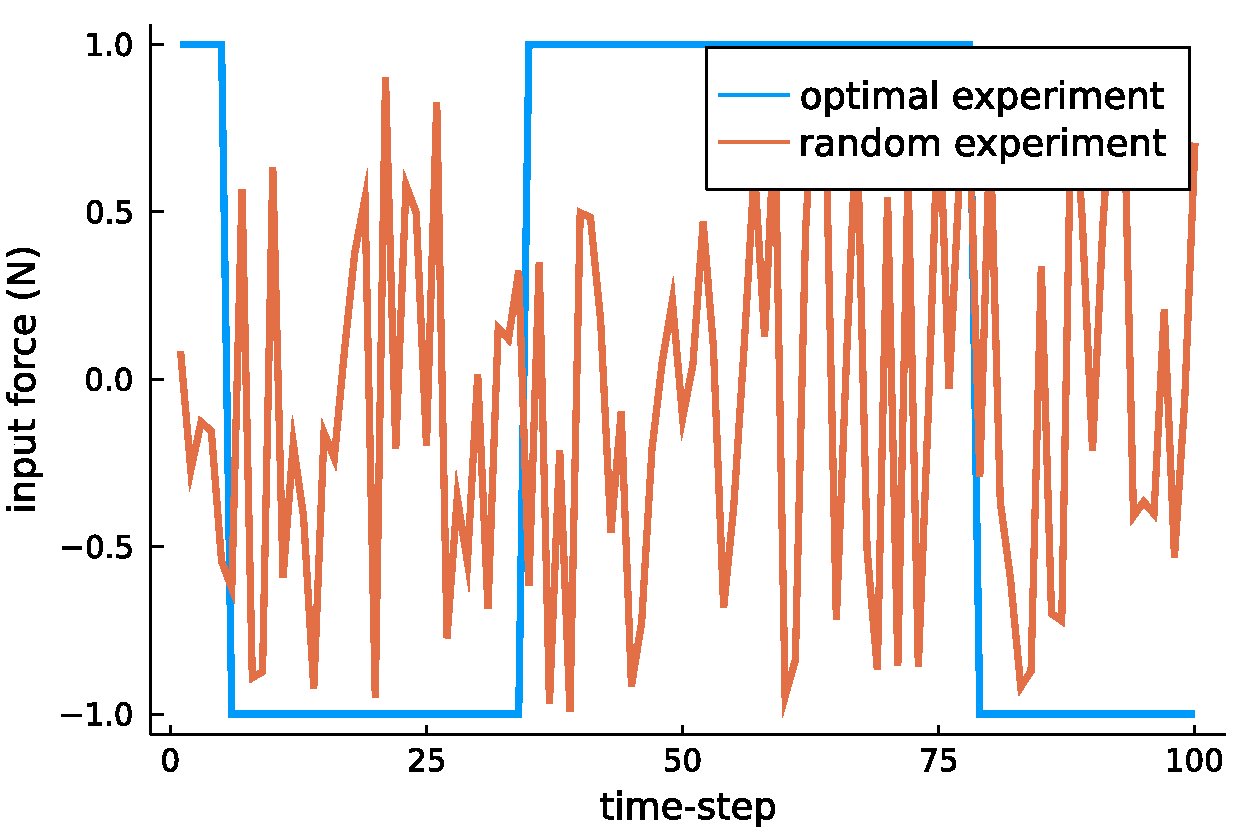
\includegraphics[width=1.0\textwidth]{figure/paper 3/optimal input}
		\caption{Input.}
		\label{figInput}
	\end{subfigure}
	\begin{subfigure}[b]{0.45\textwidth}
		\centering
		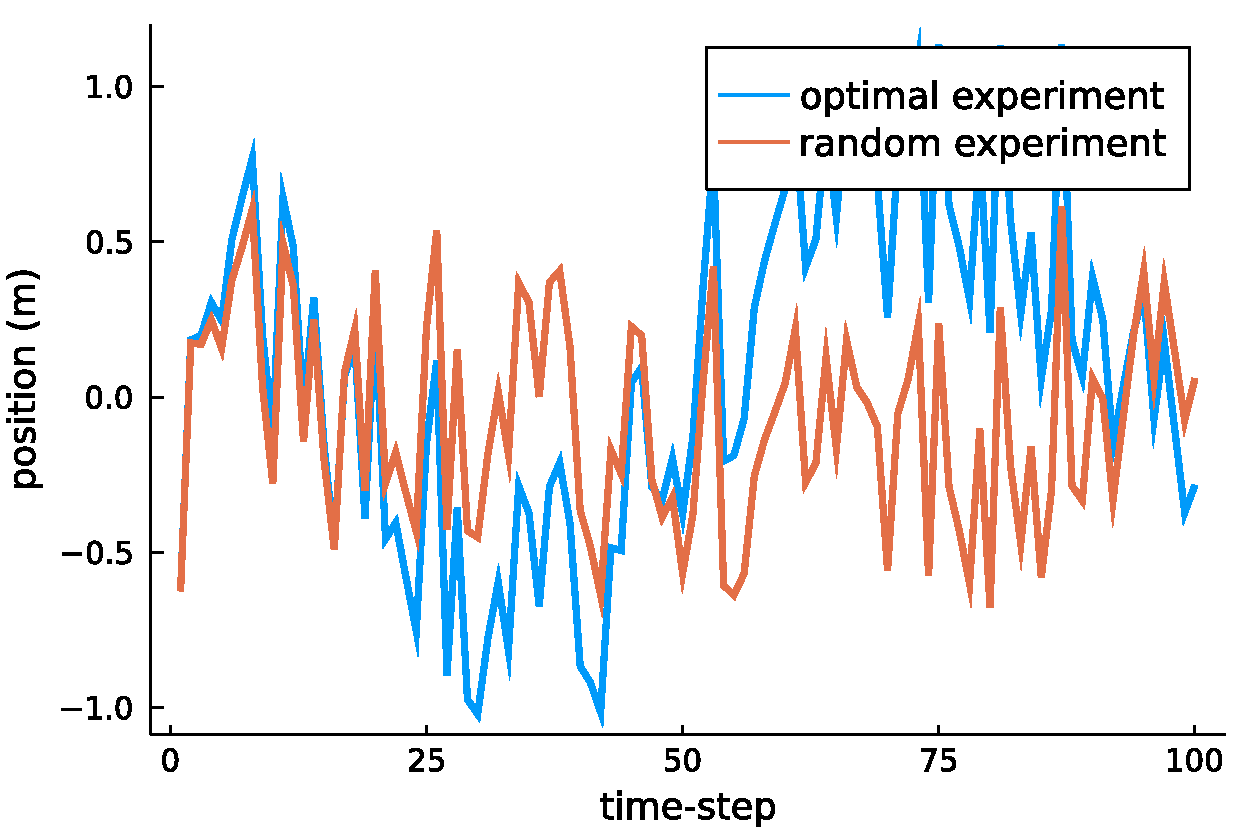
\includegraphics[width=1.0\textwidth]{figure/paper 3/optimal measurement}
		\caption{Output.}
		\label{figOutput}
	\end{subfigure}
	\caption{Comparison of optimal inputs compared to random inputs and the corresponding output behaviors.} 
\end{figure}
In Figure \ref{figOnline},  we show the evolution of the online maximum likelihood estimates as the experiment progresses. The optimal experiment hovers around the true model parameters after only $50$ time-steps, while the random experiment can not even correctly estimate these parameters after $100$ time-steps. The likelihood at the end of the experiment for the $100$ parameters drawn from the prior distribution for the model parameters is shown in Figure \ref{figLikelihood}. We see that the maximum likelihood estimate for the optimal experiment is one of the closest grid points to the true model parameter values, while this is not the case for the random experiment. Furthermore, for the optimal experiment the relative likelihood of other model parameters compared to the maximal likelihood estimate decreases rapidly when moving away from this estimate. This means that for the optimal experiment only model parameter values close to the true values fit the data well. For the random experiment the likelihood does not decrease rapidly when moving away from the maximum likelihood estimate, which means almost all values fit the data almost equally well and we can not discern the true model parameter values from the data.
\begin{figure}[H]
	\centering
	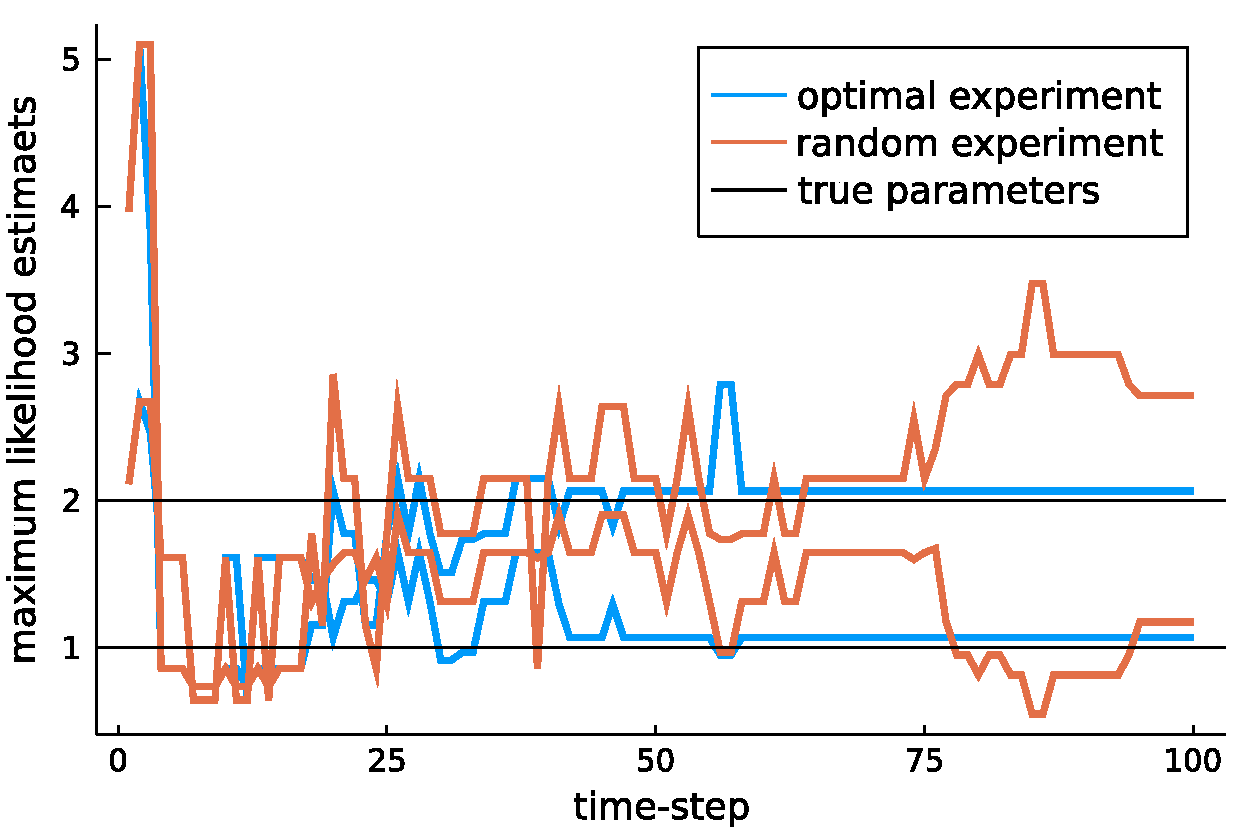
\includegraphics[width=0.8\textwidth]{figure/paper 3/online estimate}
	\caption{Online maximum likelihood estimates for both the optimal experiment and the random experiment. The optimal experiment converges faster to the true parameters.}
	\label{figOnline}
\end{figure}
\begin{figure}[H]
	
	\begin{subfigure}[b]{0.45\textwidth}
		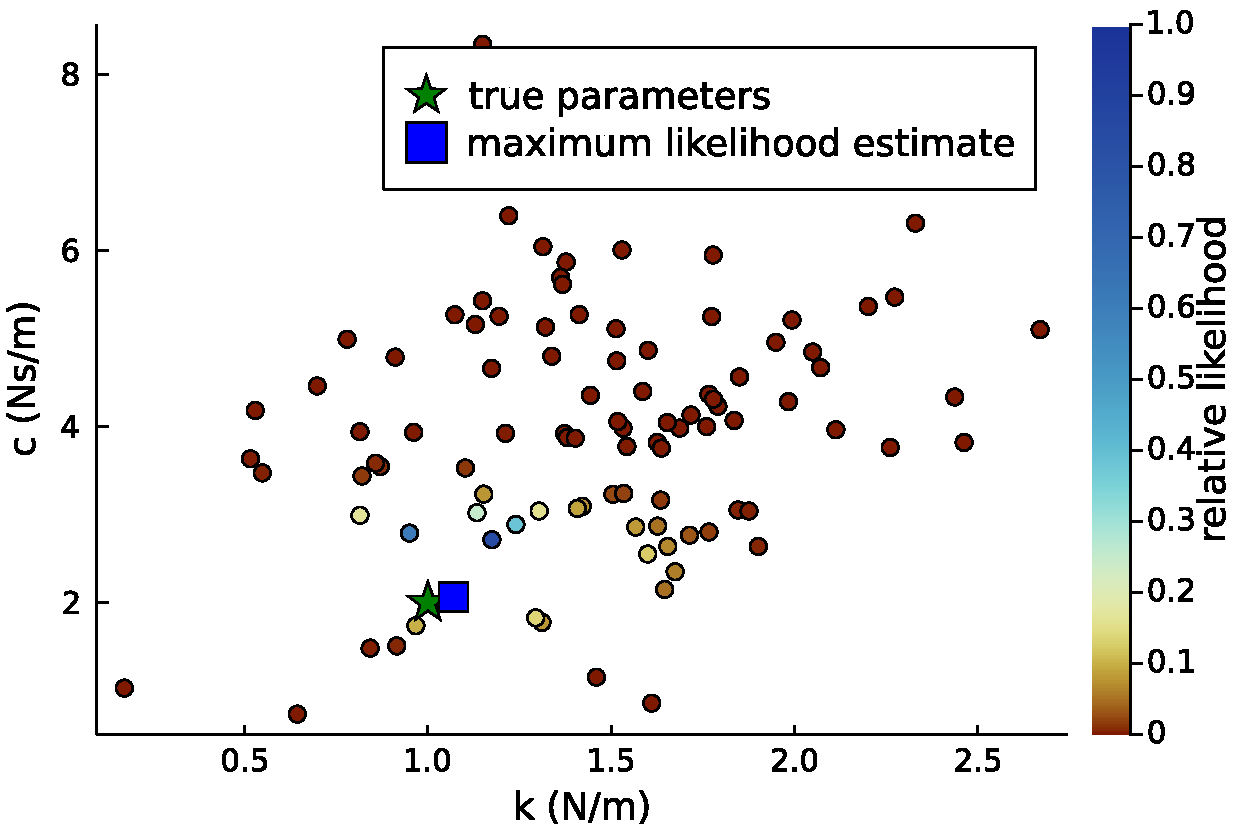
\includegraphics[width=1.0\textwidth]{figure/paper 3/likelihood profile optimal experiment}
		\caption{Optimal experiment.}
		\label{figLikelihoodOpt}
	\end{subfigure}
	\begin{subfigure}[b]{0.45\textwidth}
		\centering
		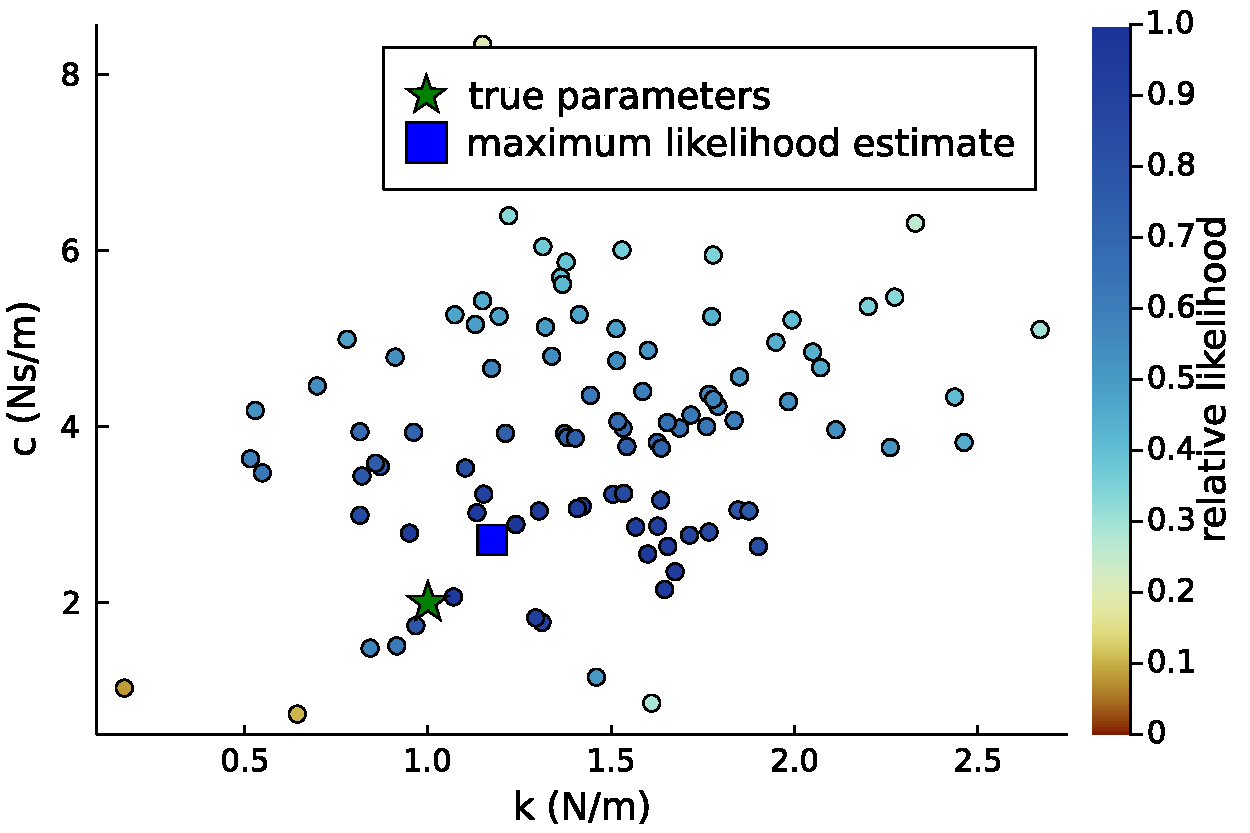
\includegraphics[width=1.0\textwidth]{figure/paper 3/likelihood profile random experiment}
		\caption{Random experiment.}
		\label{figLikelihoodRand}
	\end{subfigure}
	\caption{Likelihood grids at the end of the experiment. The likelihood decreases sharply away from the true parameters for the optimal experiment, unlike in the random experiment. The maximum likelihood estimate of the optimal experiment is much closer to the true value than the random experiment.} 
	\label{figLikelihood}
\end{figure}
\subsubsection{Added Value of the Robustness and Adaptivity}
The above discussion already shows the value of experimental design methodology compared to random inputs. We now continue by showing the combined added value of robustness and adaptivity. In Figure \ref{fig:analysis}, we study the behavior of Algorithm \ref{algo} for a variety of combinations of control horizon length $e$, number of model parameters drawn from the prior $N$, and number of time-steps, $T$. For each combination of $e$, $N$ and $T$ the experiment is repeated $100$ times and the mean and variance of the online maximum likelihood estimates are plotted. Figures \ref{figEnsembleOpt} and \ref{figEnsembleRand} show the same combination as was used before, in Figure \ref{figLikelihood}, for the optimal experiment and random experiment, respectively. This allows us to confirm that the optimal experiment performs much better than the random experiment over an ensemble of $100$ experiments, and, thus, that the better estimates of the experimental design methodology were not by chance.
\\
\\
In Figure \ref{figEnsembleRedHor}, the control horizon length, $e$, is reduced from $3$ to $1$. This causes this experiment to perform almost as bad as the random experiment. Increasing the control horizon length to $6$, however, does not greatly increase the performance of the experiment, as shown in Figure \ref{figEnsembleIncrHor}. Increasing the control horizon thus has diminishing marginal returns, which is good to know since a short horizon keeps the size of the matrices involved in the calculation of expected FIM in Equation (\ref{expectedFIMk}) manageable. The lack of additional information when increasing the control horizon is probably due to the increased variance of the predictions further into the future. 
\\
\\
The effect of the number of parameters drawn from the prior distribution, $N$, is shown in Figures \ref{figEnsembleRedRob} and \ref{figEnsembleIncrRob}. For the non-robust experiment, the mean of the prior distribution of the model parameters was used in the calculation of the Fisher information matrices in Equations (\ref{expectedFIMk}) and (\ref{observedFIM}), instead of a single random value from this distribution. The effect of reducing robustness is much less pronounced than the effect of reducing the control horizon. Only the convergence of the estimate of the damper constant is slower. Increasing the number of draws from the prior distribution from $100$ to $500$ also seems to have little added value past a certain point. This is because the Monte Carlo integration involved in Bayesian optimal design is already adequate.
\\
\\
We also compare our adaptive experimental design technique to the non-adaptive strategy from Equation (\ref{bayesian optimality}), in Figure \ref{figEnsembleNonAdp}. In the beginning of the experiment, the non-adaptive experiment performs equally well as our adaptive strategy. However, later on in the experiment, between time-steps $50$ and $75$, the estimation of the damper constant is clearly performing worse than the adaptive experiment. An additional shortcoming of the non-adaptive design is the large computational time required to generate this design. This is because the non-adaptive experiment requires predicting $100$ steps into the future. The optimization of this design was much slower than the adaptive designs with a short control window, due to the presence of large matrices in the expected FIM in Equation (\ref{expectedFIMk}).
\\
\\
Finally, the effect of a larger number of time-steps is shown in Figure \ref{figEnsembleIncrTime}. The Figure shows that, also here, there are diminishing marginal returns for longer experiments.
\begin{figure}[H]
	\begin{subfigure}[b]{0.45\textwidth}
		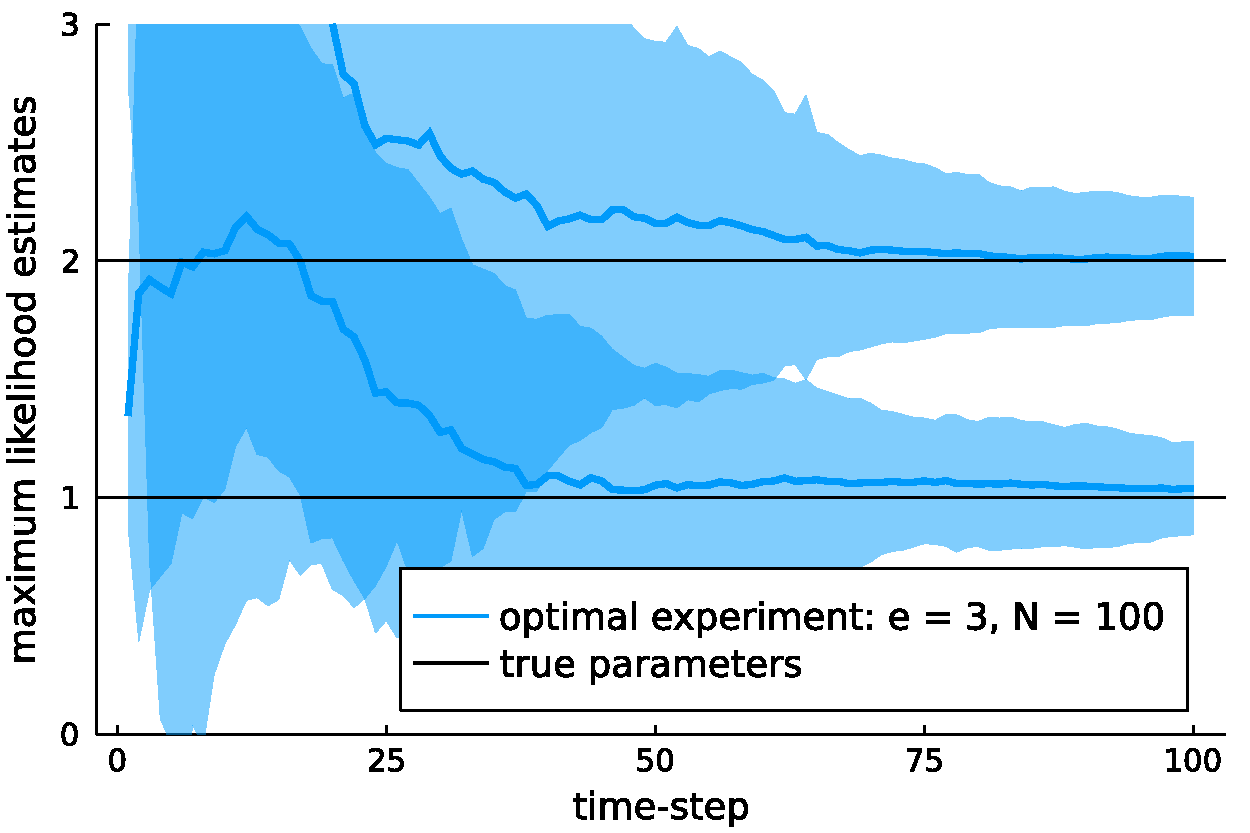
\includegraphics[width=1.0\textwidth]{figure/paper 3/ensemble online estimate optimal}
		\caption{Optimal experiment.}
		\label{figEnsembleOpt}
	\end{subfigure}
	\begin{subfigure}[b]{0.45\textwidth}
		\centering
		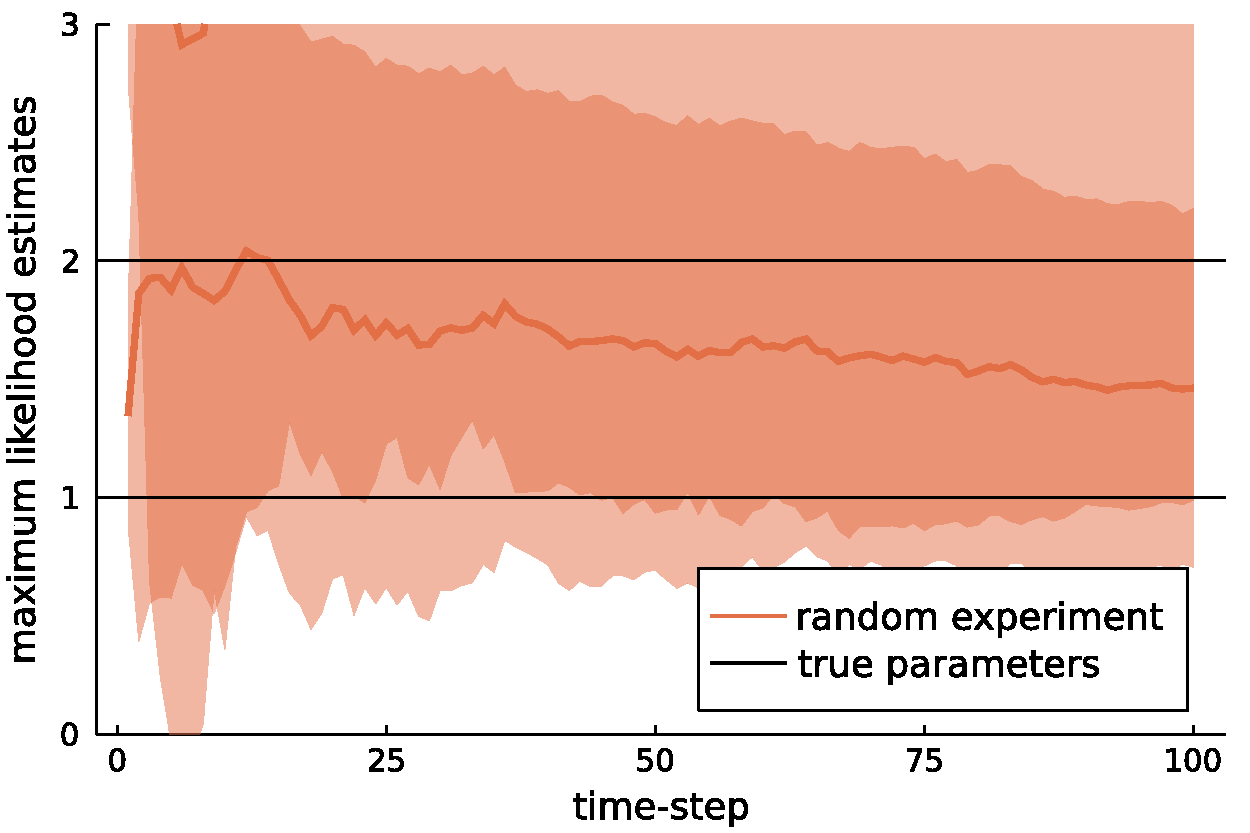
\includegraphics[width=1.0\textwidth]{figure/paper 3/ensemble online estimate random}
		\caption{Random experiment.}
		\label{figEnsembleRand}
	\end{subfigure}\\
	\begin{subfigure}[b]{0.45\textwidth}
		\includegraphics[width=1.0\textwidth]{figure/paper 3/ensemble online estimate reduced adaptivity}
		\caption{Reduced control horizon.}
		\label{figEnsembleRedHor}
	\end{subfigure}
	\begin{subfigure}[b]{0.45\textwidth}
		\centering
		\includegraphics[width=1.0\textwidth]{figure/paper 3/ensemble online estimate increased adaptivity}
		\caption{Increased control horizon.}
		\label{figEnsembleIncrHor}
	\end{subfigure}\\
	\begin{subfigure}[b]{0.45\textwidth}
		\includegraphics[width=1.0\textwidth]{figure/paper 3/ensemble online estimate reduced robustness}
		\caption{Non-robustness experiment.}
		\label{figEnsembleRedRob}
	\end{subfigure}
	\begin{subfigure}[b]{0.45\textwidth}
		\centering
		\includegraphics[width=1.0\textwidth]{figure/paper 3/ensemble online estimate increased robustness}
		\caption{Increased robustness.}
		\label{figEnsembleIncrRob}
	\end{subfigure}\\
	\begin{subfigure}[b]{0.45\textwidth}
		\includegraphics[width=1.0\textwidth]{figure/paper 3/ensemble online estimate non-adaptive}
		\caption{Non-adaptive experiment.}
		\label{figEnsembleNonAdp}
	\end{subfigure}
	\begin{subfigure}[b]{0.45\textwidth}
		\centering
		\includegraphics[width=1.0\textwidth]{figure/paper 3/ensemble online estimate increased time}
		\caption{Increased time.}
		\label{figEnsembleIncrTime}
	\end{subfigure}
	\caption{Mean and variance of online maximum likelihood estimates for different combinations of $e$, $N$ and $T$ in Algorithm \ref{algo}.} 
	\label{fig:analysis}
\end{figure}
\section{Two Compartment System}
In the second case study, we consider experimental design for a two compartment system. Compartment systems are common in postharvest modeling \parencite{lechaudel,yoneyama}, {\color{red}and pharmacokinetics \parencite{fedorov}}. The discretized linear dynamics of this system are:
\begin{equation}
\begin{aligned}
\bm x_k &= \begin{bmatrix}
1 - \Delta t(K_{1,0} + K_{1,2})  & \Delta tK_{2,1}\\
\Delta tK_{1,2} & 1 - \Delta tK_{2,1}
\end{bmatrix} \bm x_{k-1} +
\begin{bmatrix} \Delta t \\ \frac{\Delta t^2}{2}\end{bmatrix} u_k + 
\bm w_k,\\
\bm w_k & \sim  \mathcal{N}\left(\begin{bmatrix}0\\0\end{bmatrix},
\begin{bmatrix} q \Delta t & \frac{q\Delta t^2}{2} \\\frac{q\Delta t^2}{2}  &\frac{q\Delta t^3}{3} \end{bmatrix}\right),\\
y_k &= \begin{bmatrix} \Delta tK_{1,0} & 0 \end{bmatrix} \bm x + v_k, \\
v_k &\sim \mathcal{N}(0,0.0001).
\end{aligned}
\end{equation}
In these equations, $K_{1,2}$, $K_{2,1}$ and $K_{1,0}$ are the unknown model parameters that determine the flows between the two compartments and the flow from the first compartment to the environment. Their true values are assumed to all equal $0.2$. The prior distributions we use for them are independent normal distributions centered around $0.22$, with variances assumed equal to $0.0016$. The time between measurements, $\Delta t$, is assumed equal to $0.1$. The outflow of the first compartment to the environment is the measured output, with measurement noise on top of it. The initial distributions for the two compartments are assumed to be independent normal distributions with means equal to $10$ and $1$, and variances equal to $0.01$ and $0.00001$, respectively. The controllable input at time-step k, $u_k$, is a flow towards the first compartment. This input is constrained between $0$ and $10$. {\color{red}There is also an unknown stochastic input $\bm w_k$ to the first compartment, represented by a discretization of Brownian motion with spectral density $q$ equal to $0.001$. Brownian motion is a continuous time stochastic process whose increments are independent, stationary and normally distributed. The variance of the increments is determined by the spectral density.}
\\
\\
This example shows the added value of working with arbitrarily parametrized state space models, instead of linear autoregressive models. Some parameters, such as $K_{1,0}$, occur multiple times in the system dynamics. This is contrary to autoregressive models, where the output is assumed to be a linear combination of previous measurements and inputs, and each parameter of this linear combination is allowed to vary freely in the parameter estimation.
\\
\\
Figure \ref{figOnline2} depicts the progression of the online maximum likelihood estimate as time goes on. The optimal experiment was generated with $N=1000$ draws from the prior distribution, and looks $e=3$ steps ahead. The parameters are estimated precisely after roughly $50$ time steps, while the random experiment does not correctly estimate the model parameters even after $200$ steps.
\begin{figure}[H]
	\begin{subfigure}[b]{0.45\textwidth}
		\includegraphics[width=0.8\textwidth]{figure/paper 3/online estimate2opt}
		\caption{Optimal experiment.}
	\end{subfigure}
	\begin{subfigure}[b]{0.45\textwidth}
		\includegraphics[width=0.8\textwidth]{figure/paper 3/online estimate2rand}
		\caption{Random experiment.}
	\end{subfigure}
	\caption{Online maximum likelihood estimates for the two compartment model.}
	\label{figOnline2}
\end{figure}
\section{Discussion and Conclusion}
In this chapter, we presented a novel robust and adaptive experimental design method to estimate the model parameters of discrite-time linear state space models. We achieved this by quantifying the information content of an experiment using a combination of the expected and observed Fisher information matrix. In future research, we want to extend these results to non-linear dynamics. The Kalman filter must then be replaced with another Bayesian filter, such as the extended Kalman filter, sigma-point filter or particle filter. Continuous-time dynamics is another interesting direction for future research, as almost no literature exists on experimental design for stochastic differential equation models.
\\
\\
To be able to optimize our experiments adaptively, we were forced to evaluate the likelihood of the model parameters at the same location (in the model parameters space) at every time-step. Most locations quickly become very unlikely, as seen in Figure \ref{figLikelihoodOpt}. It would be better if this sample could slightly move towards regions of higher probability at every time-step. \textcite{kantas} give an overview of methods that allow for such jittering of the location of the model parameters, but none of the methods discussed are completely online. Since these authors are only interested in online parameter estimation, this is not a major issue for them. But when also considering adaptive experimental design, where an optimization over the input space has to be ran at every time-step, the jittering of the model parameters must be very efficient. Very recently \textcite{he}, published a promising method for online parameter estimation for linear dynamic systems based on the Kalman filter, that could be used for this purpose, and which we plan to incorporate in future research.
\chapter{Conclusion and Outlook}
\label{conclusion}
\section{Overarching Conclusion}
The general goal of this thesis is to show the usefulness of dynamic experiments for {\color{red}bio-engineering} applications. The case studies in Chapters \ref{paper1} and \ref{paper2} {\color{red}focus on postharvest modeling and} show that dynamic experiments indeed lead to a much more precise {\color{red}and robust} estimation of respiration and fermentation parameters of pear fruit with reduced experimental effort. {\color{red} Chapter \ref{paper3} focuses on experimental design methodology for linear dynamical systems in the presence of process noise. This methodology leads to improved experiments for models commonly used in bio-mechanics and pharmacokinetics.}
	
	To reach this general goal, multiple challenges had to be overcome:
	\begin{itemize}
		\item \textbf{Challenge 1}: The optimal experiment depends on the true values of the model parameters which the experiment aims to learn about. Some form of prior information about these parameters is thus always required to begin optimizing the experiment. In \textbf{Chapter \ref{paper1}}, we solved this issue by taking parameter estimates from the literature and used them to construct locally optimal designs. Using this methodology, experiments to estimate Michaelis-Menten respiration parameters for pear fruit were constructed. These experiments perform better than heuristic techniques used in postharvest experimentation.
		\item \textbf{Challenge 2}: Robust experimental designs perform well over a wide range of possible parameter values. Bayesian experimental design is a popular technique to achieve robustness, where the prior information is quantified using a probability distribution. The design is then optimized to perform well on average, where the information content is averaged over this prior distribution. Available Bayesian experimental design techniques from the literature only allow for parametric distributions to quantify this prior information, and these techniques were found to be insufficient to adequately describe the prior information we had available for the respiration and fermentation of pear fruit. In \textbf{Chapter \ref{paper2}}, an experimental design methodology was developed that can deal with arbitrary prior distributions obtained by using a Markov-Chain Monte-Carlo integration technique. This methodology was then found to perform better than the traditional locally optimal design method used in \textbf{Chapter \ref{paper1}}. {\color{red}It was also demonstrated to perform better than other robust experimental design methods, that use parametric distributions as prior information.} This methodology was then used to construct robust experiments to estimate the respiration and fermentation of pear fruit.
		\item \textbf{Challenge 3}: Little experimental design literature exists on how to deal with dynamic systems with both process and measurement noise. In \textbf{Chapter \ref{paper3}}, the Fisher information matrix (FIM) is derived for linear dynamical systems with both kinds of noise. {\color{red}The use of this FIM in an experimental design context is new to the literature}. The key discovery here is that experimental design for dynamic systems with hidden dynamic states requires tracking these hidden states using an appropriate Bayesian filter, which for linear systems equals the Kalman filter.  
		\item \textbf{Challenge 4}: Adaptive experimental design techniques are needed when the prior information about model parameters is poor. These adaptive techniques re-optimize the remainder of the experimental design after every measurement. However, the optimization problem that occurs in the traditional experimental design technique, which is based on the expected Fisher information matrix, keeps growing in complexity at every time-step. In \textbf{Chapter \ref{paper3}}, this issue is solved by developing a novel experimental design criterion based on a combination of the observed and expected FIM. The observed FIM is computationally less expensive as it only utilizes the actually observed measurements, thus making it well suited for quantifying the information from the already gathered measurements. The expected FIM requires an expectation over all possible observations, making it well suited to quantify the information of future observations. A combination of these two types of Fisher information matrices results in an experimental design methodology that requires the same amount of computation at every time-step, which is a necessity for adaptive experimental design. {\color{red} Such a combination of the observed and expected FIM has not yet been used for dynamic experimentation.}
	\end{itemize} 
\section{Outlook}
In this thesis, I developed novel experimental design methodology for dynamic systems. I believe that more interesting and important research can still be done in this area, including research on experimental design methodology for more complicated dynamic models, novel ways to quantify uncertainty and more efficient numerical techniques. In this section, I discuss some possible perspectives on future research.
\subsection{Model Selection}
It is commonly assumed in the experimental design literature that the entire model structure is known. However, it is often more realistic that:
\begin{itemize}
\item Competing model structures exist to explain a certain phenomenon.
\item Only part of the model structure is known, and there are missing components in the model.
\end{itemize}
Appropriate experimental design techniques should be developed that can deal with both model parameter and model structure uncertainty.
\subsubsection{Model Discrimination}
Some experimental design techniques for model discrimination in dynamic systems exist \parencite{chen}, mostly based on the Hunter and Reiner criterion \parencite{hunter}. A weakness of this approach is that it is not robust, since it does not account for parameter uncertainty. Instead, the method only compares models at point estimates of the parameters. If there is much parameter uncertainty, the Hunter and Reiner method will be overly optimistic in its ability to discriminate models. Instead of this method, a Bayesian optimal design method, similar to the one used in Chapter \ref{paper2}, could be developed, where an information criterion, averaged out over a joint prior distribution for the model structure and the model parameters, is optimized. The challenge here is to generalize the Markov-Chain Monte-Carlo integration technique to deal with both the continuous model parameters and the discrete model structures. 
\subsubsection{Missing Model Components}
Another form of model uncertainty occurs when only part of the model structure is known. One method to deal with missing model components is to replace them with a black box model, such as a Gaussian process or neural network. Replacing parts of a differential equation with a surrogate model is currently a hot topic within machine learning \parencite{rackauckas3,rackauckas4}. Optimal experimental design techniques have not been used by machine learning communities, as they often deal with large observational datasets. However, when combining the black box modeling approach from machine learning and mechanistic models for biological systems, in scenarios where acquiring experimental data is cumbersome and time-consuming, there is a need for carefully crafted experiments. Instead of quantifying the uncertainty of a finite dimensional parameter space, here the challenge lies in quantifying the uncertainty of an infinite dimensional function space. To achieve this, methodological concepts from optimal design of computer experiments can be borrowed, where the Fisher information and entropy based criteria have already been combined with Gaussian processes \parencite{santner}. Of course, computer simulations are often deterministic, while biology is rife with variability.
\\
\\
Throughout this thesis we assumed that Michaelis-Menten reaction kinetics perfectly summarize the respiration and fermentation behavior of pear fruit. However, in reality this is just a summary of a much larger biological pathway, and diffusion also plays a role, leading to a high dimensional partial differential equation model. Instead of working directly with this more complicated model, the misspecification on the lumped model could be taken into account through a Gaussian process \parencite{kennedy}, but experimental design for such misspecified systems has not yet been considered in literature.
\subsection{Process Noise}
In chapter \ref{paper3}, I developed an experimental design method to deal with process noise for discrete-time linear dynamical systems. For such systems, the Fisher information matrix has a tractable form, involving the Kalman filter to estimate the hidden state. The next step here is replacing the linear dynamics with non-linear dynamics. The Kalman filter then no longer suffices to estimate the hidden state. A more complicated filter, such as an extended Kalman, unscented or particle filter must then be used, greatly increasing the computational cost. If we then also consider continuous time models, we arrive at the unexplored research topic of experimental design for stochastic differential equation models.
\subsection{Kullback-Leibler Divergence}
In this thesis, I used the Fisher information matrix (FIM) to quantify the information content of an experiment. The Kullback-Leibler divergence (KL-div) is another method to quantify the information content. Unlike the FIM, the KL-div does not involve normal approximations, and might be a better criterion for small sample sizes. The major drawback is that the KL-div is numerically much more intensive to calculate.  This is generally done using a double loop Monte-Carlo integration method \parencite{ryan}. Recently, advances have been made in lowering the computational burden of the KL-div based approach by considering variational Bayesian techniques \parencite{foster}, where the inner Monte-Carlo loop is replaced by optimizing a variational distribution. This technique then allows for jointly optimizing the design and variational parameters \parencite{foster2}.
\subsection{Koopman Expectation}
In Chapter \ref{paper2} of this thesis, we calculated the expectation required for Bayesian experimental design by pushing forward the uncertain extended state distribution in time, and then calculating some quantity of interest at each time point. \textcite{gerlach} recently proposed a new method to calculate expectations for dynamic systems that instead pulls back this quantity of interest in time, using the Koopman operator which relies on the change of variable formula. This idea is analogous to the back propagation (adjoint sensitivity analysis) of gradients for optimization. Calculating the expectation using the Koopman operator is thus generally a good choice when a low number of expectations have to be calculated, such as the expectation of a scalar function as opposed to the expectation of a vector function. In Bayesian experimental design, such an expectation of a scalar function of the FIM is calculated. This means calculating the expectation using the Koopman operator should be favorable from a computational cost perspective. 
\subsection{Fully Risk Averse Experimental Design}
In this thesis, we took an expected value approach to deal with uncertainty, in the sense that uncertainty on the model parameters was quantified using a probability distribution, and experiments were optimized for the average of an information criterion over this distribution. Experimental design techniques that instead assume a worst case scenario for the model parameter uncertainty also exist, such as the techniques developed by \textcite{bauer}. Here, the experimental design is optimized for the minimum of an information criterion over the set of possible model parameters. This method, however, only uses the worst case scenario to deal with parameter uncertainty, but there is, of course, also uncertainty in the measurements, and other model disturbances such as process noise. If these errors are bounded, we can also assume a worst case scenario here. There exist parameter estimation techniques that produce the entire set of model parameters that are consistent with the measurements, while eliminating those that are not possible \parencite{jaulin}. However, these set based techniques have only recently been used for experimental design \parencite{jauberthie}. It would in particular be interesting to combine these methods with reachability analysis for dynamic systems \parencite{juliareach}, which are techniques to numerically solve differential equations, which return a tube in which the true solution is guaranteed to exist. Fully risk averse experimental design techniques would particularly be of interest for designing experiments that guarantee the true model parameters lie within a set of a chosen size.  
\subsection{Goal Driven Experimental Design}
Most experimental design literature for dynamic systems focuses on a precise estimation of all model parameters, putting equal importance on each parameter. Often, the reason for estimating the model parameters is to use the resulting model in the control and optimization of the bioprocess. To achieve an optimal control or to find the optimal input settings for a bioprocess, not all model parameters are equally important. Instead, it is typically a non-linear function of a subset of the model parameters that matters. More effort should therefore be spent on precisely estimating the relevant functions of the influential parameters. The challenge here is transforming the variability of the parameters into a variability of optimal operation levels. Experiments then must be constructed to minimize this latter uncertainty.
\\
\\
This topic of precisely estimating a non-linear function has only been briefly explored in the dynamic experimental design literature, more specifically by \textcite{houska}. These authors started by using the Fisher information matrix to quantify the uncertainty about the model parameters and then linearize the effect that the model parameters have on the optimal conditions and transform the parameter uncertainty into an uncertainty on the optimal conditions, using the delta method. However, they did not use this technique to find an optimal point in the design region, which would be a particularly interesting application of this technique. \textcite{li} suggested a method to achieve this, but only for generalized linear models. Their method splits the Kullback-Leibler divergence into two parts: (i) the Kullback-Leibler divergence between the observations and the unknown parameters, and (ii) an information loss term between the unknown parameters and the optimal conditions quantified by the data processing inequality theorem \parencite{cover}. However, this technique has not yet been used in combination with dynamic systems.

\appendix
\chapter{Markov chain details} 

 \begin{table}[H]
 	\caption{100 elements of Markov-chain points used to generate robust designs in Chapter \ref{paper2}}
 	\npdecimalsign{.}
 	\nprounddigits{3}
 	\footnotesize 
 		\begin{tabular}{c c c c c c}
 		$V_{\text{m},\oxy}$&\quad $K_{\text{m},\oxy}$ & \quad $K_{\text{mn},\text{CO}_2}$ & \qquad\quad $r_q$ &\qquad $V_{\text{m,f,}\coxy}$ & \quad $K_{\text{m,f},\oxy}$\\
 		\hline
 		$\mu$mol$\text{ kg}^{-1}$ $\text{ s}^{-1}$ & \quad kPa & \quad kPa & \qquad \quad - & \qquad $\mu$mol$\text{ kg}^{-1}$ $\text{ s}^{-1}$& \quad kPa \\ 
 		\hline
 	\end{tabular}
 	\begin{tabular}{n{5}{5}n{5}{5}n{5}{5}n{5}{5}n{5}{5}n{5}{5}}
 		0.318508614331184 & 6.04815595974601 & 1509.96536884989 & 0.660445389919239 & 0.120064905458288 & 0.218736644322706 \\
 		0.3366765302209   & 6.4989446794794  & 360.727888868205 & 0.646614996449114 & 0.118243450257619 & 0.261775301445684 \\
 		0.302102552888642 & 4.12710679843391 & 381.99844715205  & 0.660206364648354 & 0.122667798576189 & 0.158253068991815 \\
 		0.314219308134651 & 5.37562876842769 & 1879.10690696227 & 0.664542853132253 & 0.122443862238542 & 0.213095203612259 \\
 		0.31833781623091  & 6.07958734167217 & 705.206104742112 & 0.660120621845056 & 0.118702858163443 & 0.245176644829309 \\
 		0.320126665973657 & 5.97324099684699 & 547.185787448147 & 0.653518325371884 & 0.119435686657796 & 0.248213427685774 \\
 		0.325016539016138 & 6.07465441035316 & 613.317817278808 & 0.656640094462975 & 0.122284988649866 & 0.225967087667975 \\
 		0.333153514230406 & 6.30265999426891 & 3993.31903940915 & 0.652191508844257 & 0.122134039188995 & 0.249003696541361 \\
 		0.31522529029466  & 4.73542681592021 & 151.390183345118 & 0.65676016412844  & 0.122811223260368 & 0.194561418370892 \\
 		0.334506187134661 & 6.45661508570156 & 1880.45424625504 & 0.648600756151934 & 0.121229158855321 & 0.248172522119006 \\
 		0.31836015117952  & 5.96842768712396 & 486.79081219096  & 0.657006108305125 & 0.121260566888754 & 0.25471010118915  \\
 		0.314858697751157 & 4.92684204574587 & 116.835225378422 & 0.66677844617737  & 0.121675443871356 & 0.211536231802224 \\
 		0.314437049526582 & 5.21890243482379 & 668.049659817922 & 0.656110681788805 & 0.121717450379592 & 0.198876092588128 \\
 		0.300588278046269 & 4.77866922456738 & 2834.25289533835 & 0.654504857803367 & 0.122418056320972 & 0.203092758963978 \\
 		0.315079856317089 & 4.87486140410768 & 524.641337087368 & 0.65234009401046  & 0.121189082600876 & 0.206686261164657 \\
 		0.325220432361288 & 5.43213694681068 & 206.58294577159  & 0.655810719998244 & 0.121526622712228 & 0.200430403716489 \\
 		0.31791718331981  & 5.79598900154415 & 4876.47942990697 & 0.664225083205325 & 0.118896713043982 & 0.217892655461518 \\
 		0.321342417759747 & 5.46534119886633 & 866.088622630029 & 0.650193263867793 & 0.118824907511037 & 0.194304316100639 \\
 		0.315905771577064 & 5.48701887597961 & 626.560976729637 & 0.651174642251753 & 0.120587678662095 & 0.232612375348884 \\
 		0.30183798834681  & 4.51106854828106 & 1211.47569258765 & 0.651760116662972 & 0.119656923164515 & 0.18518590636603  \\
 		0.313293163525632 & 5.46786176130965 & 1396.07257762323 & 0.660598561875813 & 0.121061222132764 & 0.207397845241727 \\
 		0.330560722389421 & 5.75558164310123 & 361.898758986167 & 0.646198492275519 & 0.121681326759503 & 0.25296554026459  \\
 		0.331969595155542 & 6.10152921124937 & 519.658600427234 & 0.665150399363897 & 0.117742167316981 & 0.202575346494747 \\
 		0.306202665955883 & 5.2707622034866  & 2050.85743406461 & 0.66283120117732  & 0.121195006578131 & 0.184355535572427 \\
 		0.325574588548857 & 5.58224196241912 & 198.513825204249 & 0.662814187162619 & 0.121824990371076 & 0.233810238458072 \\
 		0.32647078589132  & 5.77731677384858 & 351.813387290949 & 0.655491946507297 & 0.121513179645681 & 0.230009143523411 \\
 		0.322440262561728 & 5.46209724307101 & 803.831811838077 & 0.648257488709801 & 0.119839147816655 & 0.213326591936953 \\
 		0.318114949722254 & 5.38255153008611 & 271.911285788239 & 0.655890179821892 & 0.121040554561676 & 0.214947962308283 \\
 		0.326186231995068 & 5.67514341757284 & 399.560808455696 & 0.644904522558664 & 0.121196588107287 & 0.236228184694665 \\
 	\end{tabular}
\end{table}
 \begin{table}[H]
	\npdecimalsign{.}
	\nprounddigits{3}
	 	\footnotesize 
	\begin{tabular}{n{5}{5}n{5}{5}n{5}{5}n{5}{5}n{5}{5}n{5}{5}}
		0.332041961082678 & 6.14757824879231 & 372.445934852407 & 0.647116106402099 & 0.122115486331076 & 0.245489000458452 \\
		0.317652979939013 & 5.31006746428385 & 2123.00329174392 & 0.649004694201989 & 0.120033051163376 & 0.222048255556139 \\
		0.309182843084995 & 5.1366899794342  & 30722.2402444234 & 0.645740388382136 & 0.120933176586695 & 0.218782712444288 \\
		0.327520115734193 & 5.60042617863142 & 498.991192143013 & 0.645791852081752 & 0.121594129999007 & 0.223952677768808 \\
		0.317213949634944 & 5.98139851405716 & 672.747745261585 & 0.666559071285828 & 0.117920340356643 & 0.234882628605402 \\
		0.320176606281803 & 5.79615164967532 & 1353.34789686553 & 0.65675137407904  & 0.120062472489838 & 0.225647095302847 \\
		0.334831719244313 & 6.16321314201174 & 4266.78554603494 & 0.649889894822226 & 0.11882037693595  & 0.257597673267609 \\
		0.32915546669441  & 6.39781451544468 & 566.697368290348 & 0.667800786292786 & 0.120954159834197 & 0.215053057088096 \\
		0.327893339317489 & 5.79676424274502 & 1096.3127412216  & 0.640660081602347 & 0.121233746827497 & 0.274758400052423 \\
		0.30910358430459  & 5.04553191131639 & 270.633217089987 & 0.670119206486157 & 0.119351775175732 & 0.185880147683897 \\
		0.317224772479636 & 5.61891030769034 & 1594.17082717433 & 0.659361346311357 & 0.120889620725134 & 0.222941205373158 \\
		0.315192785690751 & 5.64474586227631 & 669.299331407436 & 0.657138336339387 & 0.119799165799614 & 0.213593683866381 \\
		0.321262858259361 & 5.0869258369163  & 158.819196457117 & 0.656388718859759 & 0.117583757249923 & 0.218162733209615 \\
		0.313310378735151 & 4.9382333338299  & 663.970009620958 & 0.659414553373868 & 0.118375393964668 & 0.189346771772704 \\
		0.328461603117464 & 6.04505323480272 & 247.833988150921 & 0.660253506474548 & 0.121738391981482 & 0.252465879323468 \\
		0.349022187696091 & 6.20107268766493 & 311.905926885716 & 0.64651229818088  & 0.120862966024437 & 0.266496660240059 \\
		0.296554035743576 & 4.98551876985716 & 898.950644471995 & 0.672996055823689 & 0.122308695488948 & 0.192986637658905 \\
 		0.311460542970216 & 5.41402448139344 & 8614.48564695176 & 0.655353840892296 & 0.120420300784372 & 0.258008414682011 \\
 		0.320496802316695 & 5.57128733572169 & 378.320393351686 & 0.648486525730796 & 0.1217033371611   & 0.243506572528154 \\
 		0.304692398387076 & 5.50676884500111 & 18510.4099102035 & 0.660652025442697 & 0.121395559037202 & 0.220232725957306 \\
 		0.324622146497338 & 5.90570240829214 & 799.308829408022 & 0.655461080139648 & 0.120922868218464 & 0.235121239372157 \\
 		0.327111187453926 & 5.9991913440585  & 1192.22698426794 & 0.659284611573014 & 0.123200585052002 & 0.215040838352831 \\
 		0.31879620704631  & 5.34331133277902 & 256.174782464711 & 0.650948201014754 & 0.123614313904772 & 0.231926943604941 \\
 		0.315439631941733 & 5.44039329512793 & 1012.41151455344 & 0.659480364317243 & 0.122260078515923 & 0.204707635027967 \\
 		0.308997940141195 & 4.56747606072807 & 1305.07691642274 & 0.632485290098387 & 0.119981223509041 & 0.199842707240371 \\
 		0.313029433454973 & 5.52980847192066 & 866.166709553468 & 0.652621176285811 & 0.120700074494617 & 0.217319696918995 \\
 		0.30927452629547  & 5.32057002440216 & 1812.79203145514 & 0.656540888327628 & 0.121990398440631 & 0.232155983545142 \\
 		0.320073392687525 & 5.38936967464446 & 448.156188564658 & 0.66320736016339  & 0.119584475169863 & 0.21563939924248  \\
 		0.311300000024136 & 5.2707435400272  & 782.165663191959 & 0.658299408325193 & 0.120118456202829 & 0.217295178887021 \\
 		0.348350538364642 & 6.59778378007261 & 263.405535245219 & 0.649188061149773 & 0.122279157844779 & 0.27513674091538  \\
 		0.312690905543397 & 5.53678299132432 & 1784.75256996726 & 0.663381078401136 & 0.119601130528535 & 0.2170705037326   \\
 		0.320717384914297 & 5.73405802745756 & 300.29787664852  & 0.662338890940346 & 0.121957460167126 & 0.20242793231183  \\
 		0.309652567207312 & 5.04724719565912 & 187.940923042166 & 0.657545583191208 & 0.121949930479354 & 0.209744277614292 \\
 		0.329713619598733 & 6.20565490139954 & 664.202502702332 & 0.658808849021428 & 0.118889079487233 & 0.217965549502044 \\
 		0.33850905163201  & 5.82236127818076 & 194.899656197645 & 0.649928291664766 & 0.119413175017138 & 0.227339725608901 \\
 		0.32668780266818  & 5.89988799188929 & 5201.3938212032  & 0.639251366010453 & 0.119247910979903 & 0.231019867023812 \\
 		0.314571081650472 & 5.17783071008396 & 254.046422543519 & 0.657730606261981 & 0.121582287221685 & 0.200679670423195 \\
 		0.321062951844899 & 5.5634407053792  & 954.128012530614 & 0.642126669563546 & 0.122371756551465 & 0.235563554919541 \\
 		0.313476291581249 & 5.27703280471457 & 863.780102876026 & 0.645904576047482 & 0.120871189312146 & 0.231470537697429 \\
 		0.294294638285352 & 4.65956867514367 & 10601.0537024113 & 0.642993184538469 & 0.121425299235935 & 0.208445068409166 \\
 		0.32295508644707  & 5.54927254601265 & 47663.9432076052 & 0.649064437724597 & 0.120750753118487 & 0.21474502092144  \\
 		0.316409515709253 & 5.37378253667922 & 826.334261279306 & 0.657152507584127 & 0.122073282674412 & 0.19403864224379  \\
 		0.332273540451094 & 6.34599067309403 & 590.861452727395 & 0.660201221524623 & 0.121952022563632 & 0.248807519718328 \\
 		0.324140319763945 & 6.54427517593076 & 2189.37208560683 & 0.65609508072423  & 0.120760932259044 & 0.266472391996216 \\
 \end{tabular}
 \end{table}
 \begin{table}[H]
	\npdecimalsign{.}
\nprounddigits{3}
\footnotesize 
	\begin{tabular}{n{5}{5}n{5}{5}n{5}{5}n{5}{5}n{5}{5}n{5}{5}}
 		0.320705211065065 & 5.57112633720428 & 390.298964741531 & 0.6498917074742   & 0.122390546646592 & 0.206535744783911 \\
 		0.327506217987222 & 5.70712037231452 & 530.657247964027 & 0.649811661081613 & 0.121309840109408 & 0.251432131225708 \\
 		0.320119087003615 & 5.23380804438769 & 898.43442606263  & 0.64979588086811  & 0.121640050485195 & 0.223189206534877 \\
 		0.333175632345002 & 6.07510917677871 & 280.155522374373 & 0.663927489035827 & 0.120736203839222 & 0.215325529107837 \\
 		0.322115516941283 & 6.31840324055752 & 1230.35989696967 & 0.655740341476626 & 0.120256439713467 & 0.248911545938515 \\
 		0.325217660826441 & 5.73199057461668 & 525.615471043276 & 0.653502037894899 & 0.120678592590833 & 0.232719235668256 \\
 		0.313720967173929 & 5.54315458520584 & 1315.74085284859 & 0.651026442233558 & 0.121265402177748 & 0.191333126831378 \\
 		0.323654365799897 & 5.60022199163021 & 885.67227643849  & 0.654788687861854 & 0.118238771119867 & 0.218390258047143 \\
 		0.295357831386373 & 4.89831197458082 & 4308.87287480727 & 0.66446131726132  & 0.122504521175691 & 0.190091690175004 \\
 		0.324642337508802 & 6.0192077956125  & 463.202351075915 & 0.672869027168013 & 0.123649091230809 & 0.209736587923553 \\
 		0.319690814583472 & 6.08844412211424 & 589.509552623018 & 0.665617369613351 & 0.121369843632552 & 0.212585158443716 \\
 		0.322049681941771 & 5.7430399630277  & 3817.62883927908 & 0.654706659875394 & 0.120357842004168 & 0.229118942761571 \\
 		0.315567729902975 & 5.66867280559779 & 2696.07477745296 & 0.641725452369799 & 0.120701214408872 & 0.252511873019668 \\
 		0.332517304032212 & 5.81897253904527 & 464.96043880316  & 0.655705106103049 & 0.121125459181873 & 0.242827826408568 \\
 		0.314696416537925 & 4.84247713947164 & 366.879879128163 & 0.665787571371491 & 0.119436683814609 & 0.183326270718402 \\
 		0.317393048178107 & 5.48691862159227 & 8669.23679445632 & 0.662154658566078 & 0.120004387134531 & 0.20212505315148  \\
 		0.304314848261041 & 4.37198961573627 & 130.305529675171 & 0.672930563572603 & 0.122967403414143 & 0.16951967207738  \\
 		0.31695712311361  & 5.22666195718183 & 857.620826939289 & 0.638588448896424 & 0.120895233668943 & 0.243126665758576 \\
 		0.342691822535571 & 5.83731452533875 & 116.377794537394 & 0.664076265955428 & 0.118245894875147 & 0.250353105254969 \\
 		0.309667360861597 & 5.17490822682801 & 501.003421285926 & 0.661758035068401 & 0.120218991921796 & 0.240922012980486 \\
 		0.325207433735219 & 5.52021985360655 & 432.655537244372 & 0.647002912414558 & 0.121624906245272 & 0.230228268712523 \\
 		0.313401417722865 & 5.10794797647781 & 308870.950285741 & 0.64818746525688  & 0.121579720775784 & 0.209975243550797 \\
 		0.311681441611968 & 5.60353713430749 & 829.500902415609 & 0.653365660955094 & 0.121794465743355 & 0.232462487646987 \\
 		0.338037756382311 & 6.57237875056282 & 3040.24106528456 & 0.63790121065451  & 0.119083657754214 & 0.264296033172469 \\
 		0.314938196891838 & 5.56884270214538 & 132026.341990687 & 0.644376424279895 & 0.123024588722495 & 0.230928502971933 \\
 		0.301399836458591 & 5.04180349148716 & 2842.4647341608  & 0.667210094497958 & 0.12065035675556  & 0.182125726571677 \\
 		0.312849740863458 & 5.45171374528387 & 8565.54476965598 & 0.676610394118923 & 0.120422063092985 & 0.191405360103286
 	\end{tabular}
 \end{table}
\cleardoublepage


\backmatter

% BibLatex (comment lines above and comment out biblatex lines in preamble)
\printbibliography
\chapter*{Publications} 
\begin{itemize}
	\item \textbf{Strouwen, A.}, Nicolaï, B.M., Goos, P. (2019). Optimizing Oxygen Input Profiles for Efficient Estimation of Michaelis-Menten Respiration Models. Food and Bioprocess Technology, 12 (5), 769-780.
	\item \textbf{Strouwen, A.}, Goos, P. (2019). A note on the output of a coordinate-exchange algorithm for optimal experimental design. Chemometrics and Intelligent Laboratory Systems.
	\item \textbf{Strouwen, A.}, Nicolaï, B.M., Goos, P. Robust dynamic experiments for the precise estimation of respiration and fermentation parameters of fruit and vegetables. PLOS computational biology, submitted.
\end{itemize}
\makebackcoverXII
\end{document}

